\chapter{Establishment of laboratory methods and analytical tools to assess genome-wide chromatin accessibility in clinical samples}
\chaptermark{Establishment of methods to assess genome-wide chromatin accessibility}
\label{ch:Results1}


%%%%%%%%%%%%%%%%%%%%%%%%%%%%%%%%%%%%%%%%%%%%%%%%%%
\section{Introduction}
\subsection{Principle of ATAC-seq and compatibility with clinical samples}
Several techniques including DNase-seq, FAIRE-seq and MNase-seq have been used during the last few decades to map the accessible genome in different cell lines and some abundant sources of primary cells, as previously reviewed in Chapter \ref{ch:Intro}. All these techniques require a large number of cells as input material, making them unsuitable for use in a clinical setting. The publication of ATAC-seq represented a revolution in the field to interrogate chromatin accessibility. ATAC-seq uses a hyperactive modification of the bacterial transposase Tn5 to perform simultaneous fragmentation and insertion of synthetic oligonucleotides (adapters) into native chromatin from 50,000 cells and also at the single-cell resolution \parencite{Buenrostro2013, Buenrostro2015}. The Tn5 reaction incorporates in a non-strand specific manner adapters containing the complementary sequences to the i5-R1 and i7-R2 elements required for Illumina NGS. ATAC-seq provided a fast two-step protocol, not requiring cross-linking, enzyme titration or sonication, that was able to yield information regarding nucleosome-free DNA (fragments $\leq$150bp) and DNA spanning nucleosomes (fragments $>$150bp). ATAC-seq data can also be used to identify TF foot-printing as well as nucleosome positioning in the genome. This technique opened a new avenue to interrogate the chromatin landscape in clinical samples with limited input material as well as in rare cell populations with a shorter preparation and results turn-over time.


\subsection{ATAC-seq limitations and advances in optimisation}  
Despite the advantages in terms of reduced input material and processing time, early data from ATAC-seq revealed two major limitations, namely, a high percentage of mitochrondrial DNA tagged by the Tn5 enzyme, and insufficient sensitivity to detect all the accessible regions, partly due to high background noise \parencite{Corces2016, Sos2016}. An optimised version of the protocol specifically for hematopoietic cells, named Fast-ATAC, replaced the NP-40 detergent used in ATAC-seq with digitonin. This prevents solubilisation of the mitochondrial membrane, and performs lysis and transposition in a single step. This modification efficiently reduced the percentage of mitochondrial reads down to approximately 10\% and increased ATAC signal at annotated TSS, using only 5,000 cells as input material \parencite{Corces2016}. Optimisation of the ATAC-seq protocol for keratinocytes was also published by Bao and colleagues, where they performed the two ATAC-seq steps directly on the 96-well plate containing adherent NHEKs using an increased concentration of Tn5 in the transposition reaction \parencite{Bao2015}.

%Concomitantly, a more profound modification of the ATAC-seq protocol, known as transposome hypersensitive sites sequencing (THS-seq), was developed, incorporating newly designed adapters and genetic engineered Tn5, optimised transposition buffer and modified PCR amplification system \parencite{Sos2016}. The THS-seq protocol showed improved sensitivity and specificity for lower number of cells and small accessible regions compared to ATAC-seq at the cost of increased complexity and duration of the protocol.

The third generation of ATAC, known as Omni-ATAC, was released in 2017 and offered a generic version of the protocol optimised to yield high quality data in any cell type and fresh or frozen tissue \parencite{Corces2017}. The Omni-ATAC protocol consisted of lysis, wash and transposition steps. In addition to the NP-40 and digitonin, used by the previous ATAC protocols, Omni-ATAC also included Tween-20 in the lysis buffer to improve cell permeabilisation. Comparison of Omni-ATAC with ATAC-seq and Fast-ATAC data demonstrated a higher variability in sample quality and sensitivity in the latter two protocols \parencite{Corces2017}. Moreover, greater signal-to-noise ratios were also achieved with Omni-ATAC by modifying the transposition buffer. Notably, this versatile protocol represented a particular improvement in keratinocytes with data demonstrating the inability of ATAC-seq and Fast-ATAC to yield good quality data in this cell type \parencite{Corces2017}.  



\subsection{Challenges of ATAC data analysis}  
Although some guidelines for DHS data analysis were available, the release of the new ATAC methods also led to a need to adapt and develop additional tools and strategies for chromatin accessibility data analysis. In contrast to DNase-seq or FAIRE-seq data starting from high number of cells (minimum of 10x10$^6$ cells), ATAC-seq and Fast-ATAC showed lower signal-to-noise ratios and higher variability across samples, as previously mentioned. This required appropriate implementation of quality control measurements in order to confidently identify good quality samples prior to downstream analysis. Regarding peak calling in ATAC, different algorithms have been applied, with MACS2 being preferred by the majority of studies, including ENCODE (\url{https://www.encodeproject.org/atac-seq/})(Table \ref{tab:ATAC_comparative_methods}). Determining criteria for filtering out poor quality peaks in ATAC is another critical aspect, particularly for the libraries at the lower end of the quality spectrum. Using false discovery rate (FDR) has been the most widely applied criterion except for ENCODE data, where technical replicates are generated and IDR analysis has been used to identify robust peaks (\url{https://www.encodeproject.org/atac-seq/}) (Table \ref{tab:ATAC_comparative_methods}). 


\begin{landscape}
\begin{center}
\begin{longtable}[ht]{p{.20\textheight} p{.40\textheight} p{.40\textheight} p{.40\textheight}}
\caption[Summary table of ATAC analysis methodology for peak calling, filtering and differential analysis.]{\textbf{Summary table of ATAC methodology analysis for peak calling, filtering and differential analysis.} NA indicates the study did not perform or detail that aspect of the analysis. \ToDo{Alasoo \textit{et al.}, 2018 was published in bioRxiv in 2017 and access to Turner \textit{et al.}, 2018 work was also available earlier through collaboration in the WHG. Thus both publications were considered at the time of establishing the pipeline. $^{\ast}$ Access to ENCODE ATAC pipeline at \url{https://www.encodeproject.org/atac-seq/}.}}
\label{tab:ATAC_comparative_methods} \\
\toprule
\textbf{Publication} & \textbf{Peak calling and filtering} & \textbf{Master list} & \textbf{Differential analysis} \\
\midrule
\midrule
Corces \textit{et al.}, 2016 & MACS2 (-nomodel), peak summit extension $+/-$250bp, rank summits by pval & Maximally significant non-overlapping peaks. & Quantile normalisation and unsupervised hierarchical clustering. \\
ENCODE$^{\ast}$  & MACS2 -nomodel, pairwise IDR analysis, filtering IDR$<$10\% & Choosing longest pairwise IDR filtered list or only peaks present in the two samples pseudoreplicates. & NA \\            
Turner \textit{et al.}, 2018 	& MACS2 (-nomodel --q 0.01) & Merging all filtered called peaks from the different cell types. & \textit{De novo}:DiffReps with fragment size 50bp. \\             																																						Alasoo \textit{et al.}, 2018 & MACS2 (-nomodel -shift -25 -extsize 50 --q 0.01 &	Union of peaks from all conditions present in at least three samples of the same condition. & Peak based: TMM normalisation and lima voom (FDR$<$0.01).\\ 
Qu \textit{et al.}, 2017 & ZINBA PP$>$0.99. & Merging of filtered peaks from each individual sample. & Quantile normalisation and peak based in house Pearson correlation method. \\							
Rendeiro \textit{et al.} 2016 & MACS2 (-nomodel -extsize 147)	& Merge of peaks from all samples in an iterative process including permutations & Peak based: quantile normalisation and Fisher exact text (FDR$<$0.05). \\
Scharer \textit{et al.} 2016 & HOMER (-style dnase) & Merge of all overlapping peaks between all samples using HOMER mergePeaks & Peak based: TMM normalisation and edgeR package (FDR$<$0.05). \\														   
\bottomrule
%\medskip
\end{longtable}
\end{center}
\end{landscape}


The feasibility of generating ATAC data from low numbers of cells and clinical samples presents an opportunity to perform differential chromatin accessibility analysis between conditions, cell types or groups of patients and healthy control samples. The most common approach is a peak based strategy, which requires building a non-redundant and non-overlapping list of high quality peaks, counting the reads mapping to those locations and performing normalisation across samples before conducting differential analysis with microarray or RNA-seq based-methods. An alternative is known as the \textit{de novo} approach, used for ChIP data, which consists of using a sliding window to scan the genome and identify those regions showing read count differences between two groups of samples, avoiding peak calling bias \parencite{Shen2013}.     


\subsection{The challenge of working with clinical samples}

The opportunity to apply epigenetic assays to clinical samples has also highlighted a logistic problem regarding the handling of clinical samples. Often sample recruitment takes place at distant geographical locations or out of normal working hours. This requires the application of preservation methods that provide a snap shot of the \textit{in vivo} cellular characteristics and avoid confounders of the biological significance of the results generated. The main methods to preserve cell structure and DNA integrity involve cryopreservation or DNA-protein fixative compounds such as formaldehyde. Regarding preservation of pure cell populations for ATAC processing, a study in motor neurons demonstrated that slow-cooling using DMSO but not snap-freezing maintained intact cell nuclei and chromatin organisation and overall yielded comparable ATAC-seq data to those generated in fresh neurons \parencite{Milani2016}. When working with mixed cell populations such as PBMCs, slow temperature cryopreservation with DMSO allows long term storage and also offers the flexibility of retrospective separation of distinct cell populations by FACS following thawing and recovery. However, in a mixed population such as PBMCs some cell types are more sensitive to cryopreservation and that may lead to distinct alterations in the chromatin accessibility landscape and gene expression profile. In terms of fixatives, the Oxford Genomic Centre at the WCHG had incorporated the use of dithio-bis(succinimidyl propionate) (DSP) to stabilise cell samples for single-cell transcriptomic applications demonstrating only moderate differences from fresh samples profiles \parencite{Attar2018}. DSP is a reversible cross-linker of free amine groups that fixes proteins without damaging RNA and is compatible with microfluidics-based scRNA-seq systems, alike formaldehyde fixation. DSP preservation does not require sample freezing after fixation and samples can undergo successful immuno-staining as well as FACS cell separation \parencite{Espina2013}. %Therefore DSP appeared as a very attractive candidate for short term preservation of clinical samples' PBMCs compatible with their use in single-cell transcriptomics and ATAC-seq assay.


%https://www.ncbi.nlm.nih.gov/pmc/articles/PMC545482/
%These two aspects make ATAC-seq a very versatile technique to interrogate the chromatin landscape in a clinical set-up, where sample availability and time-efficiency are key factors \parencite{Scharer2016,Qu2015,Qu2017}. Regardless of the strengths of this new technique, ATAC-seq sensitivity is not comparable to DNase-seq for some cell types and tissues, and further optimisations of the first released protocol by Buenrostro and colleagues have been implemented \parencite{Corces2016,Sos2016,Corces2017}. 

\subsection{Aims}

The aim of this chapter is to establish the ATAC protocol(s) in the laboratory, perform a thorough optimisation of the methodological and analytical tools required to study chromatin accessibility in clinical samples of interest, and to determine the suitability of relevant methods for sample preservation to overcome the inherent logistical constraints of working with clinical samples.
 
The specific aims of this chapter are:
 
\begin{enumerate}
\item To establish an in-house pipeline to analyse ATAC data including quality control measurements, peak filtering and a method for differential analysis in order to maximise the use of available samples.
 
\item To investigate the effect of transposition time on sample quality in the ATAC-seq protocol.
 
\item To validate the reduction of mitochondrial DNA and improvement of signal in Fast-ATAC protocol compared to ATAC-seq.
 
\item To test and optimise ATAC-seq protocols in order to adapt them to the mapping of the chromatin accessibility landscape in psoriasis skin biopsies and in cultured primary keratinocytes.

\item To determine the effect of cryopreservation and DSP fixation on ATAC-seq data quality and on the overall chromatin accessibility landscape of CD14$^+$ monocytes and total CD4$^+$ (CD4$^+$) cells.
\end{enumerate}



%%%%%%%%%%%%%%%%%%%%%%%%%%%%%%%%%%%%%%%%%%%%%%%%%%
\section{Results}
%

\subsection{Establishment of an ATAC-seq data analysis pipeline}
A robust ATAC-seq data analysis pipeline was required as this was a new methodology \parencite{Buenrostro2013} for which established pipelines were not available at the time this work was undertaken. Such a pipeline requires appropriate quality control, peak calling and filtering, and a method for identification of differential chromatin accessibility between groups of samples. 

The most appropriate criteria and parameters to implement were investigated using ATAC-seq data generated for paired CD14$^+$ monocytes and CD4$^+$ T cells from three healthy individuals (referred as CTL1-3). This data corresponds to the fresh samples generated to test the effect of cryopreservation and fixation in the chromatin landscape, further detailed in section \ref{Core} (Table \ref{tab:Summary_all_cohorts}) and was appropriate to test the quality control parameters and to establish the differential analysis approach later used to investigate the the psoriasis and PsA chromatin landscape (Chapters \ref{ch:Results2} and \ref{ch:Results3}). 


%At the time of the first ATAC-seq publication \parencite{Buenrostro2013}, well established protocols for complete processing and data analysis were lacking. Since then, several publications have implemented ATAC-seq and modifications of this protocol together with a wide range of data analysis strategies to answer different biological questions (Table \ref{tab:ATAC_comparative_methods}).In the process of analysing ATAC-seq data, several limiting aspects are encountered, including quality control assessment, peak calling and filtering, and identification of differential chromatin accessibility between groups of samples. Using the current knowledge in the field as well as custom analysis, the most appropriate criteria and parameters to implement in the in-house pipeline were established. For this purpose different types of analysis were performed using ATAC-seq data generated with the \parencite{Buenrostro2013} protocol in paired CD14$^+$ monocytes and total CD4$^+$ T cells (tCD4$^+$) from three healthy individuals (ATAC-seq fresh samples generated for \label{Core}). 


\subsubsection{Sample quality control}
%all of them downsamples to 30 million of reads, in order to facilitate the comparison across all of them.
The variability in performance of ATAC experiments and protocols requires the identification of the most informative quality control measures and parameters to determine the quality of the samples before proceeding with downstream differential analysis. ATAC-seq fragment size distribution was analysed in each library containing between 25 and 30 million reads. The observed fragment size distribution demonstrated nucleosome periodicity protecting the DNA during the transposition event (Figure \ref{figure:QC_ATAC}A) and indicated chromatin integrity, one of the requirements for good quality ATAC libraries. All six libraries showed appropriate nucleosome periodicity (every $\sim$200bp) up to 600bp, clearly distinguishing chromatin organisation into mono-, di- and tri-nucleosomes. Some variation in the relative intensity of nucleosome-free fragments (NFF) ($\leq$147bp, approximately) compared to nucleosome-bound DNA was seen across samples. However, NFF were clearly distinguished in all of the samples, which is considered a compulsory feature for ATAC-seq libraries to pass quality control, according to ENCODE recommendations (\url{https://www.encodeproject.org/atac-seq/})(Table \ref{tab:ATAC_comparative_methods}).


\begin{figure}[htbp]
\centering
\begin{subfigure}[b]{0.45\textwidth}
\centering
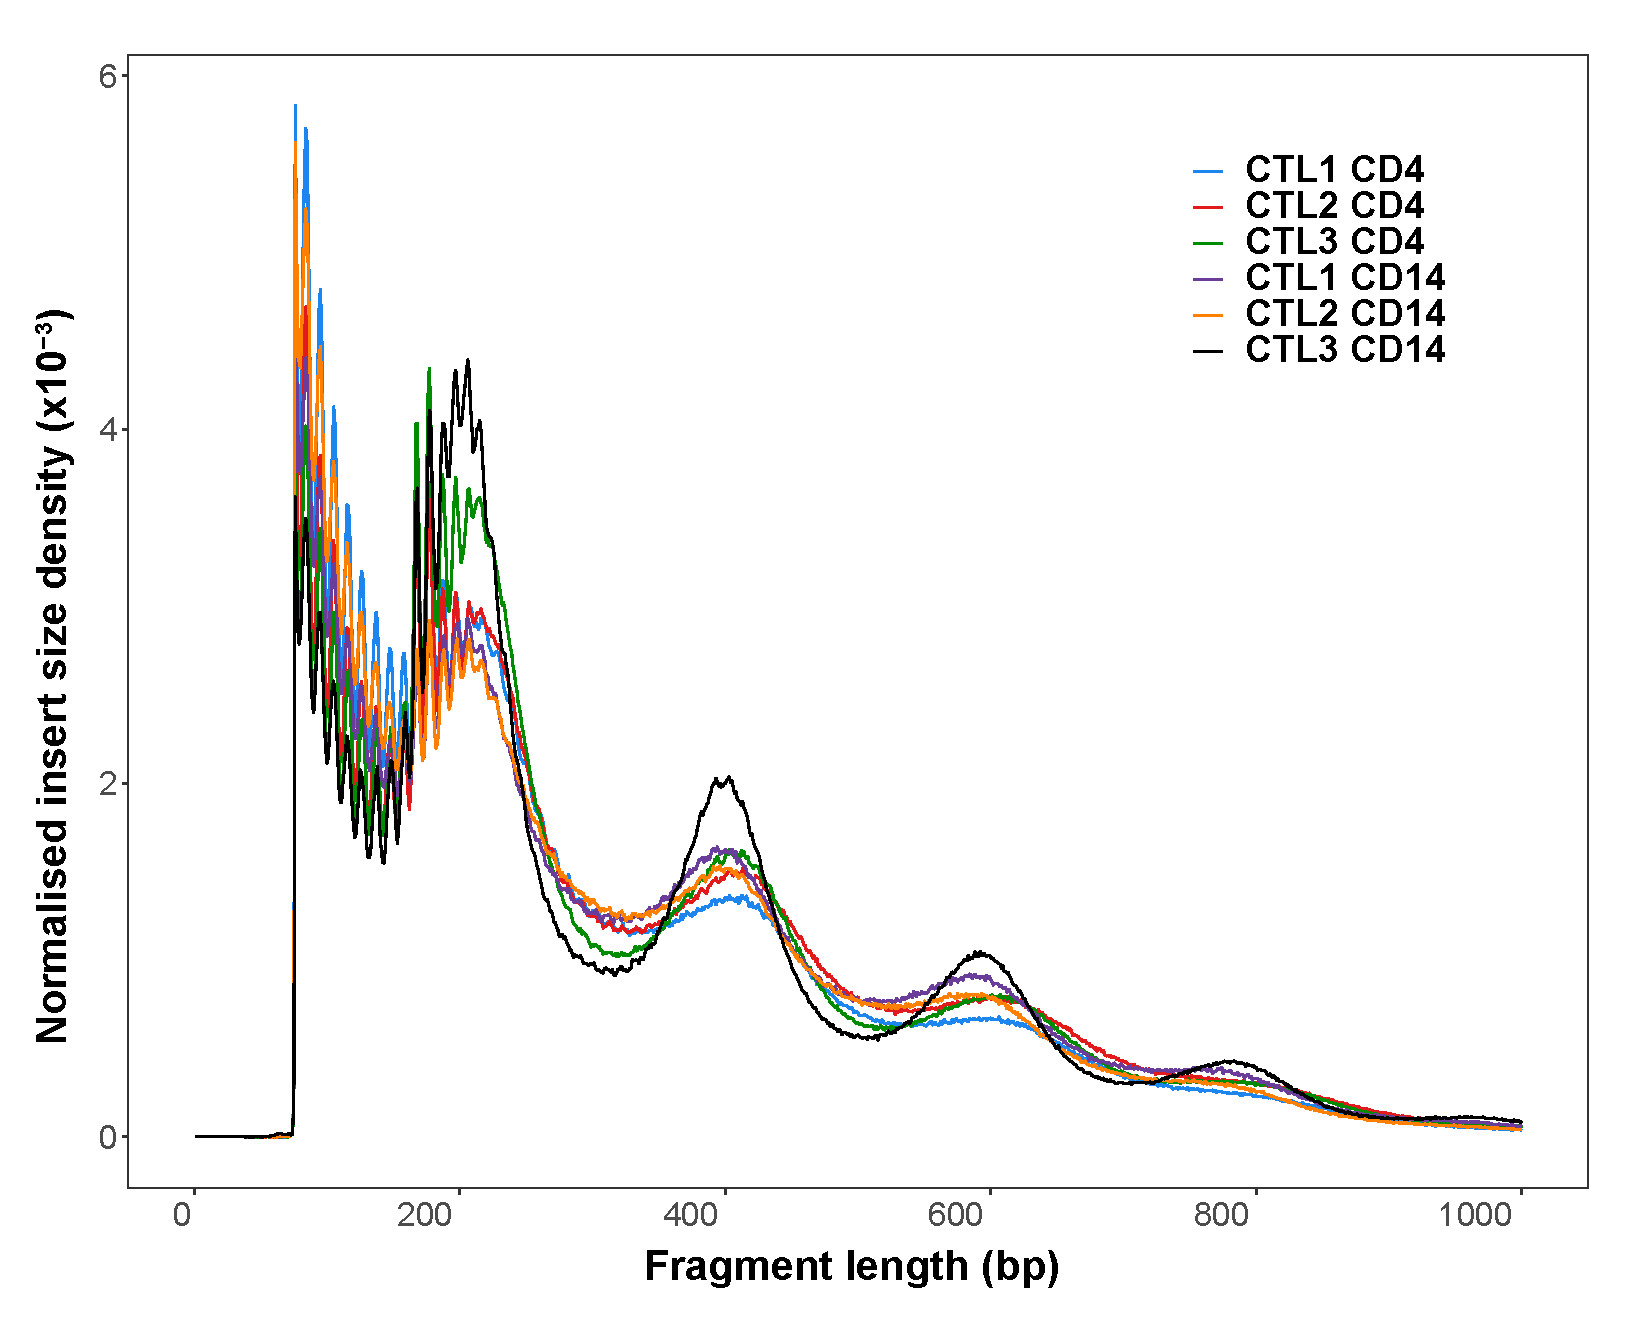
\includegraphics[width=\textwidth]{./Results1/pdfs/ATAC_Core_fresh_CD4_CD14_frag_size_distribution}
\caption{\textbf{}}
\end{subfigure}%
\begin{subfigure}[b]{0.45\textwidth}
\centering
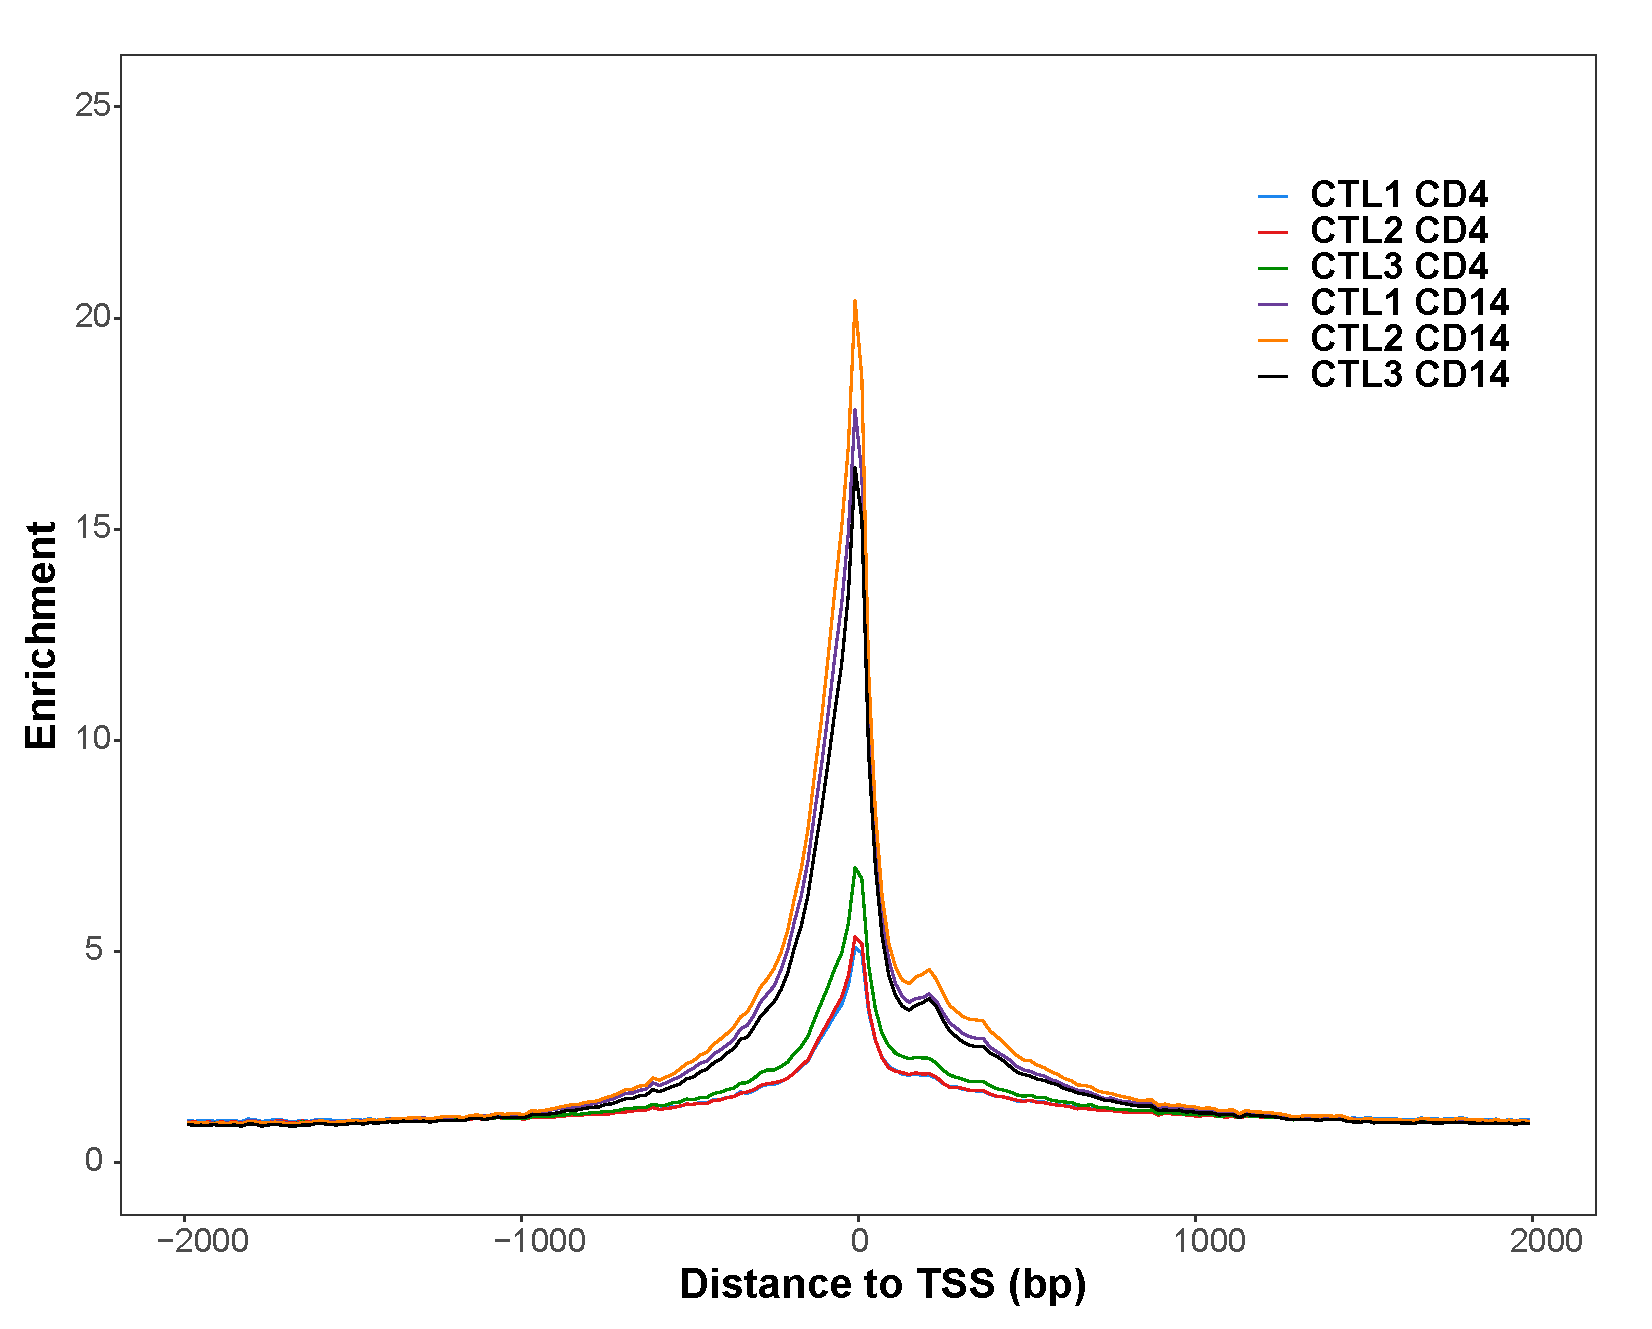
\includegraphics[width=\textwidth]{./Results1/pdfs/TSS_enrichment_Core_fresh_CD4_CD14}
\caption{\textbf{}}
\end{subfigure}
\begin{subfigure}[b]{0.6\textwidth}
\centering
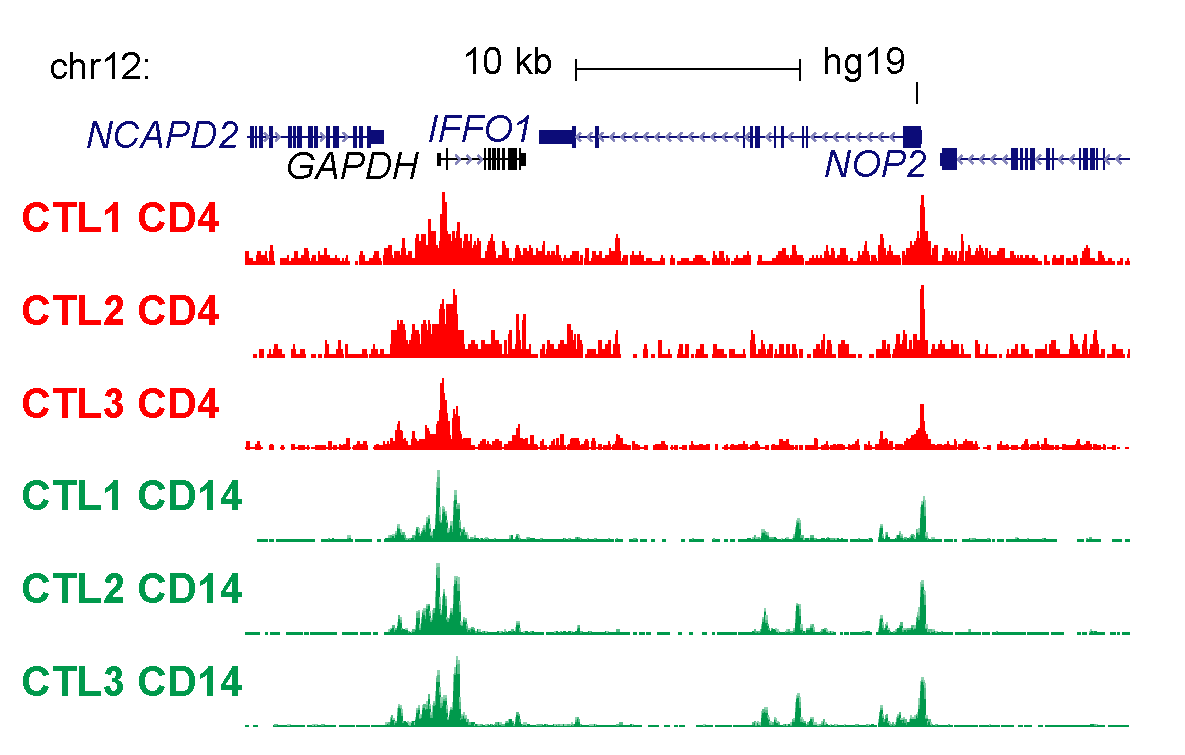
\includegraphics[width=\textwidth]{./Results1/pdfs/ATAC_Core_CD4_CD14_fresh_GAPDH}
\caption{\textbf{}} % to add text to the figure name
\end{subfigure}
\caption[Measurements for quality control assessment in ATAC-seq samples]{\textbf{Measurements for quality control assessment in ATAC-seq samples.} For each of the CD14$^+$ monocytes and CD4$^+$ samples used to establish the ATAC analysis pipeline quality control measures shown are (A) density distribution of ATAC-seq fragment sizes, (B) enrichment of ATAC-seq fragments across the TSS of all Ensembl genes and (C) UCSC Genome Browser view illustrating the ATAC-seq normalised read density (y-axis) at the promoters of \textit{GAPDH} and \textit{NOP2} genes. CD14$^+$ monocytes and CD4$^+$ tracks are colour-coded in green and red, respectively.}
\label{figure:QC_ATAC}
\end{figure} 

Another quality control measurement that was investigated and implemented was the enrichment of ATAC-seq signal over a random background of reads across all the TSS identified for Ensembl genes (Figure \ref{figure:QC_ATAC}B). This is a useful measure as nucleosome repositioning and an increase in chromatin accessibility occur at the TSS to allow TF binding and initiation of gene transcription. Fold-enrichment signals over the TSS ranged from 5 to 7 for the CD4$^+$ samples, and were much higher (17 to 20) in the CD14$^+$ samples. The lower sample quality of the CD4$^+$ compared to CD14$^+$ samples indicated by the TSS enrichment values were further evidenced by visualising the ATAC-seq read pile up at the promoters of the glyceraldehyde-3-phosphate dehydrogenase (\textit{GAPDH}) and the NOP2 Nucleolar Protein (\textit{NOP2}) gene, showing more background reads and lower signal for the tCD4$^+$ samples in red (Figure \ref{figure:QC_ATAC}C).
	
As part of the quality control assessment, the percentage of mitochondrial reads and the fraction of reads in peaks (FRiP) were also investigated (Table \ref{tab:ATAC_MT_fraction_reads_in_peaks}). 

\begin{table}[htbp]
%\setlength{\tabcolsep}{20pt} only to stretch the columns if you want
%\renewcommand{\arraystretch}{1.5}
\centering
\begin{tabular}{@{} c c c}
\toprule
\textbf{Sample} & \textbf{\% mitochondrial reads} & \textbf{Fraction of reads in peaks} \\
\midrule
\midrule
CTL1 CD4 & 14.9 & 9.8 \\
CTL2 CD4 & 30.5 & 11.2 \\
CTL3 CD4 & 28.8 & 11.6 \\
CTL1 CD14 & 43.3 & 32.2 \\
CTL2 CD14 & 36.8 & 57.0 \\
CTL3 CD14 & 37.6 & 49.9 \\
\bottomrule
\end{tabular}
\medskip %gap
\caption[ATAC-seq percentage of mitochondrial reads and fraction of reads in called peaks (FRiP).]{\textbf{ATAC-seq percentage of mitochondrial reads and fraction of reads in called peaks (FRiP).} The percentage of mitochondrial reads was calculated over the total number of sequencing reads (before filtering). FRiP was calculated as the proportion of ATAC-seq fragments overlapping significant peaks with standard filtering for all the samples (FDR$<$0.01).}
\label{tab:ATAC_MT_fraction_reads_in_peaks}
\end{table}
\bigskip %bigger space


FRiP score is an alternative to TSS enrichment for assessing the background signal in different types of assays that are based on peak calling, including ChIP-seq. Positive correlation between the TSS fold-change enrichment and FRiP was observed (data not shown), suggesting both are appropriate inter-dependent quality control measures to evaluate sample noise. For the 6 samples analysed here, mitochondrial content varied between (14.9-43.3\%), was higher in CD14$^+$ than in CD4$^+$ cells and was not directly related to any of the other quality control measurements. Therefore, mitochondrial reads in this range did not appear to reflect the samples quality and the main issue related to the need for deeper sequencing to achieve the desired number of non-mitochondrial reads for downstream analysis.

Both TSS and FRiP are appropriate signal-to-noise measures, with recommended threshold values from ENCODE and Alsoo and colleagues (Alasoo \texit{et al.}, 2018 and previously published in bioRxiv in 2017), being of FRiP between 10-20\% and TSS between 6-10. Importantly ENCODE has prioritised the use of TSS over FRiP as a more stable measure to determine the noise in the sample and therefore this was the chosen measure for this thesis. In summary from this analysis, all 6 samples showed appropriate ATAC-seq patterns of fragment size distribution, FRiP and TSS, with exception of CD4$^+$ CTL1 and CTL2, being borderline for the 6 fold-enrichment TSS threshold. 
%Importantly, this differences in the enrichment around the TSS successfully recapitulated the differences observed in the ATAC-seq density signal of the UCSC Genome Browser tracks between the CD14$^+$ and CD4$^+$ samples. These differences in ATAC-seq quality observed in these samples reflected the variability in performance of ATAC-seq and were useful in determining the influence of borderline sample quality in downstream analysis in order to choose the most robust strategy maximising the use of precious clinical samples. 
	

\subsubsection{Peak calling and filtering}
\label{peak_filtering}
Next, criteria for peak calling and filtering were investigated. Although different peak callers have been used to analyse ATAC-seq data, MACS2 has been methodology preferred by ENCODE and most publications (Table \ref{tab:ATAC_comparative_methods}). MACS2 was initially developed for ChIP data, but it has also been used for DHS and ATAC-seq disabling the model option and manually setting the shift (--shift) and extension size (--extsize) parameters, which refer to the number of bp and direction for the reads to be shifted and the number of bp for them to be extended, respectively. Since the --extsize should correspond to the average fragment size, this was set to 200bp which was the average fragment size calculated for the ATAC-seq libraries in this project. The --shift was set to -100, as it is recommended to be -1/2 of the fragment size when analysing chromatin accessibility data, such as DHS or ATAC-seq. 

A systematic analysis of the effect of sequencing depth and the sample quality on peak calling was conducted to better understand the effect of both variables on the downstream analysis. For each of the 6 samples, random sub-sampling of reads was performed in every 5 million increment, ranging from 5 to 30 total million reads, followed by peak calling with arbitrary filtering for false discovery rate (FDR)$<$0.01. The number of called peaks passing filtering showed a steady increase with read depth  (Figure \ref{fig:Peak_calling_versus_depth_ATAC}A), beginning to \textit{plateau} at approximately 25 million reads (Figure \ref{figure:Peak_calling_versus_depth_ATAC}B). Moreover, lower number of peaks were detected in CD4$^+$ samples compared to CD14$^+$ monocytes when using standard  FDR$<$0.01 filtering, highlighting the influence of sample quality on the total number of significant called peaks. Interestingly, sample quality as measured by FRiP (which relies on peak calling) showed very discrete changes with read depth and was stable from 15 million reads onwards for all six samples (Figure \ref{figure:Peak_calling_versus_depth_ATAC}C), similarly to TSS (data not shown). Overall, this confirmed that measurement of sample quality using FRiP or TSS was not affected by the sequencing depth.


\begin{figure}[htbp]
\centering
\begin{subfigure}{0.50\textwidth}
\centering
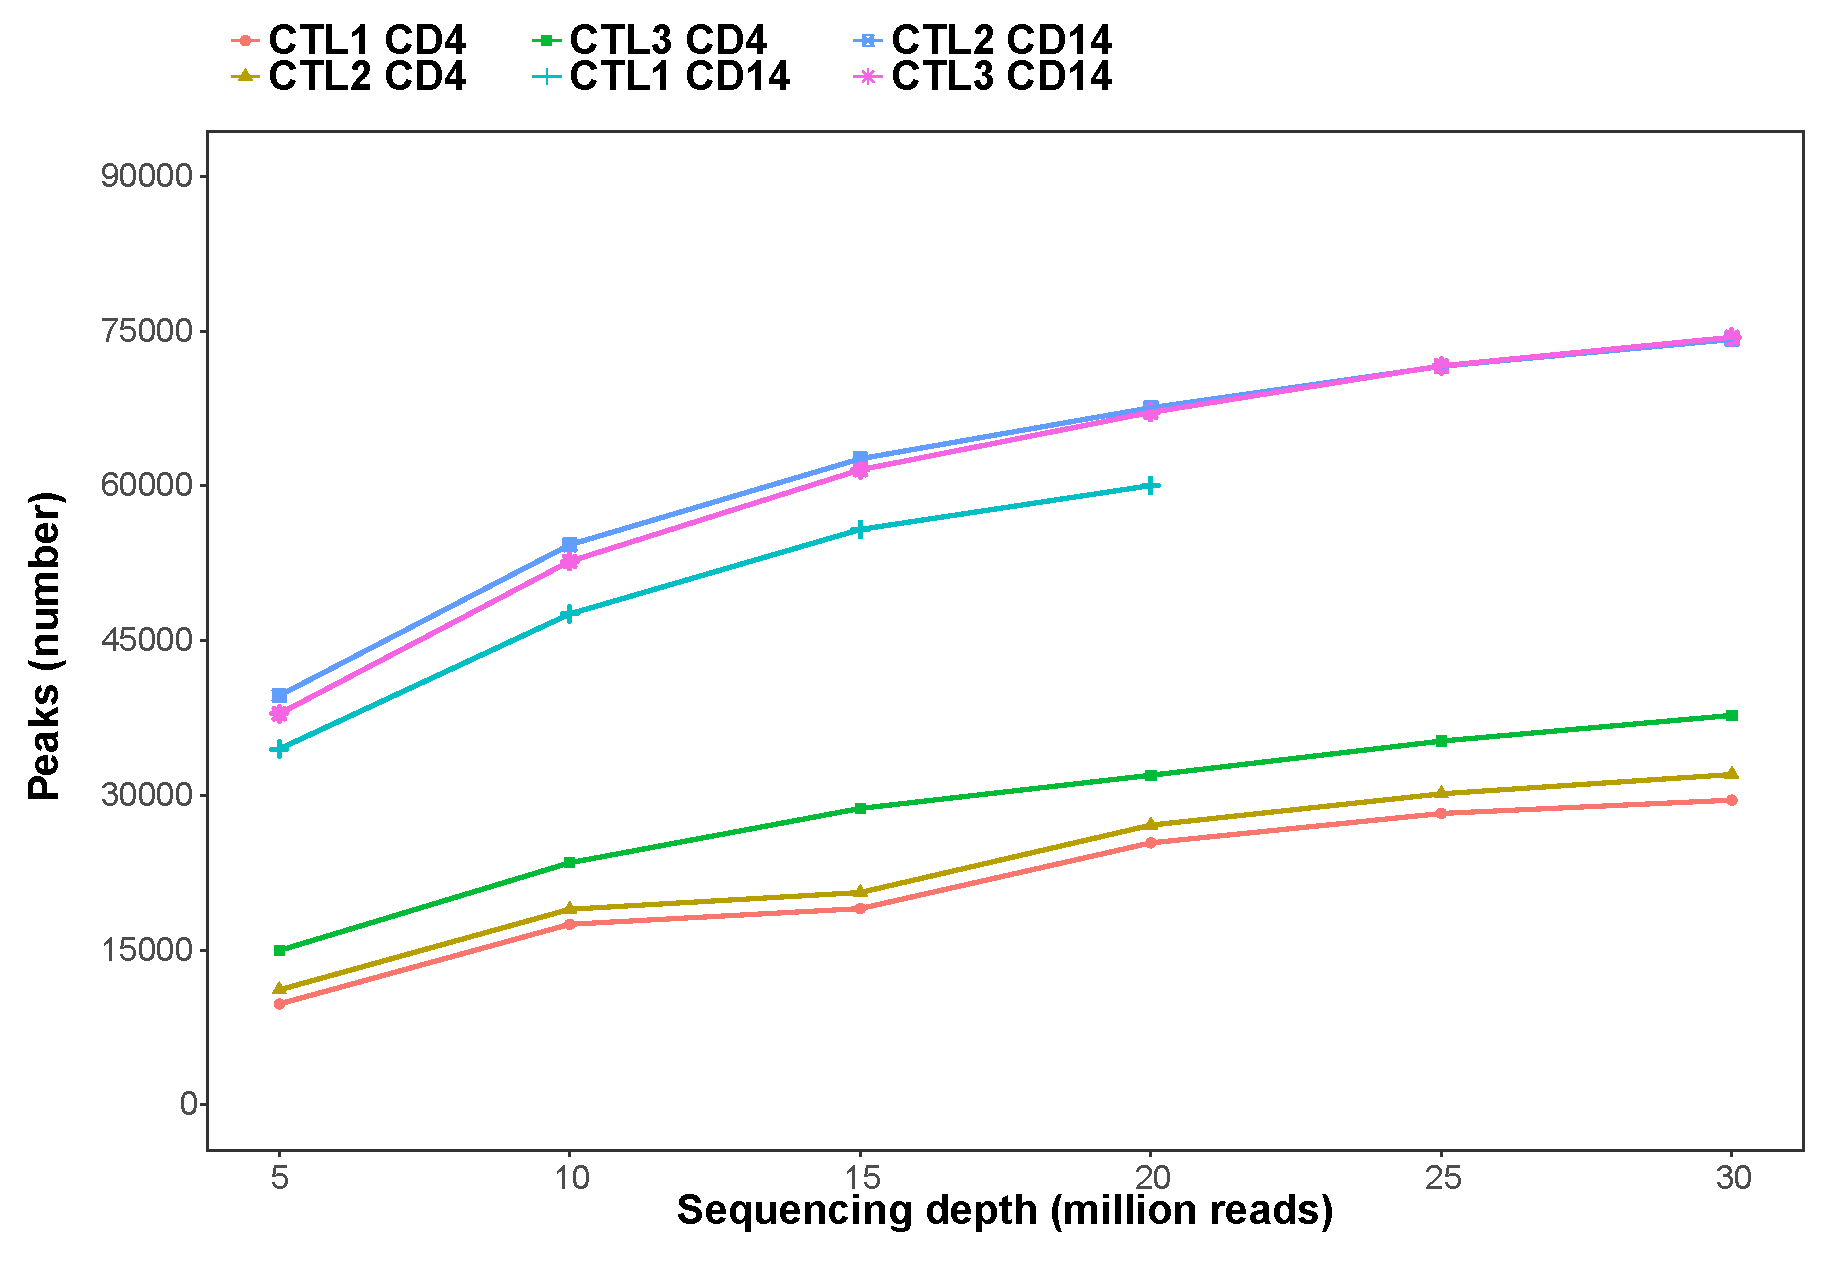
\includegraphics[width=\textwidth]{./Results1/pdfs/ATAC_Core_fresh_CD4_CD14_num_peaks_vs_depth}
\caption{\textbf{}}
% The percentage sign indicated that the other subfig goes side by side
\end{subfigure} \\
\begin{subfigure}{0.45\textwidth}
\centering
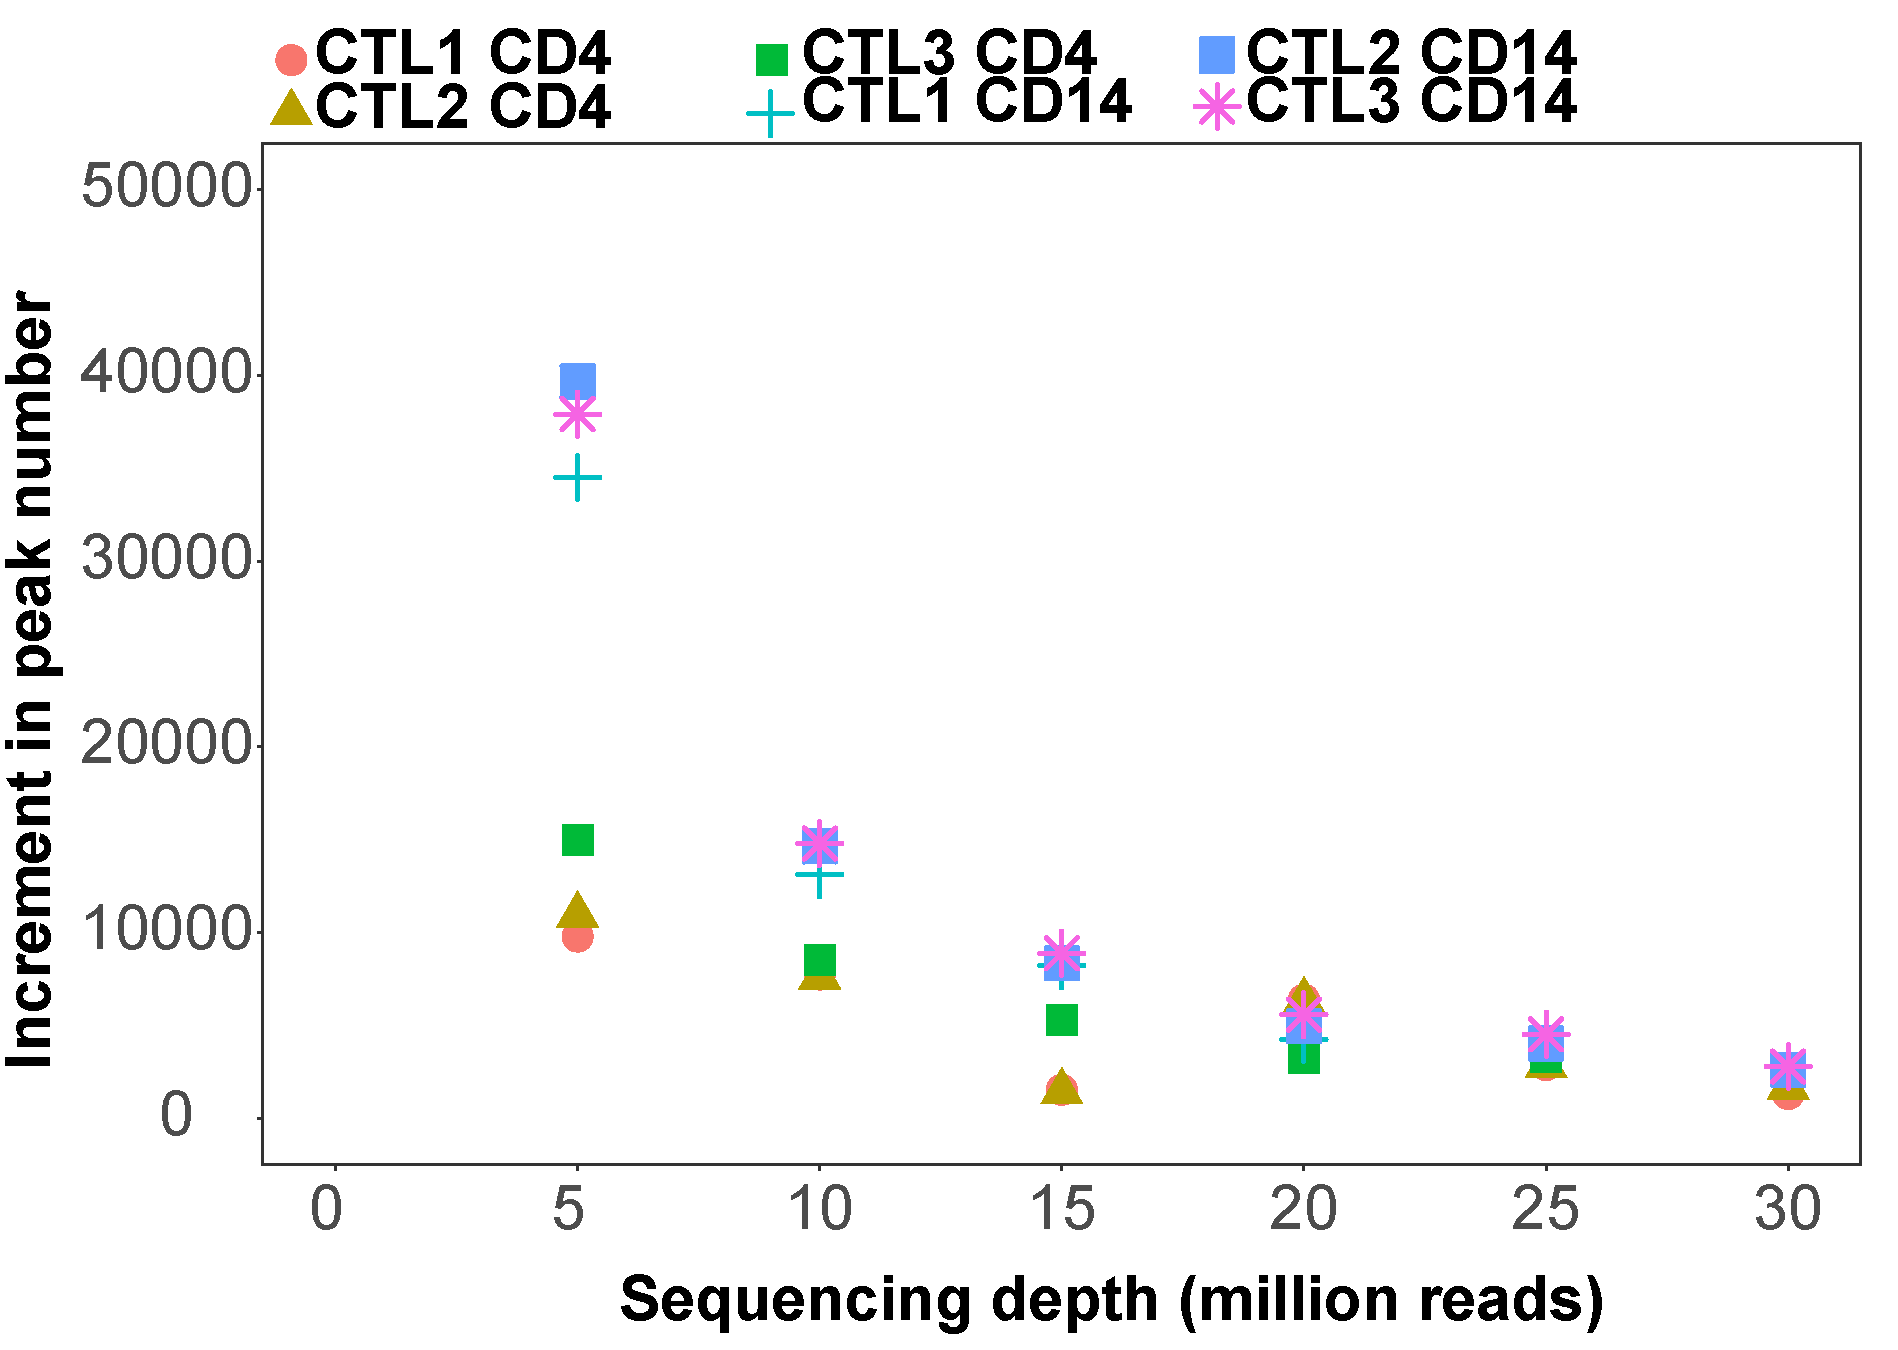
\includegraphics[width=\textwidth]{./Results1/pdfs/ATAC_Core_fresh_CD4_CD14_increment_num_peaks_vs_depth}
\caption{\textbf{}}
\end{subfigure} %
\begin{subfigure}{0.45\textwidth}
\centering
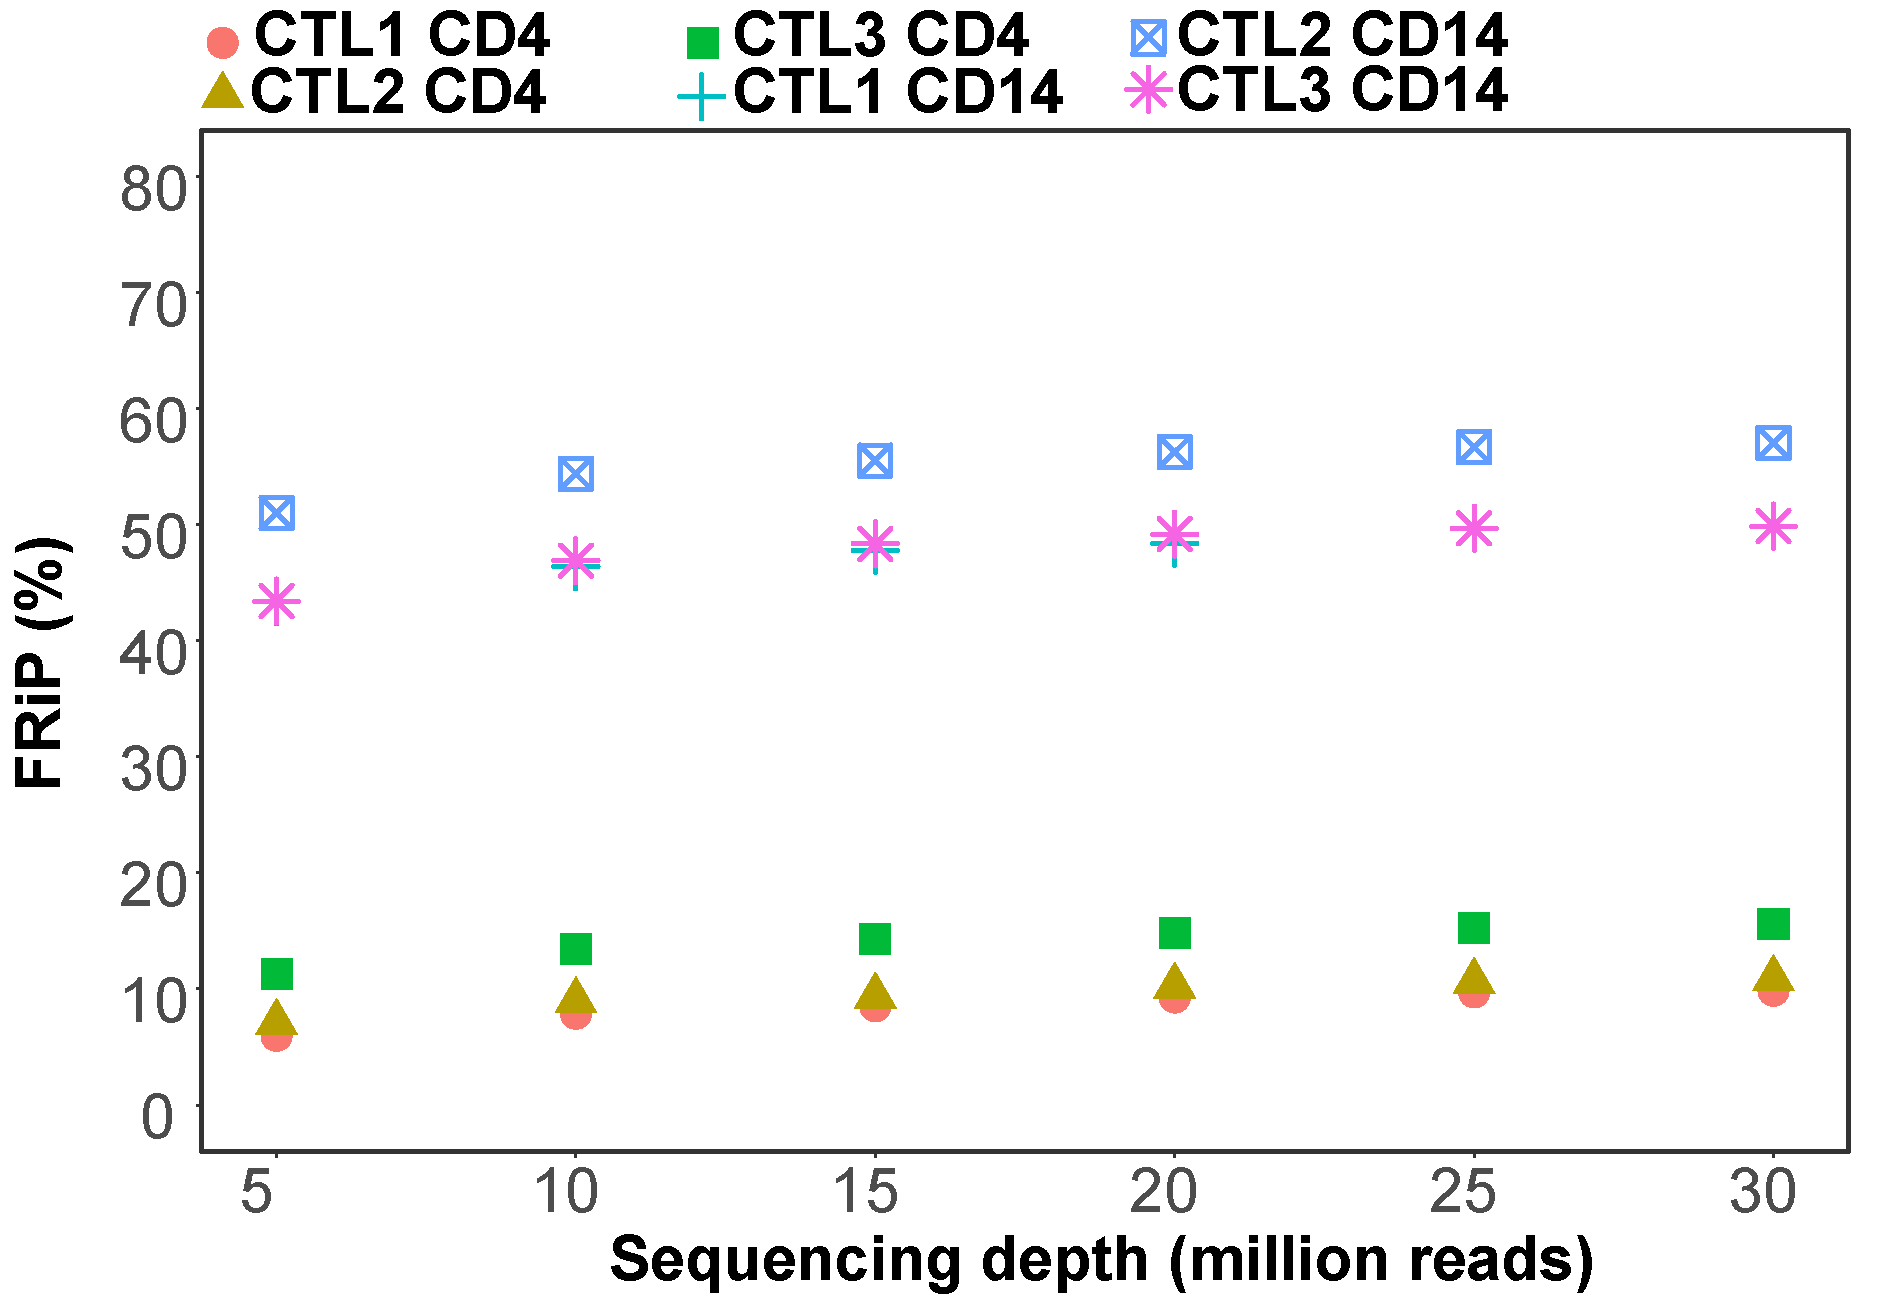
\includegraphics[width=\textwidth]{./Results1/pdfs/ATAC_Core_fresh_CD4_CD14_frac_reads_in_peaks_vs_depth}
\caption{\textbf{}}
\end{subfigure}
\caption[FRiP and peak calling at different sequencing depths in ATAC-seq libraries.]{\textbf{FRiP and peak calling at different sequencing depths in ATAC-seq libraries.} For a series of sequencing depths (from 5 to 30 million reads after filtering) representation of (A) number of called peaks (standard filtering using FDR$<$0.01, (B) the increment on the number of called peaks and (C) FRiP as a function of the sequencing coverage in the 6 samples included for the analysis in this section.}
\label{figure:Peak_calling_versus_depth_ATAC}
\end{figure} 



For peak filtering, an arbitrary FDR$<$0.01 in MACS2 is typically used (Table \ref{tab:ATAC_comparative_methods}) but may not remove low quality peaks equally successfully in lower quality samples and does not take into account the reproducibility of the called peaks. This IDR was used to experimentally identify the most appropriate p-value threshold to filter the called peaks in each individual sample. Filtered reads from each sample were partitioned in half to create two pseudoreplicates, peaks were called in each pseudoreplicate and the percentage of peaks sharing IDR rank position when filtered at decreasing pvals was calculated (Figure \ref{figure:Peak_calling_IDR_filtering_and_chrom_stated_ATAC}A and B). This strategy was tested across a range of total read counts (as above) to determine the effect of sequencing depth on the suitability of this peak calling filtering approach. The optimal pval giving the largest percentage of IDR shared peaks between the two pseudoreplicates varied more erratically when the sequencing depth was lower than 10 million reads (Figure \ref{figure:Peak_calling_IDR_filtering_and_chrom_stated_ATAC}A and B), suggesting this analysis was not appropriate for lower read depths. This variation was more pronounced and extended in CD4$^+$ T cells, which had lower TSS values compared to CD14$^+$ monocytes ATAC-seq libraries (representative examples of CTL2 CD4$^+$ and CD14$^+$ monocytes in Figure \ref{figure:Peak_calling_IDR_filtering_and_chrom_stated_ATAC}A and B). The shape of the curves were also influenced by the sample quality. For appropriate sequencing depth (15-20 million reads), the CD14$^+$ monocytes (TSS enrichment $\geq$10) samples presented a profile reaching a single maximum of shared IDR peaks for a particular filtering pval (Figure \ref{figure:Peak_calling_IDR_filtering_and_chrom_stated_ATAC}B), which was -log10 pval 8 in all three samples (data not shown). In contrast, the same analysis in CD4$^+$ samples revealed two pvals for which the percentage of IDR shared peaks reached two local maxima (Figure \ref{figure:Peak_calling_IDR_filtering_and_chrom_stated_ATAC}A). 



\begin{figure}[htbp]
\centering
\begin{subfigure}{0.45\textwidth}
\centering
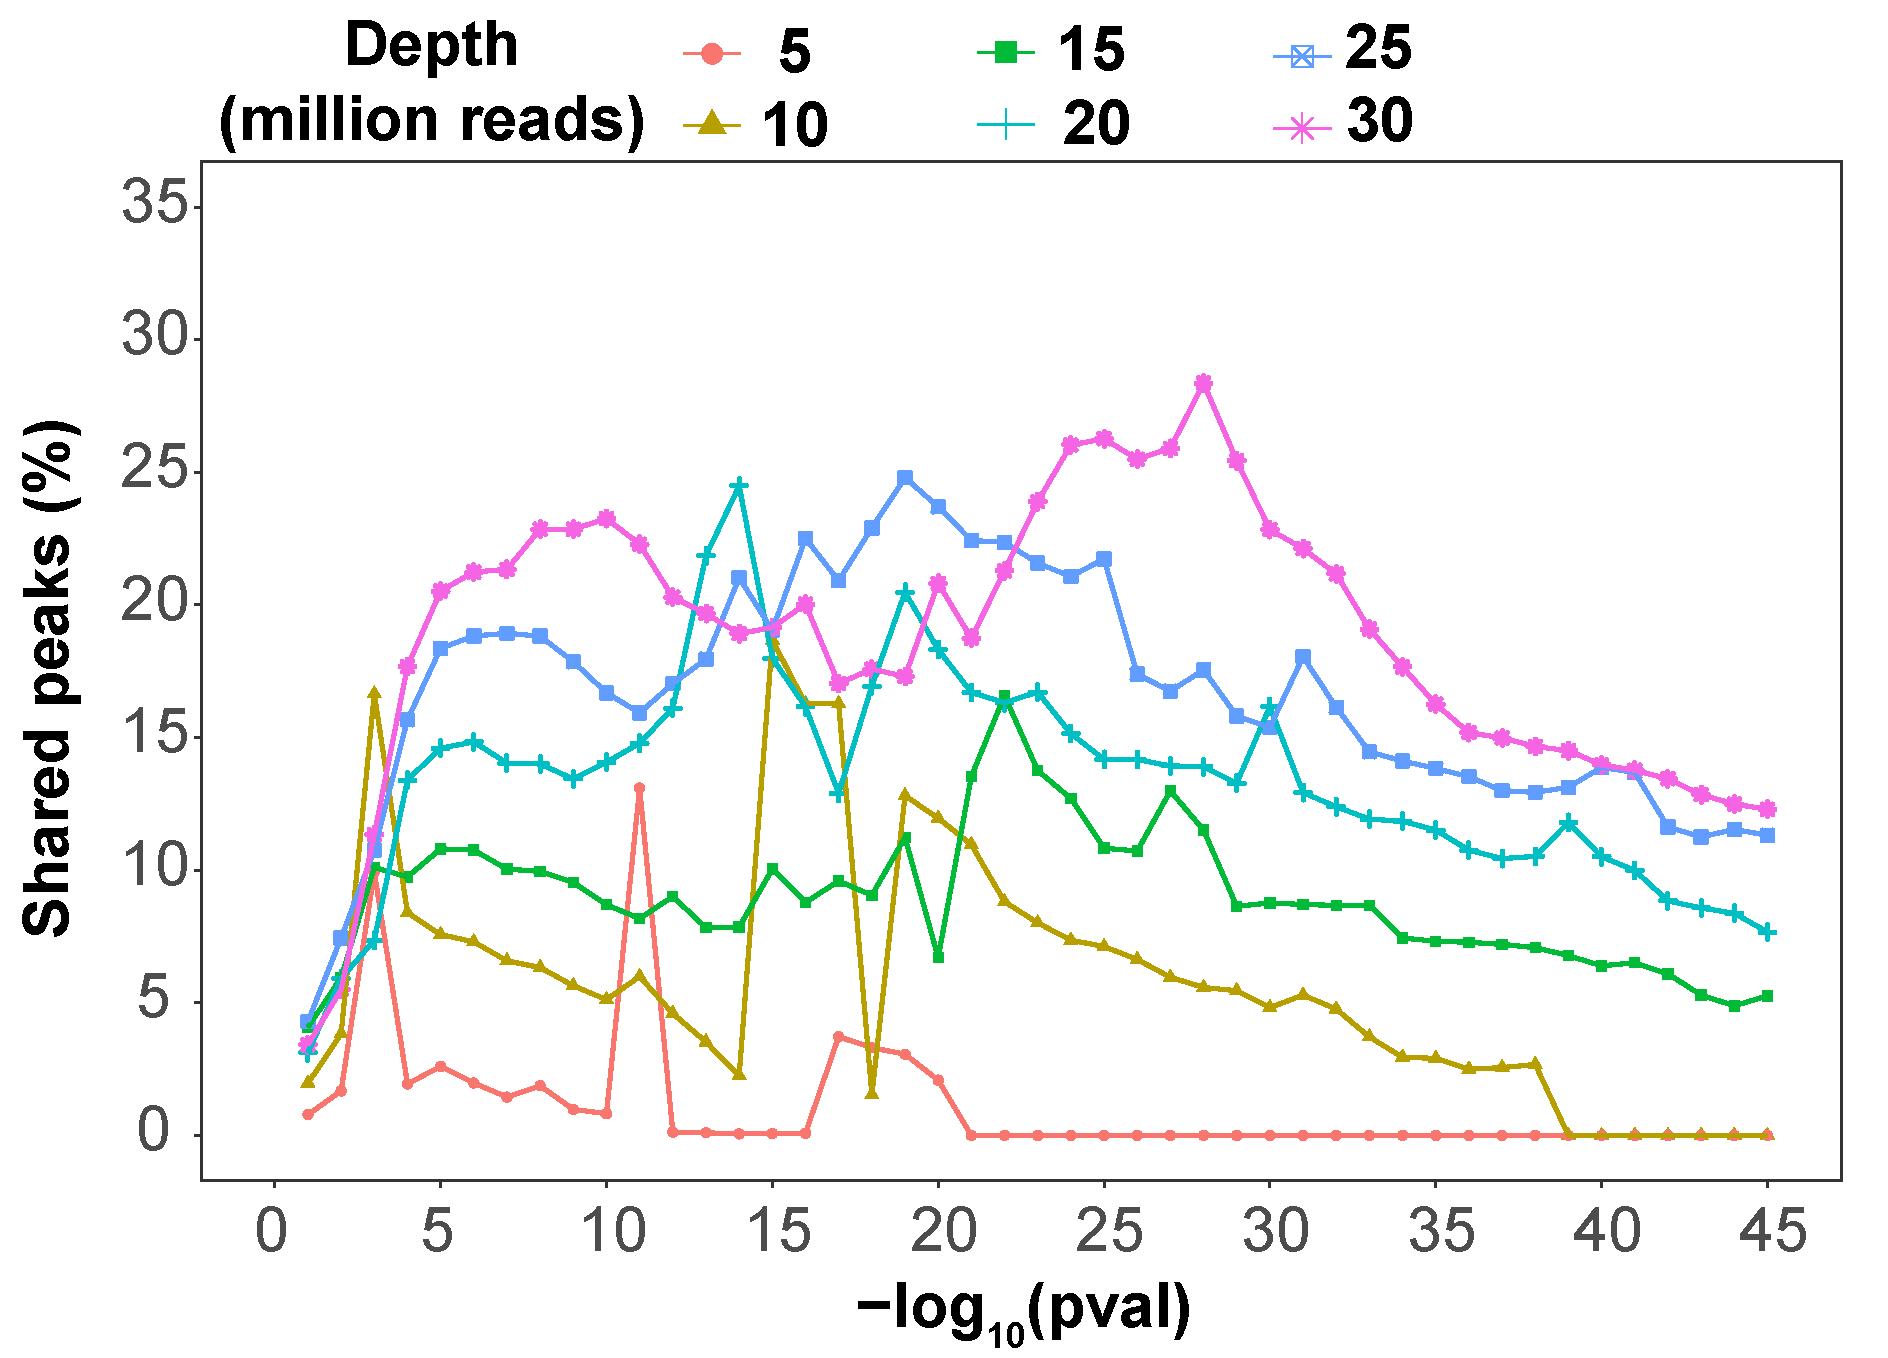
\includegraphics[width=\textwidth]{./Results1/pdfs/ATAC_Core_fresh_CTL2_CD4_shared_peaks_IDR_vs_pval}
\caption{\textbf{}}
% The percentage sign indicated that the other subfig goes side by side
\end{subfigure}%
\begin{subfigure}{0.45\textwidth}
\centering
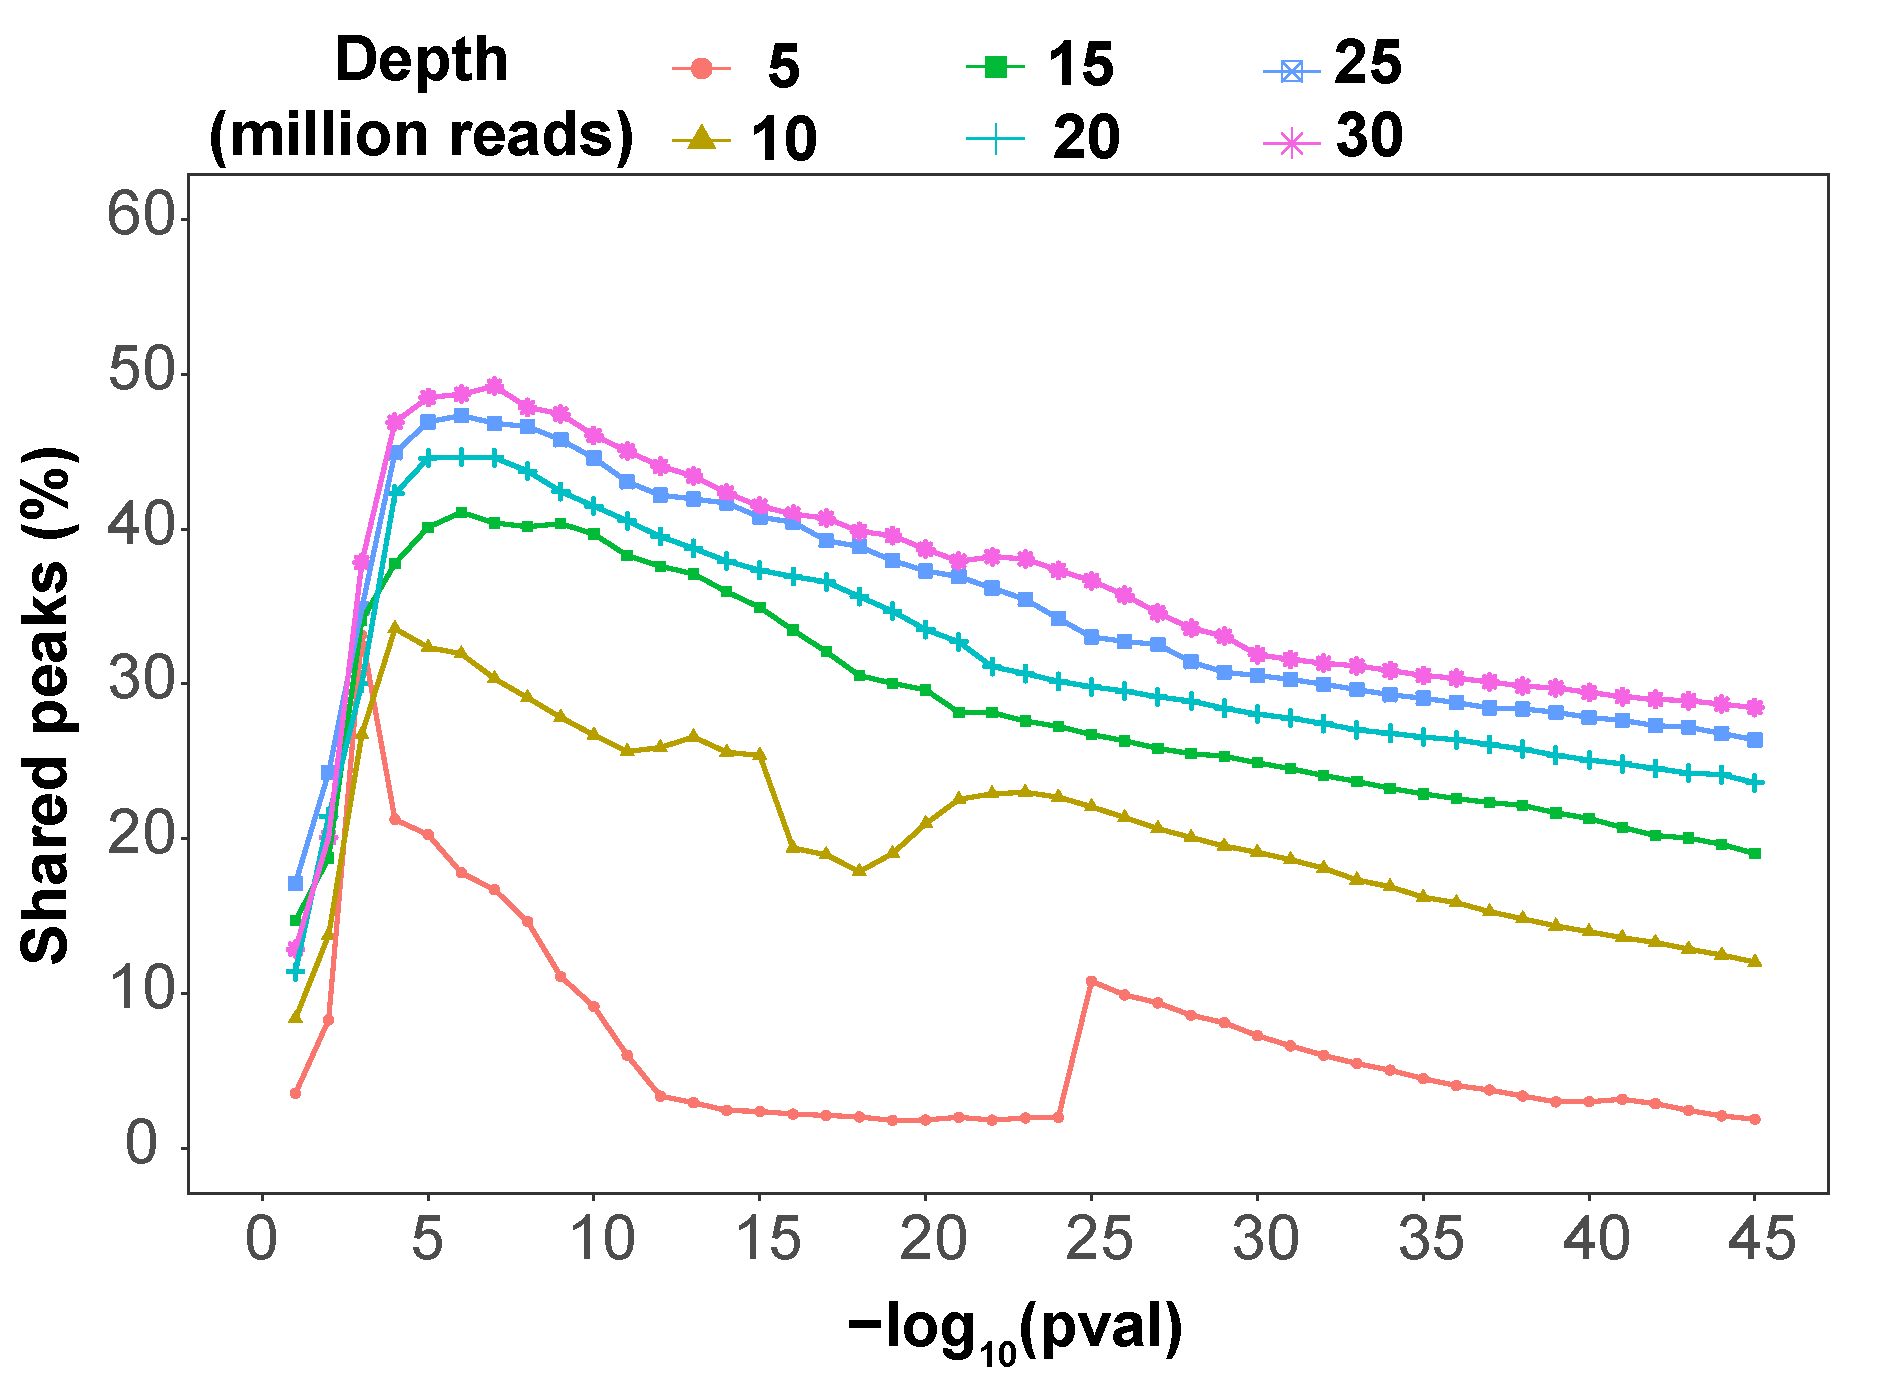
\includegraphics[width=\textwidth]{./Results1/pdfs/ATAC_Core_fresh_CTL2_CD14_shared_peaks_IDR_vs_pval}
\caption{\textbf{}}
\end{subfigure} \\
\begin{subfigure}{0.65\textwidth}
\centering
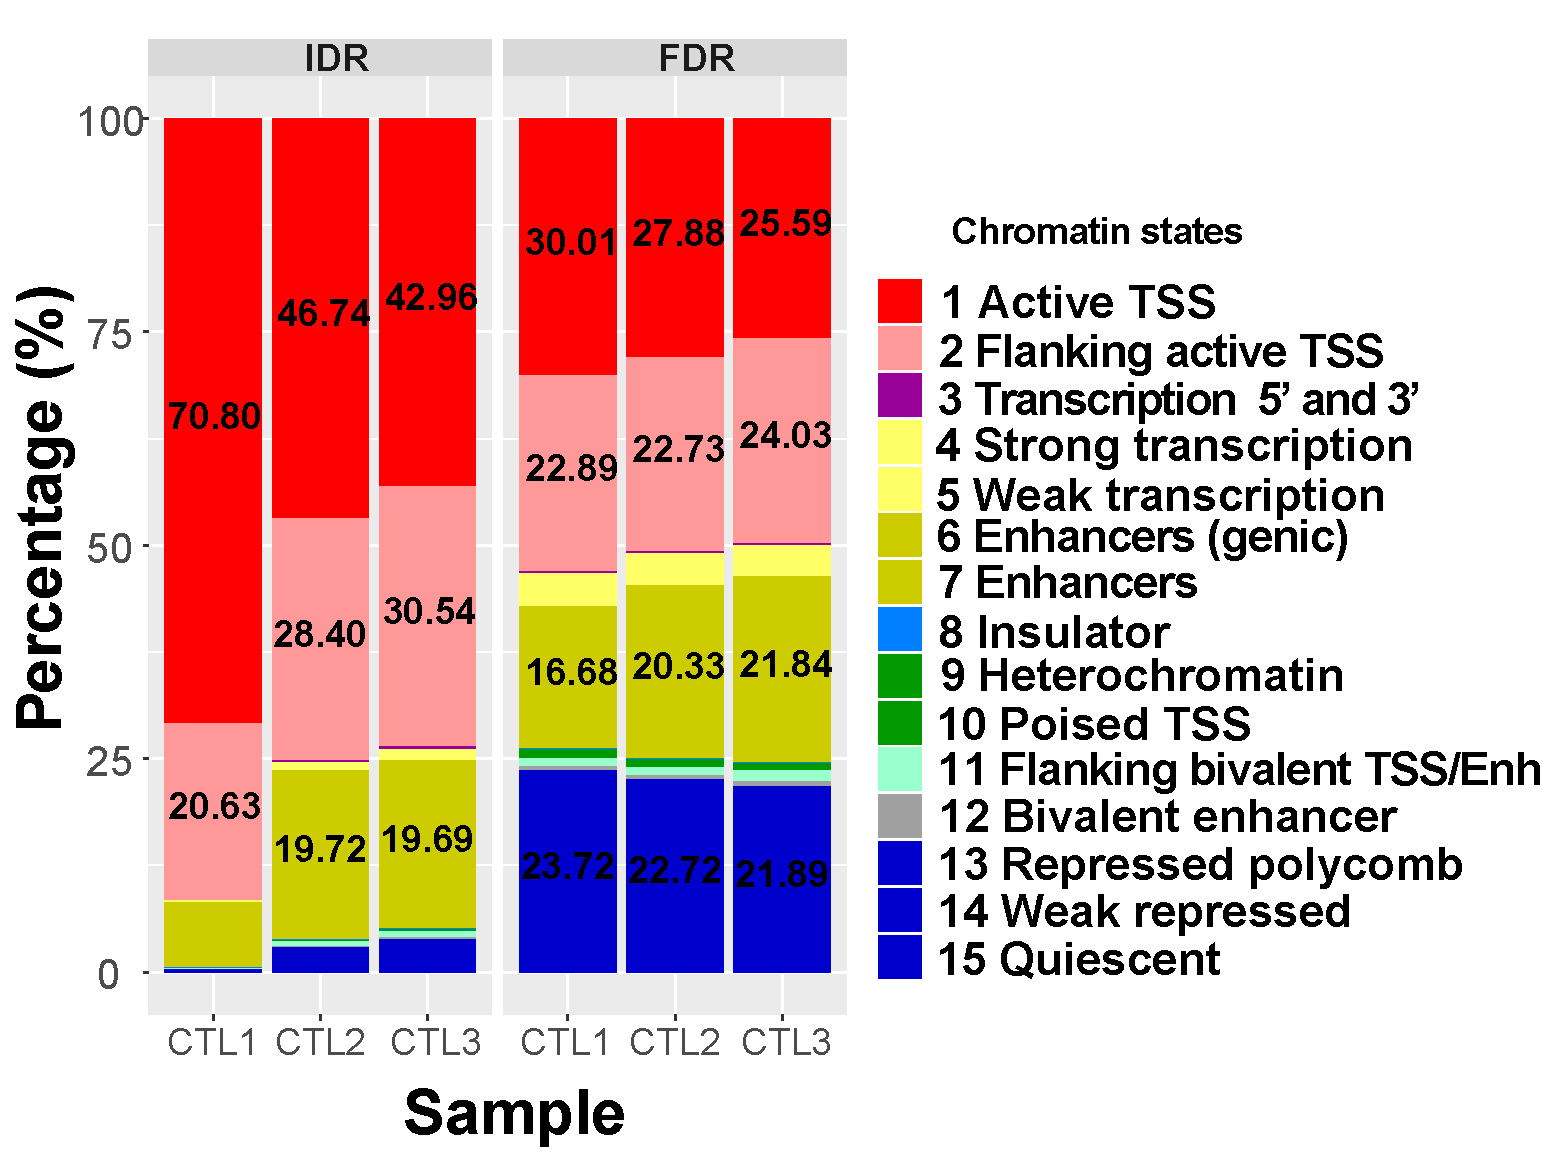
\includegraphics[width=\textwidth]{./Results1/pdfs/stacked_barplot_chromatin_states_percent_CD4_qval_vs_PVAL_IDR_filtered}
\caption{\textbf{}} % to add text to the figure name
\end{subfigure}%
\caption[Peak calling filtering using IDR analysis in ATAC-seq samples.]{\textbf{Peak calling filtering using IDR analysis in ATAC-seq samples.} For each of the sequencing depths tested (from 5 to 30 million reads after filtering), an illustration of the percentage of peaks sharing IDR rank between the two pseuroreplicates is shown when using different pval filtering thresholds in CTL2 (A) CD14$^+$ monocytes and (B) CD4$^+$ (used as representative samples differing in quality for this analysis). (C) Annotation (as percentage of total) of the CTL1, CTL2 and CTL3 CD4$^+$ ATAC-seq peaks filtered for FDR$<$0.01 or optimal pval from the IDR analysis (pval=10$^-11$) with the corresponding cell type specific Roadmap Epigenomics Project chromatin segmentation map.}
\label{figure:Peak_calling_IDR_filtering_and_chrom_stated_ATAC}
\end{figure} 


Filtering the CD4$^+$ peaks at the pval of the first local maximum (10$^{-11}$) reduced the percentage of peaks overlapping regions,  suggestive of noise (e.g heterochromatin, repetitive sequences and repressed regions) when compared to using the list of significant peaks filtered based on FDR$<$0.01 (Figure \ref{figure:Peak_calling_IDR_filtering_and_chrom_stated_ATAC} c). In summary, this IDR analysis provided a systematic method to identify an optimum pval with which to perform sample-specific filtering of technically reproducible peaks when the sequencing depth was over 10 million reads. These resulting filtered peaks will be used downstream to build the master list of regions across all the samples and perform differential chromatin accessibility analysis. 

%Should mention that the median of all this first max are used to perform filtering for all the samples because following other pipelines they always use same filtering value for all samples so we need to be consistent across samples


\subsubsection{Differential chromatin accessibility analysis}

In this thesis, a peak-based approach using the number of read counts overlapping the peaks included in the consensus master list (ML\_all) was implemented to perform differential analysis. One of the main limitations of the ATAC-seq and Fast-ATAC protocols (discussed in \ref{ATACseq} and \ref{Fast_ATAC}) is the background signal. Therefore, an empirical cut-off was identified to minimise the impact of background read counts on the peaks included for the differential analysis \parencite{Xinmin2005,Jonker2014}. Moreover, due to lack of consensus in terms of normalisation and differential analysis methods in ATAC-seq (as reviewed in Table \ref{tab:ATAC_comparative_methods}), two strategies were tested (Figure \ref{figure:ML_workflow}). \ToDo{The first one involved quantile normalisation of the reads mapping to each of the ATAC-seq accessible regions and the use of limma voom to perform differential chromatin accessibility analysis. The second strategy relied on the use of DESeq2 for both, normalisation and differential analysis.}


\begin{landscape}
\begin{figure}[htbp]
\centering
\includegraphics[width=1.2\textwidth]{./Results1/pdfs/ATAC_master_list_filtering_flow_chart}
\caption[Work flow illustrating the strategy to account for ATAC background noise prior to differential analysis.]{\textbf{Work flow illustrating the strategy to account for ATAC background noise prior to differential analysis.} A combined consensus peak master list (ML\_all) was built as explained in Chapter \ref{ch:Mat}, including all the significant peaks from each sample that were shared by at least 30\% of the total number of samples included in the analysis. The peaks were further transformed to obtain non-overlapping 500bp homogenous entities. The data regarding the ML\_all can be represented by two matrices (Step 1). The first one is the significance matrix with each entry indicating the significance of a peak (in rows) in each sample (in columns) as in presence (1, significant) or absence (0, non-significant). The second matrix is the count matrix storing the number of reads mapped to the peak (in rows) for each sample (in columns). A density distribution plot was generated with the read counts from the absent peaks (0) in each sample and used to define a sequence of twenty cut-offs illustrating the number of counts showed by a particular percentage of the total absent peaks (background counts) (Step 2). The defined cut-off were used to filter out peaks from the ML\_all and generate a series of reduced matrices (Step 3) that were tested for normalisation and differential chromatin accessibility analysis by two methods (quantile\&limma voom or DESeq2) (Step 4).}
\label{figure:ML_workflow}
\end{figure}
\end{landscape}



From the count matrix for the 6 samples defined above, the read counts from those peaks that were absent in each sample (since the  ML\_all includes peaks present in at least 30\% of the total samples)(Figure \ref{figure:ML_workflow} Step 1) were used to generate a density distribution plot (Figure \ref{figure:ML_workflow} Step 2). From this plot, a sequence of twenty cut-offs were defined, with each representing the number of counts showed by a particular percentage of the total absent peaks (Figure \ref{figure:ATAC_absent_peaks_distribution}). Each cut-off was used to filter out peaks from the ML\_all raw count matrix whose values in more than three samples were lower than the background counts (Figure \ref{figure:ATAC_absent_peaks_distribution} Step 3). A filter of three samples were chosen, as it corresponds to the smallest group of replicates in this particular experimental design and ensures peaks absent in one condition were retained. As a result, each cut-off generates a reduced matrix of low-noise peaks that was normalised using quantile or DESeq2 (library size and variance stabilisation \parencite{Love2014}) and used to conduct differential analysis with limma voom or DESeq2, respectively. Both normalisation methods performed appropriately for all the reduced master lists across the 6 samples, with slightly greater consistency for the quantile normalisation across the two groups (Figure \ref{figure:ATAC_normalisation_and_DARs_limma_DESeq2}A and B). Differential chromatin accessibility analysis using quantile normalisation counts\& limma voom showed a greater number of significant (FDR$<$0.01 and fold change$>$1.5) differentially accessible regions (DARs) compared to DESeq2, across all filtering cut-offs (Figure \ref{figure:DOC_quantile_DESeq2}C). The two approaches presented a progressive decrease in the number of DARs from the 75\% cut-off onward, suggesting a reduction in the number of false positive hits reported for peaks with read counts close to the background noise cut-off. Further increases in the cut-off value however are expected to also remove true positives, so an intermediate value is chosen here. Depending on the noise inherent to an experiment this threshold may vary. 

\begin{figure}[htbp]
\centering
\begin{subfigure}{0.45\textwidth}
\centering
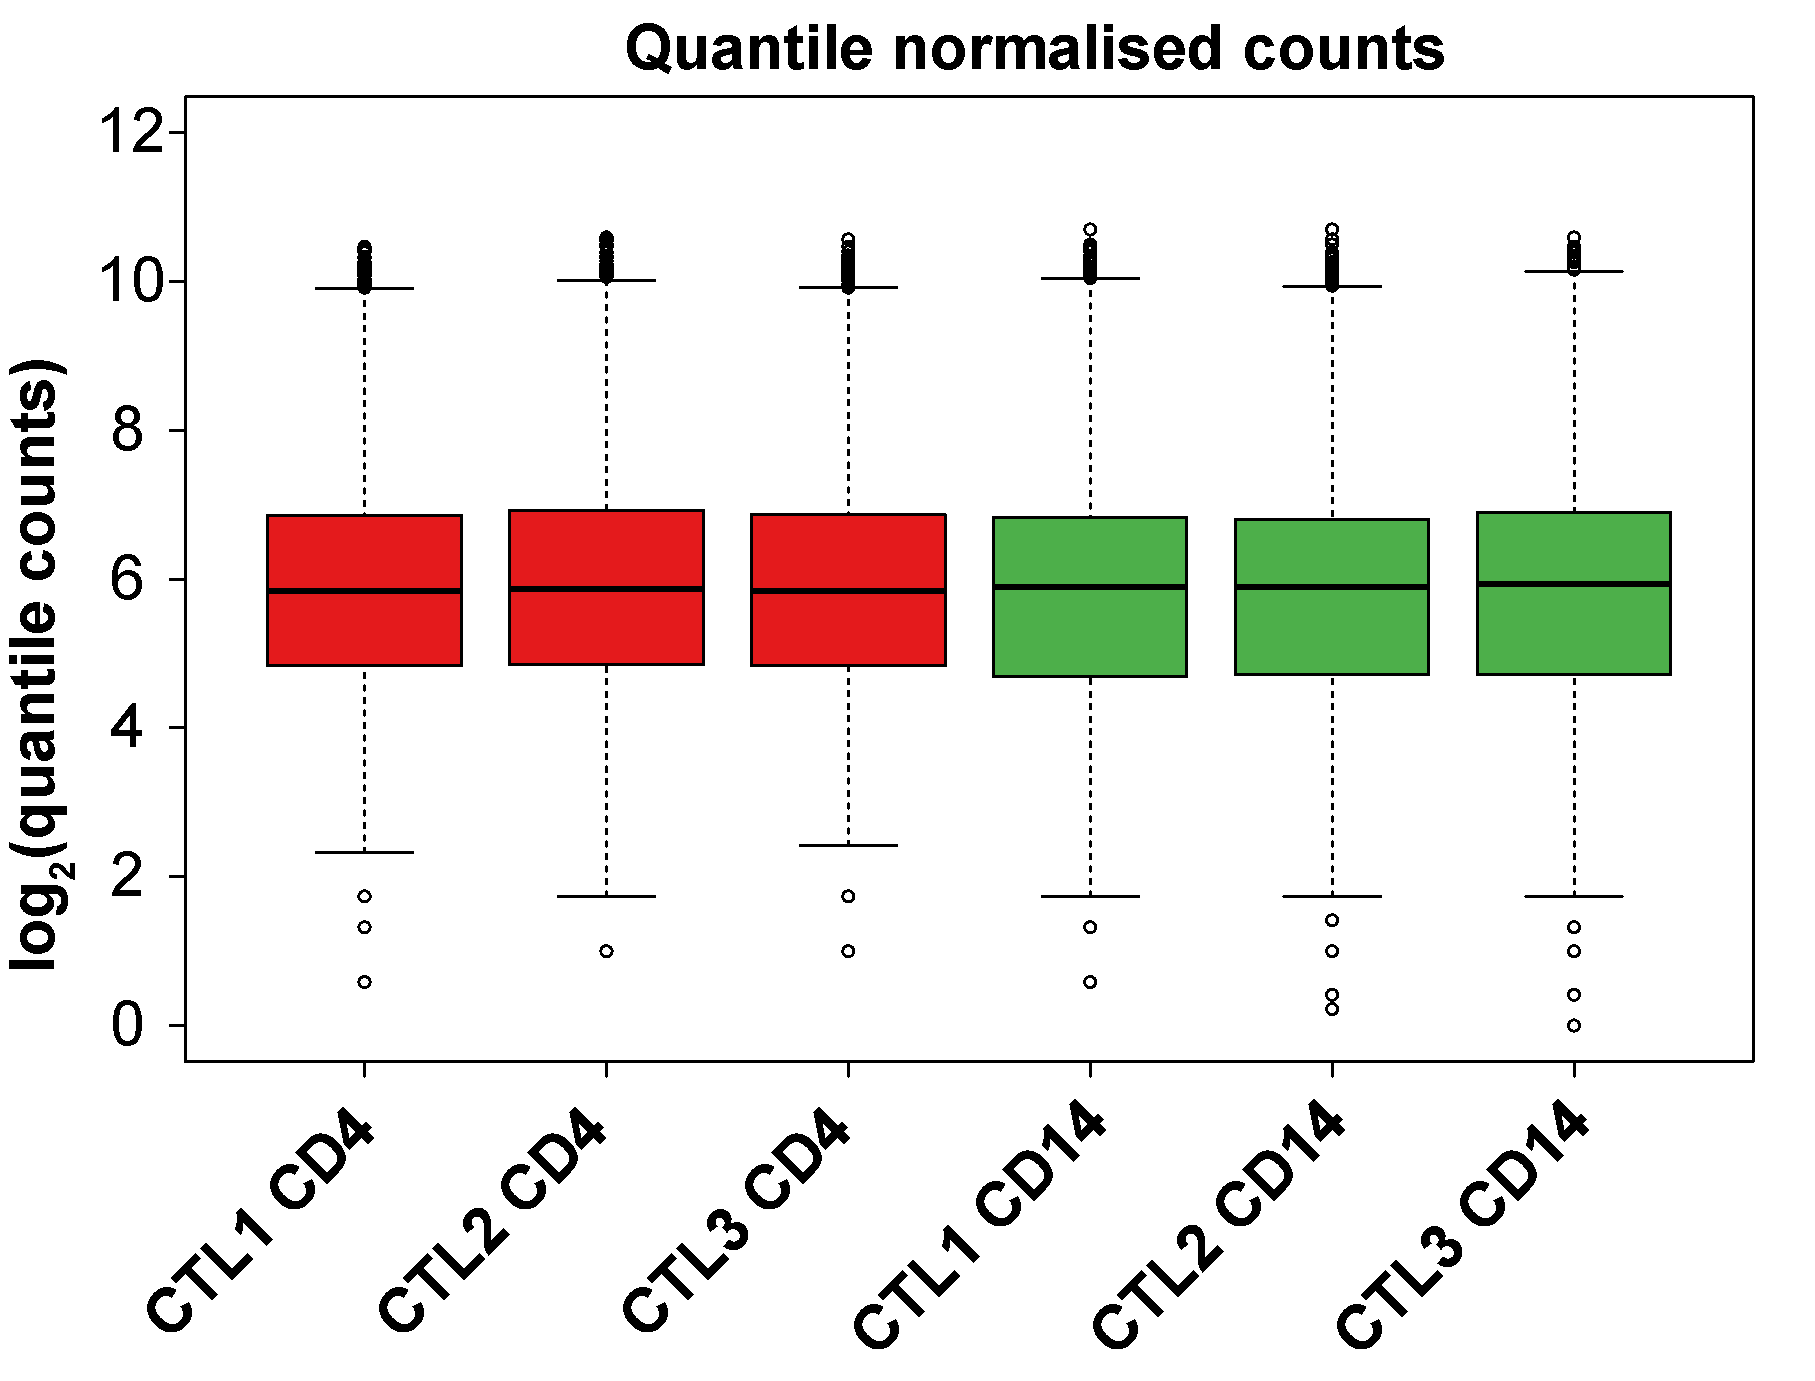
\includegraphics[width=\textwidth]{./Results1/pdfs/ATAC_Core_CD4_CD14_boxplot_80pcnt_cut_off_filtered_quantile_counts}
\caption{\textbf{}}
\end{subfigure}%
\begin{subfigure}{0.45\textwidth}
\centering
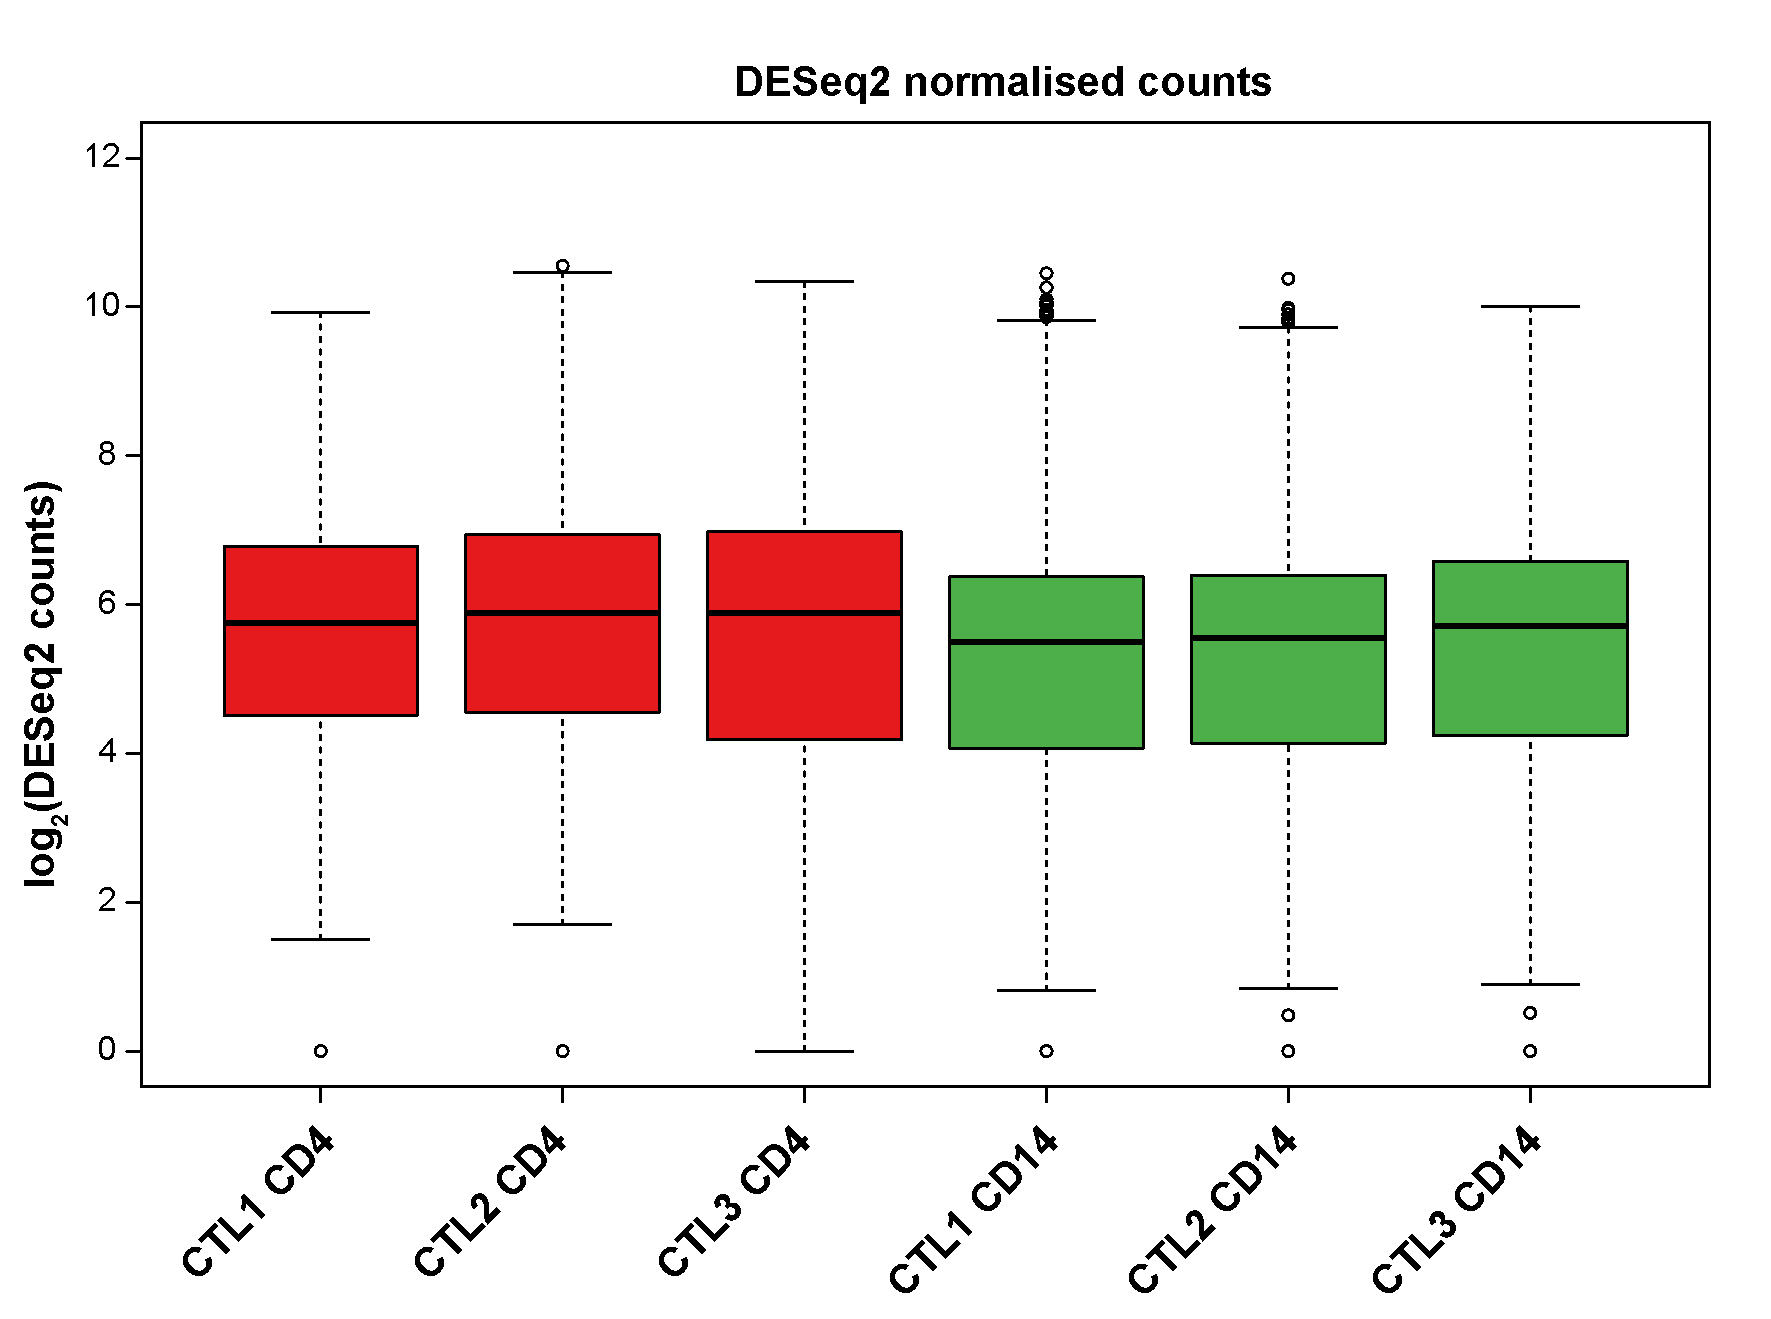
\includegraphics[width=\textwidth]{./Results1/pdfs/ATAC_Core_fastq_CD4_CD14_DESeq2_mean_vs_log2sd}
\caption{\textbf{}}
\end{subfigure}
\begin{subfigure}{0.5\textwidth}
\centering
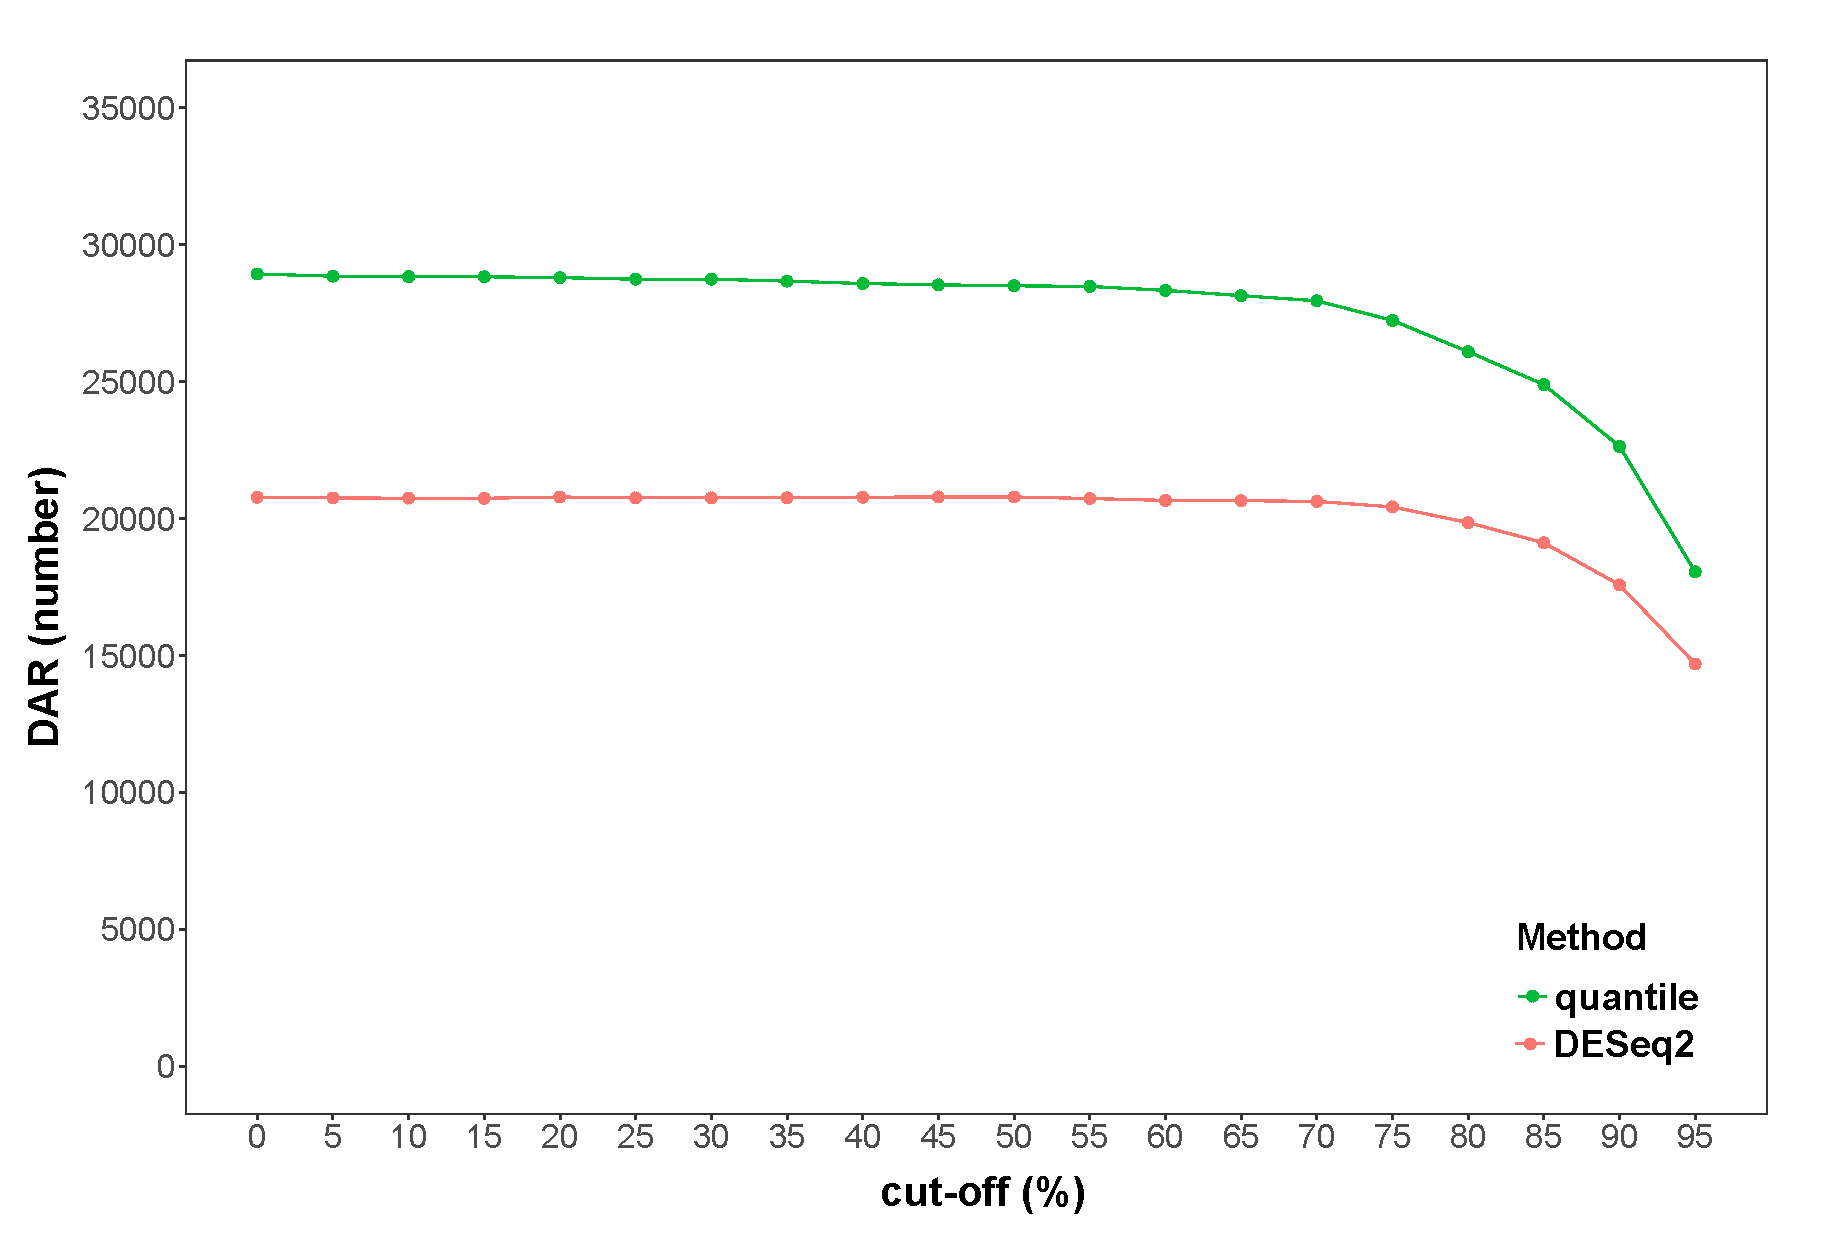
\includegraphics[width=\textwidth]{./Results1/pdfs/ATAC_Core_CD4vsCD14_DOC_FDR_01_vs_cutoffs_quantile_DESeq2_only}
\caption{\textbf{}}
\end{subfigure}

\caption[Normalisation and differential chromatin accessibility analysis for different cut-offs using quantile normalisation limma voom and DESeq2.]{\textbf{Normalisation and differential chromatin accessibility analysis for different cut-offs using quantile normalisation\&limma voom and DESeq2.} Boxplots representing the log$_2$  read counts for each of the peaks from the unfiltered master list normalised by (A) quantile or (B) DESeq2 in the three CD14$^+$ monocytes and total CD4$^+$  healthy control paired samples. (C) Representation of the number of significant DARs (FDR$<$0.01 and FC$>$1.5) detected in the differential analysis by limma voom (using quantile normalisation) or DESeq2 when using a sequence of empirical background noise cut-offs to filter the peak master list.}
\label{figure:ATAC_normalisation_and_DARs_limma_DESeq2}
\end{figure} 


From this analysis, 80\% was chosen as a conservative filtering cut-off, with the vast majority of the 19,855  DARs called as significant using the more conservative method (DESeq2) recapitulated by limma voom at the same significance threshold (FDR$<$0.01 and fold change$>$1.5) (Figure \ref{figure:QC_quantile_DAR_and_DESeq2_comparison} a). FDR rank revealed that out of the first 19,855 limma voom DARs 18,768 were the same as those retrieved by DESeq2. Moreover, very significant positive correlation was found between fold changes for all the regions included in the 80\% cut-off reduced matrix reported by the two methods (R=0.999, p-value=2.2$^{-16}$) (Figure \ref{figure:QC_quantile_DAR_and_DESeq2_comparison}B). Overall, this suggested that the differences in the number of significant DARs reported by limma voom and DESeq2 could partly be driven by differences in the models used by the two methods to estimate dispersion of counts. 



\begin{figure}[htbp]
\centering
\begin{subfigure}{0.5\textwidth}
\centering
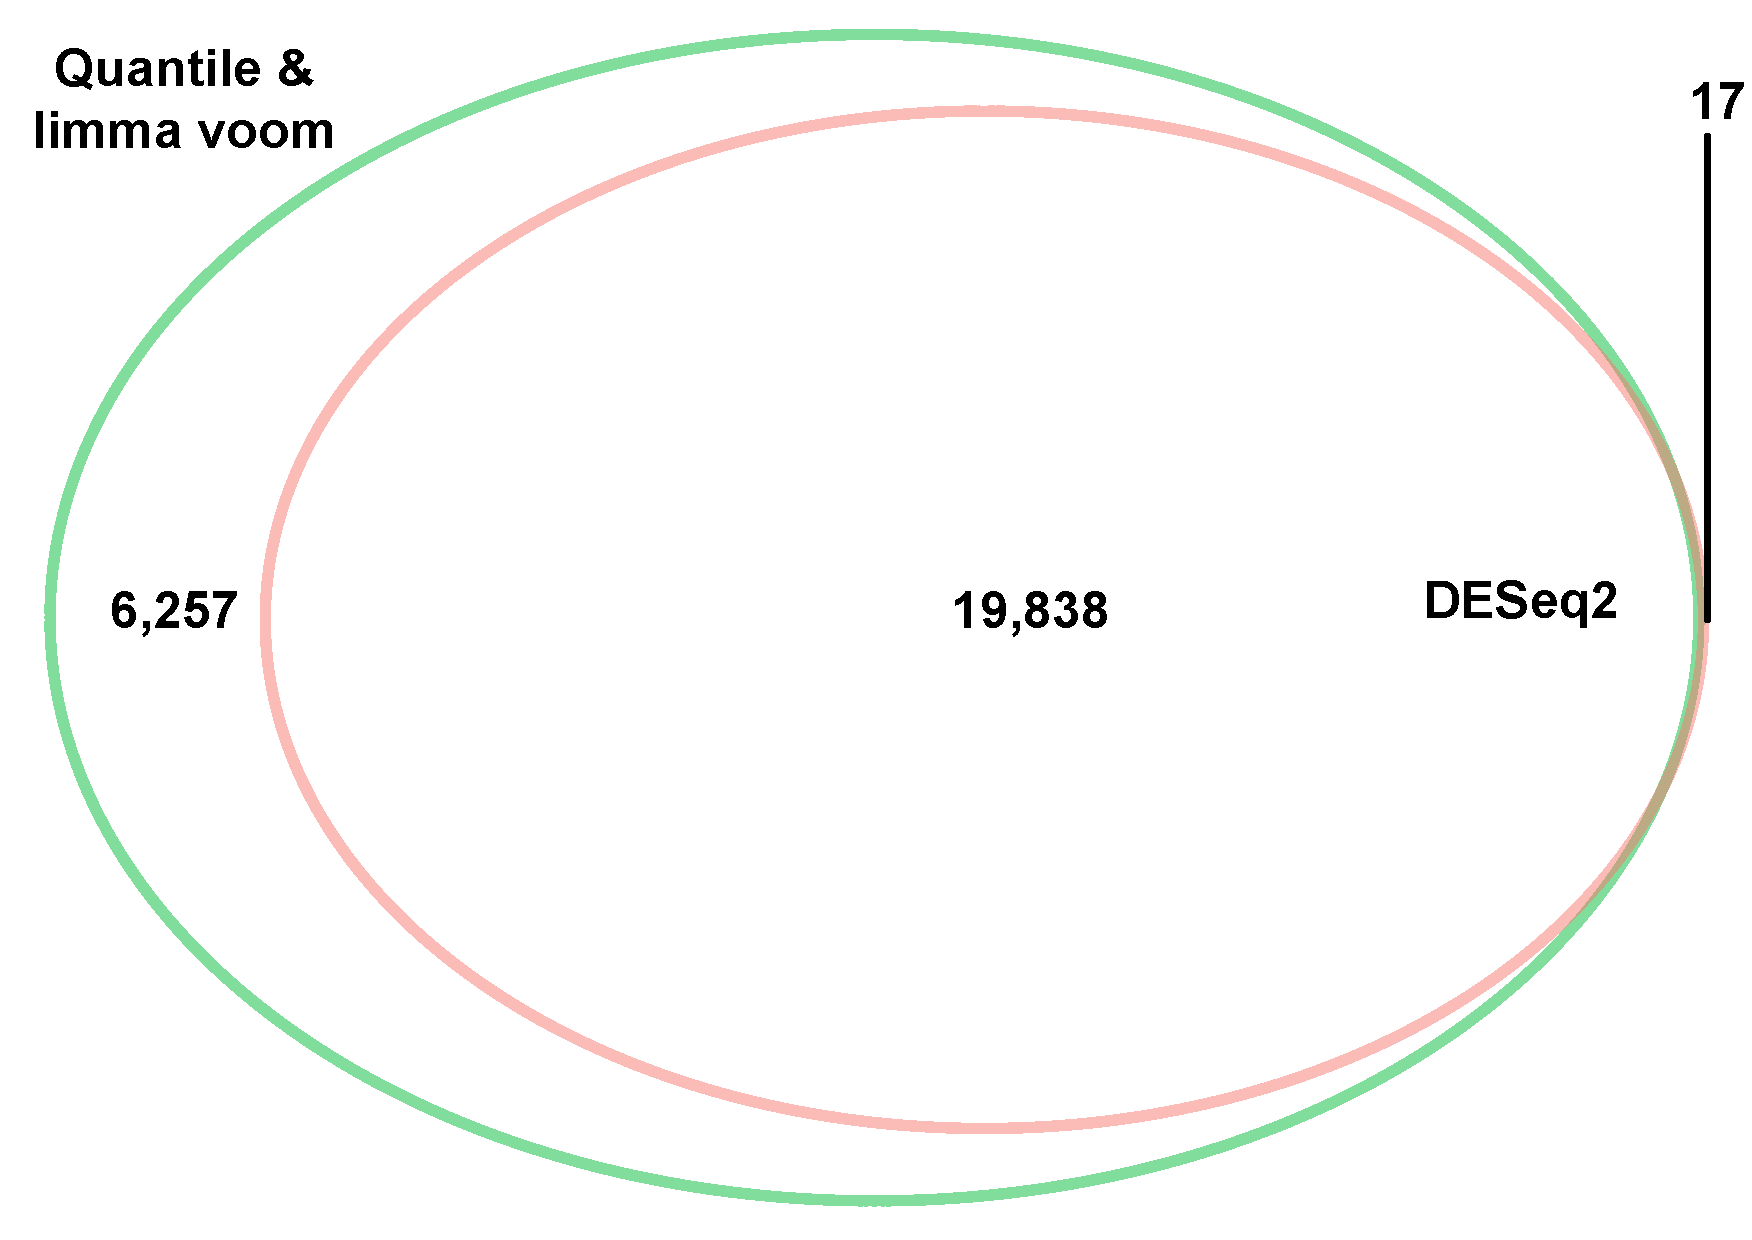
\includegraphics[width=\textwidth]{./Results1/pdfs/ATAC_Core_fresh_CD4vsCD14_venn_diagram_differential_analysis_FDR_01_quantile_DESeq2_only}
\caption{\textbf{}}
\end{subfigure}
\begin{subfigure}{0.5\textwidth}
\centering
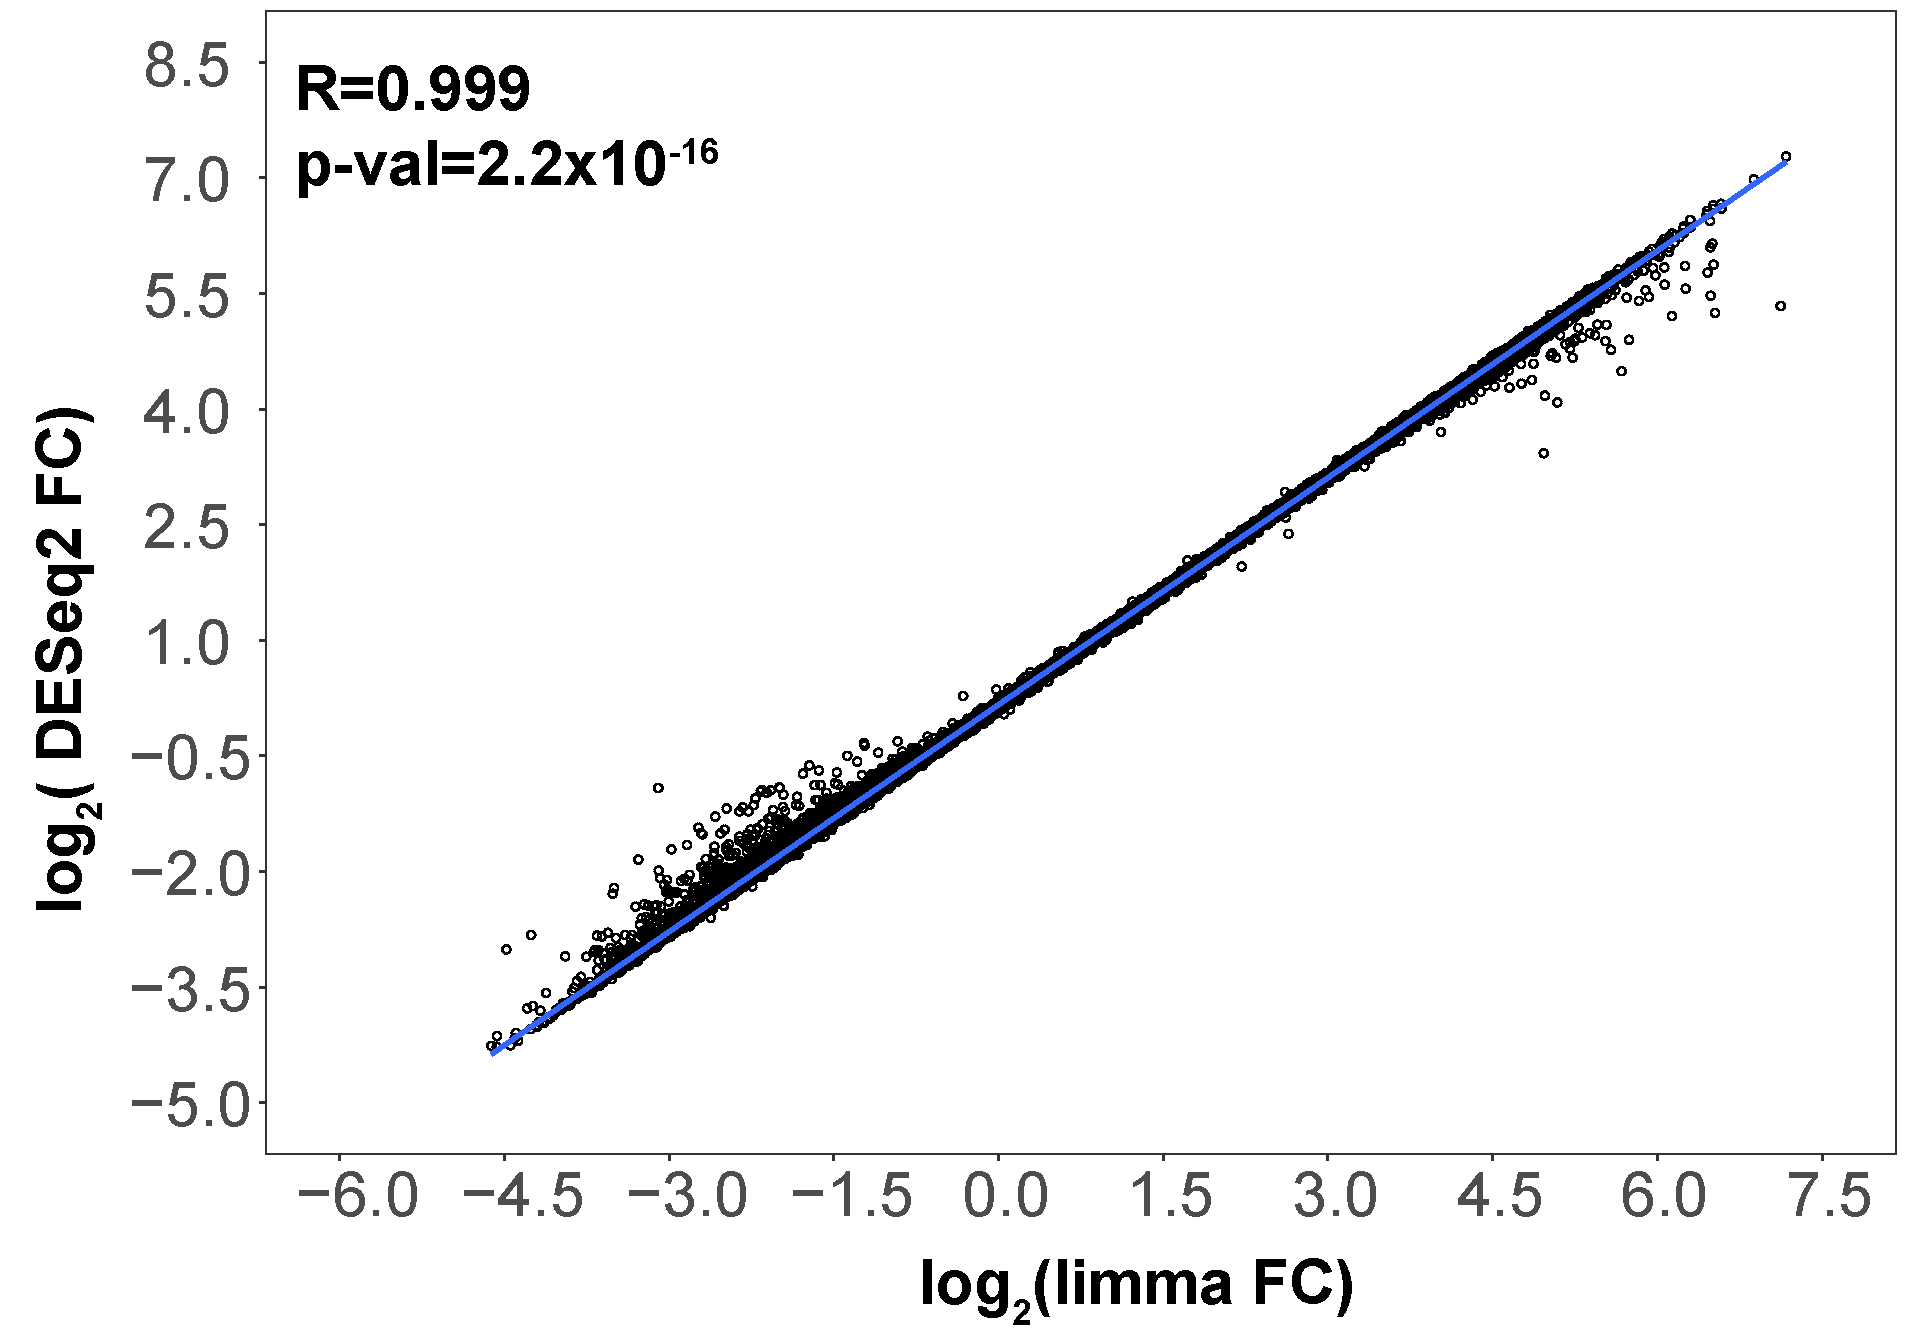
\includegraphics[width=\textwidth]{./Results1/pdfs/ATAC_Core_fastq_CD4_CD14_80pcnt_cut_off_correlation_log2FC_quantile_vs_deseq2}
\caption{\textbf{}} % to add text to the figure name
\end{subfigure}
\caption[Comparison of the DARs identified by differential analysis using limma voom or DESeq for the master list filtered at the optimal cut-off 80\%.]{\textbf{Comparison of the DARs identified by differential analysis using limma voom or DESeq for the master list filtered at the optimal cut-off 80\%.} (A) Venn diagram illustrating the common and distinct significant (FDR$<$0.01 and fold change$>$1.5) DARs identified by differential analysis in the filtered master list for the 80\% optimal cut-off using limma voom or DESeq2. (B) Representation of the correlation between limma voom and DESeq2 log$_2$ fold changes (no FDR filtered) in each the peaks from the filtered master list at the 80\% optimal cut-off. Pearson correlation coefficient (R) and significance (p-value) are indicated. Limma voom was applied to quantile normalised count data.}
\label{figure:QC_quantile_DAR_and_DESeq2_comparison}
\end{figure} 

Lastly, the significant  DARs identified by DESeq2 and filtered for FDR$<$0.01 and fold change$>$1.5 were divided in those more accessible in CD14$^+$ monocytes  (open in monocytes) or CD4$^+$ (open in CD4$^+$). Enrichment analysis for cell type-specific epigenetic features, including FANTOM5 eRNAs, histone marks and DHSs, was conducted in each of the two groups of DARs. The DARs open in CD14$^+$ monocytes included as the top hits for each of the categories T cell eRNAs, CD4$^+$ H3Kme1 and H3K27ac and CD14$^+$ DHSs (Figure \ref{figure:Enrichment_analysis_of_DARs_by_DESeq2}). Conversely, the top enriched features for DARs open in monocytes included eRNAs, H3K27ac and DHSs in monocytes. Overall, this enrichment analysis confirmed the ability of this differential analysis method to identify significant and robust DARs that highlight cell-type specific regulatory regions for CD14$^+$ monocytes and CD4$^+$ cells.


\begin{figure}[htbp]
\centering
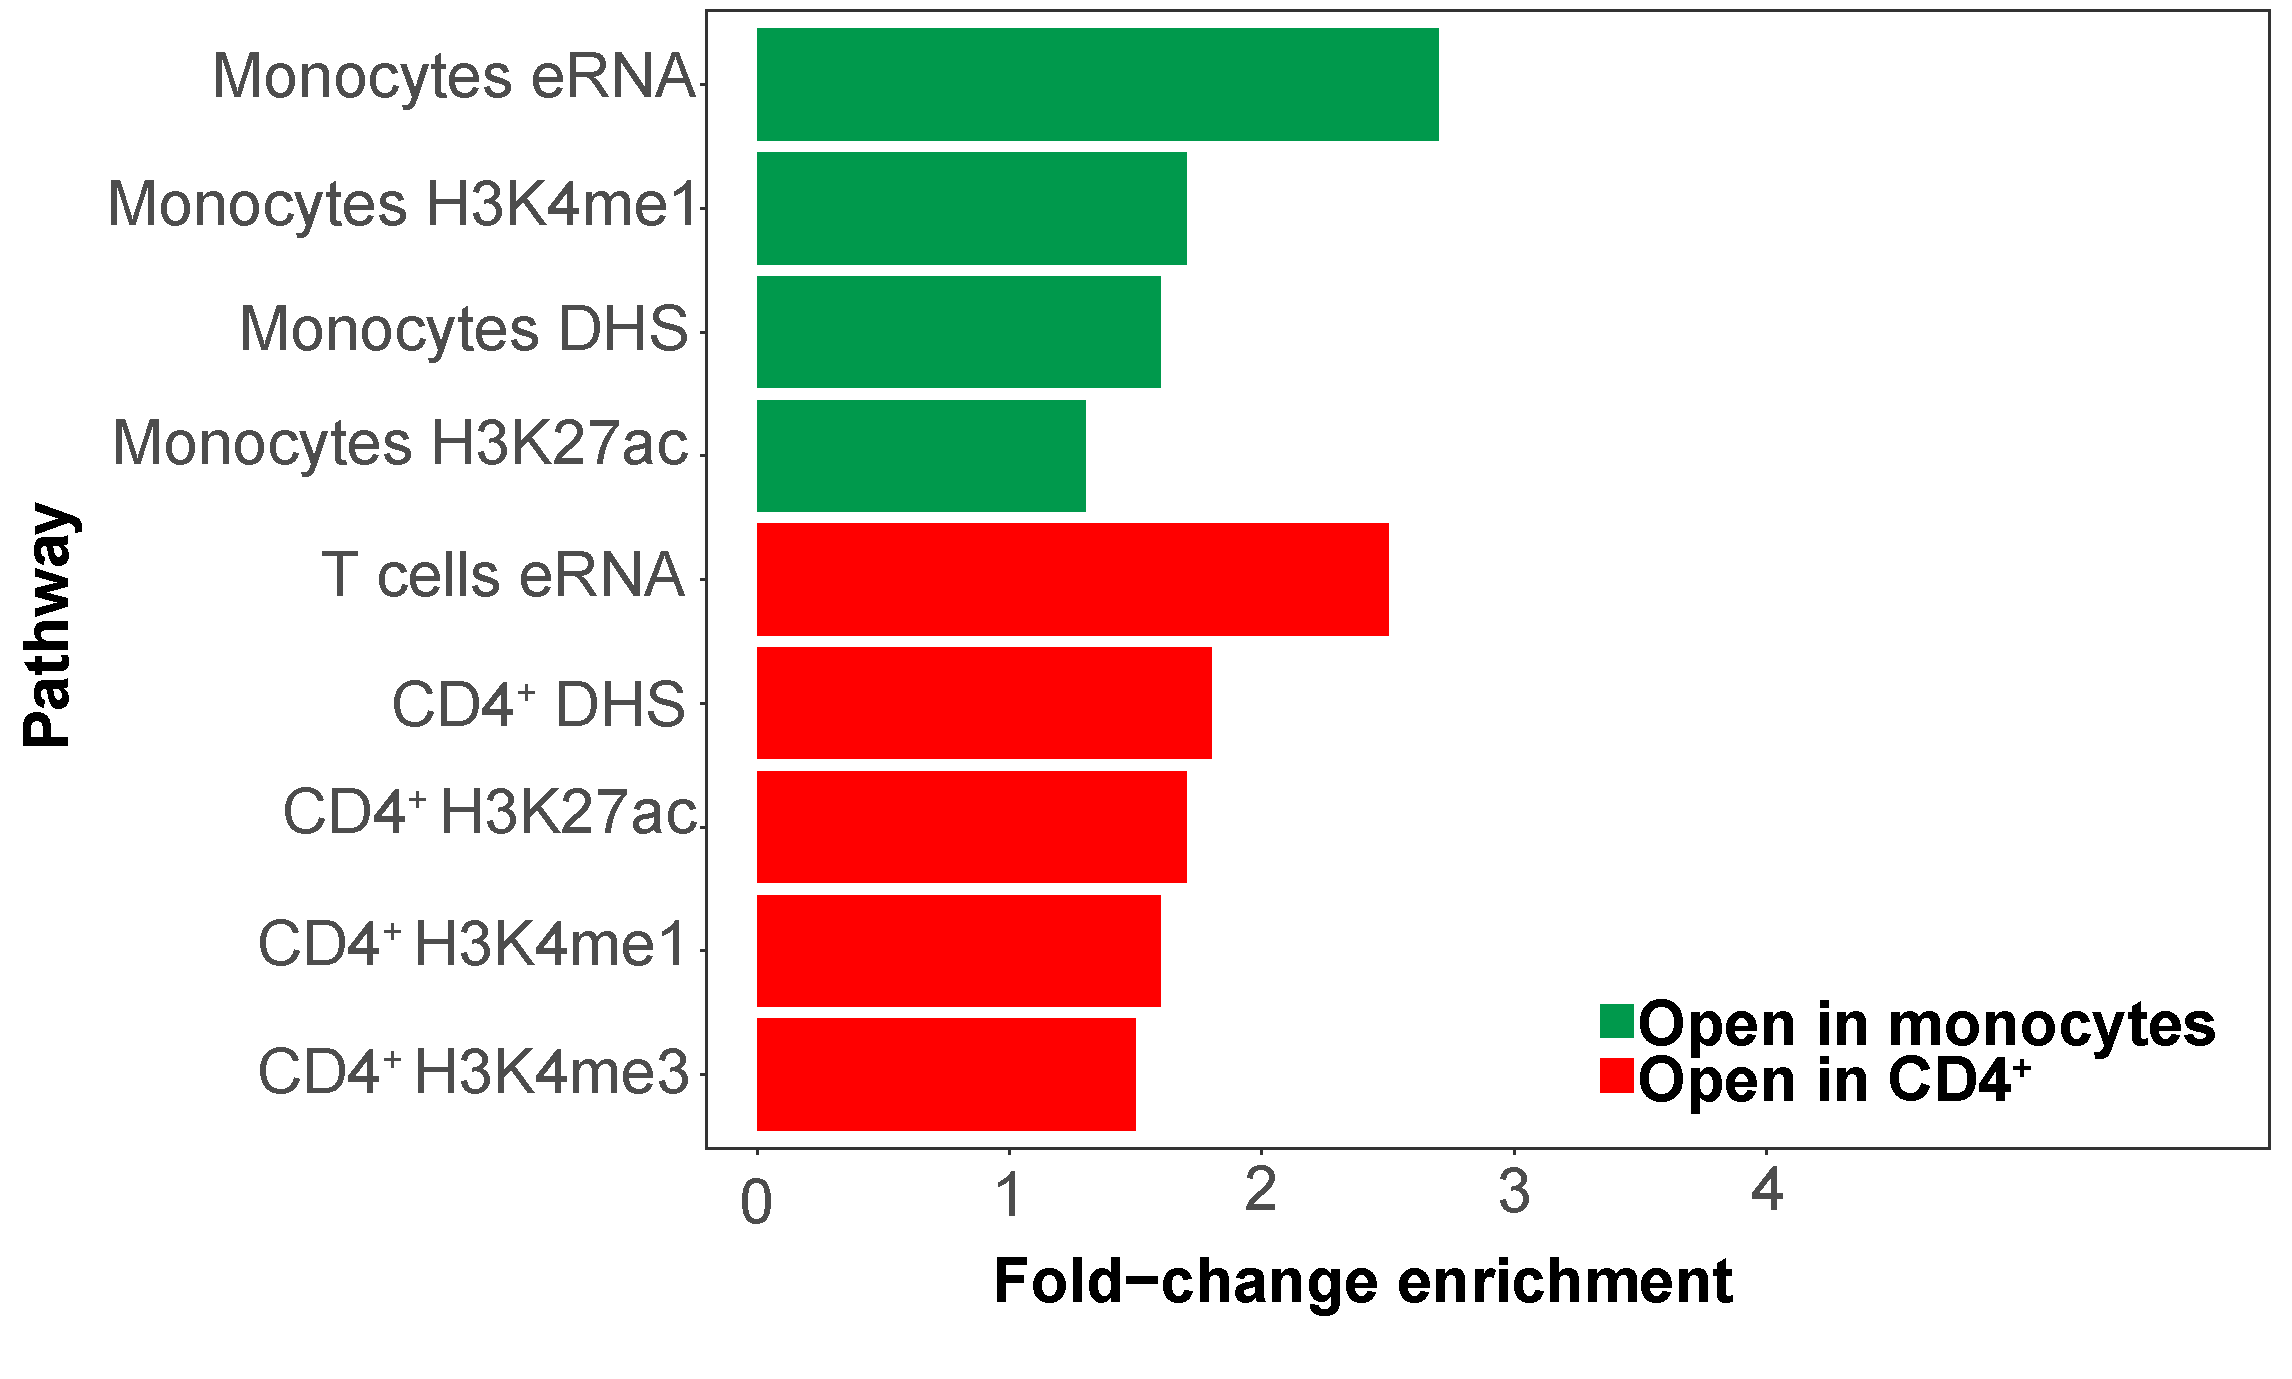
\includegraphics[width=0.6\textwidth]{./Results1/pdfs/ATAC_CD4vsCD14_deseq_features_enrichment_barplot}
\caption[Enrichment analysis for the significant DARs identified by DESeq2 between CD14$^+$ monocytes and CD4$^+$ cells.]{\textbf{Enrichment analysis for the for the significant DARs identified by DESeq2 between CD14$^+$ monocytes and CD4$^+$ cells.} Barplot representing the fold change for the top significantly enriched (FDR$<$0.01) FANTOM5 eRNAs and, histone marks and DHSs from Blueprint. Enrichment analysis was performed separately for the significant (FDR$<$0.01 and fold change$>$1.5) DARs more accessible in CD14$^+$ monocytes (open in monocytes) or CD4$^+$ (open in CD4$^+$).}
\label{figure:Enrichment_analysis_of_DARs_by_DESeq2}
\end{figure} 

%\begin{figure}[htbp]
%\centering
%\begin{subfigure}{0.65\textwidth}
%\centering
%\includegraphics[width=\textwidth]{./Results1/pdfs/ATAC_Core_CD4vsCD14_clusters_and_heatmap_DESeq2_only}
%\caption{\textbf{}}
%\end{subfigure}
%\begin{subfigure}{0.5\textwidth}
%\centering
%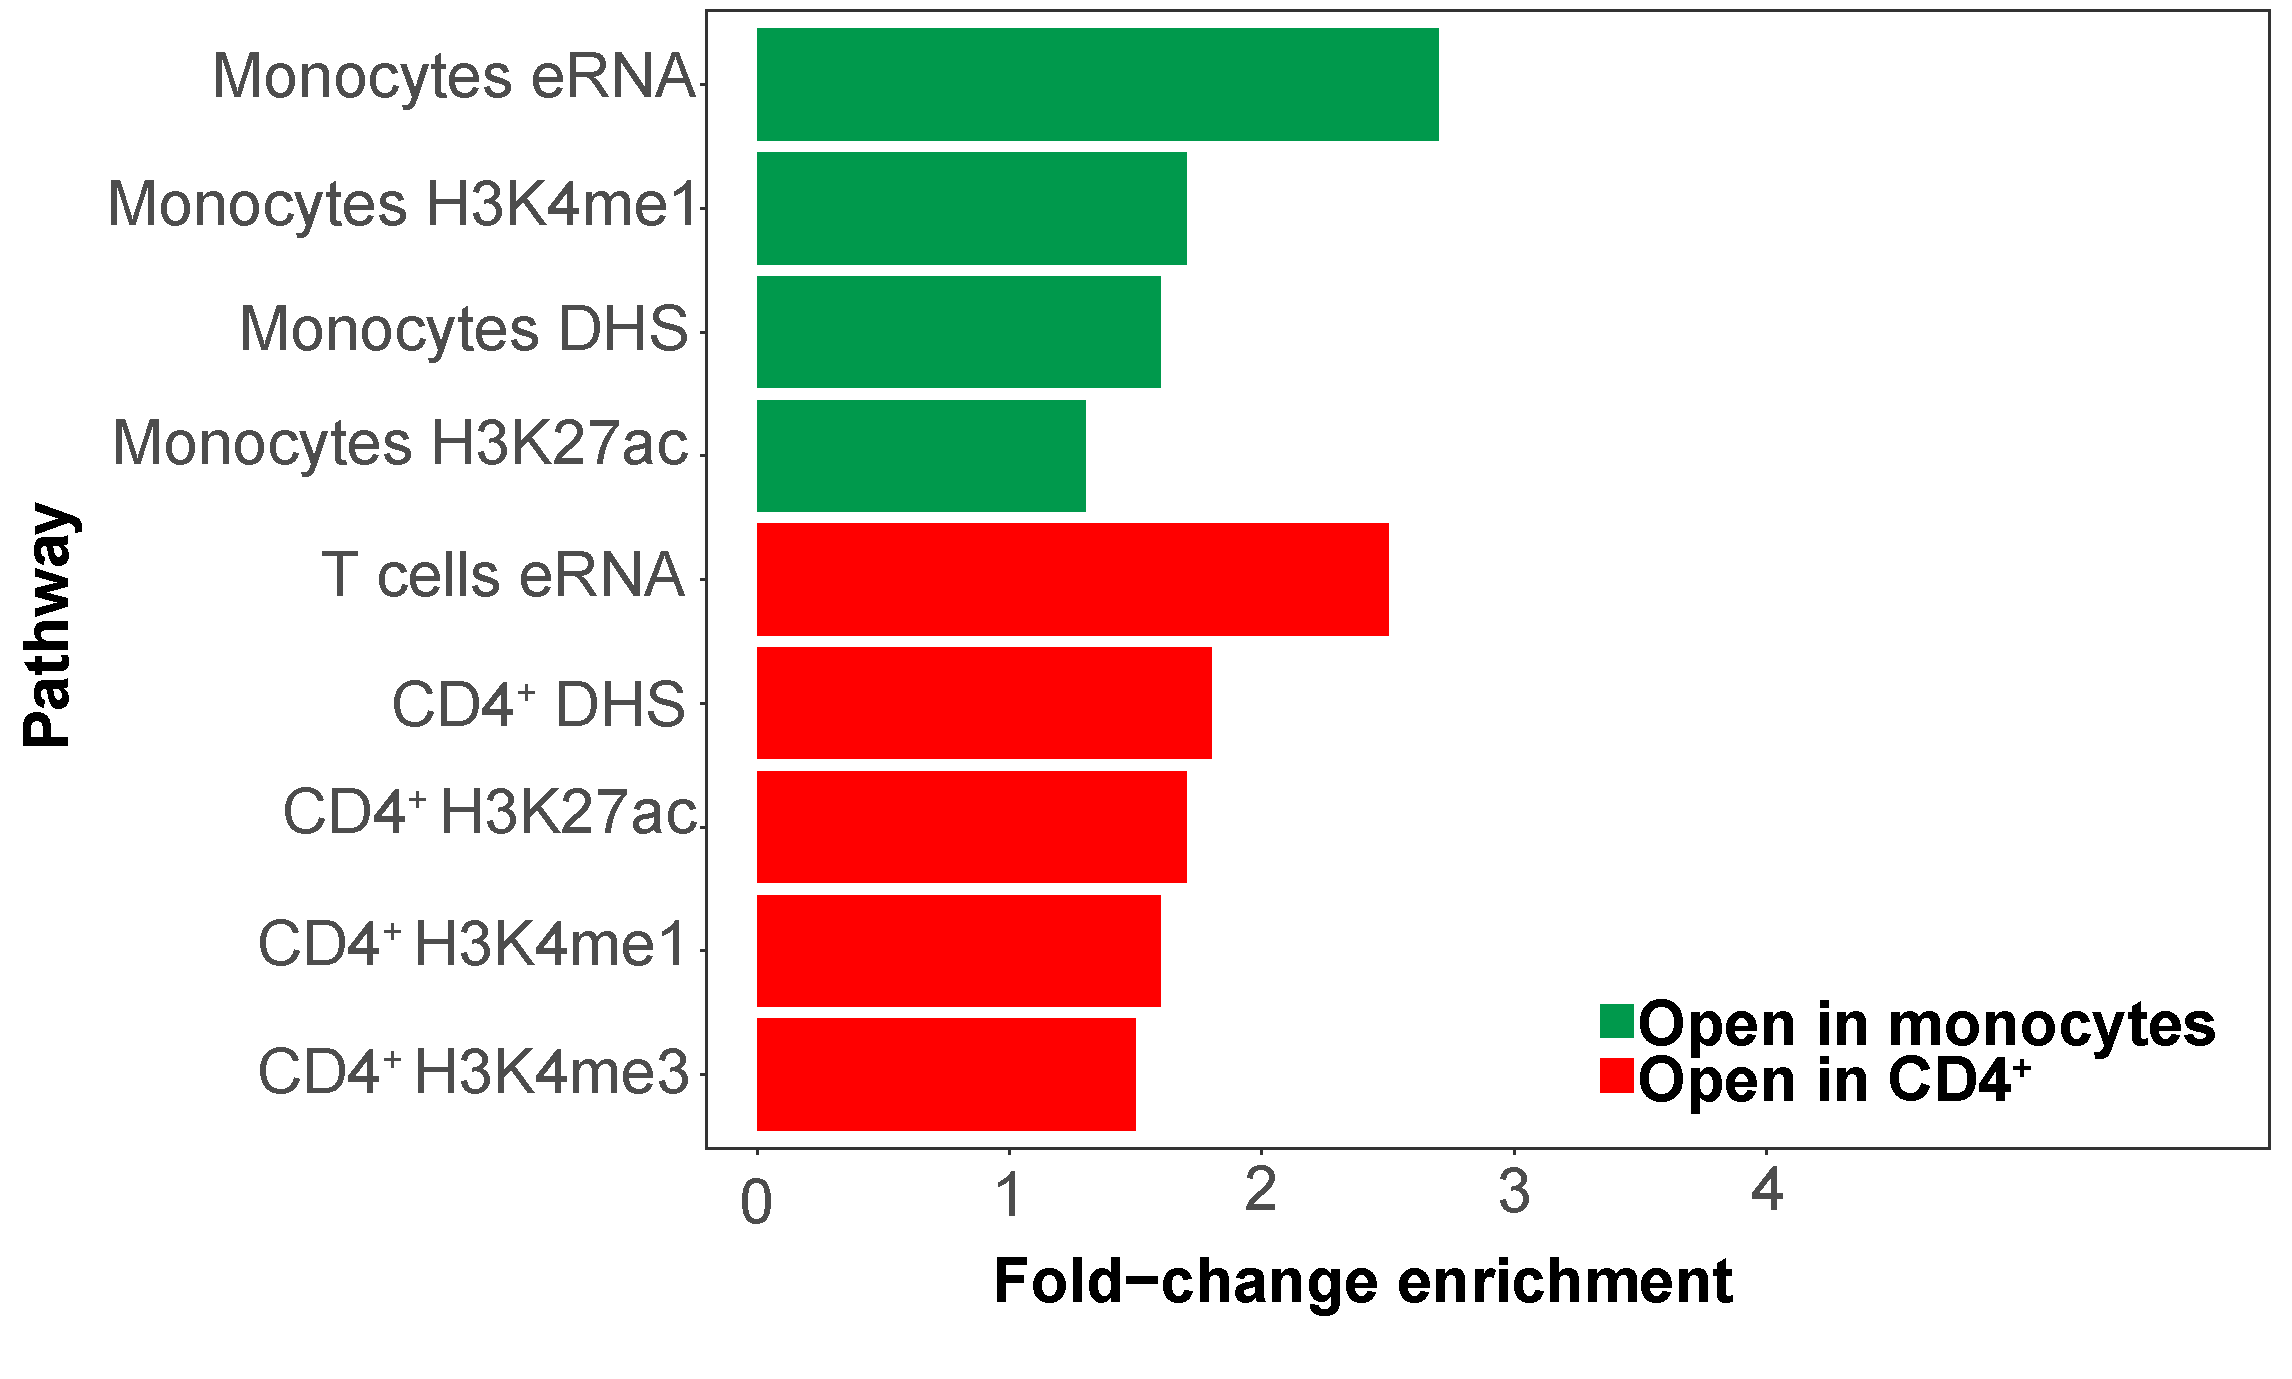
\includegraphics[width=\textwidth]{./Results1/pdfs/ATAC_CD4vsCD14_deseq_features_enrichment_barplot}
%\caption{\textbf{}} % to add text to the figure name
%\end{subfigure}
%\caption[Clustering heatmap and enrichment analysis for the significant DARs identified by DESeq2 between CD14$^+$ monocytes and CD4$^+$ cells.]{\textbf{Clustering heatmap and enrichment analysis for the identified DARs by DESeq2 between CD14$^+$ monocytes and CD4$^+$ cells.} (A)Heatmap showing for each of the ATAC-seq samples included in this analysis, the log$_2$ normalised counts at each of the 19,838 significant (FDR$<$0.01 and abs(fold change)$>$1.5) DARs identified by DESeq2. Each row represents a DAR and are clustered based on DARs presenting similar patterns of accessibility in each of the three replicates for the two cell types compared. (B) Barplot representing the fold change for the top significantly enriched (FDR$<$0.01) FANTOM5 eRNAs and Blueprint histone marks and DHSs.}
%\label{figure:Heatmap_and_enrichment_analysis_of_DARs_by_DESeq2}
%\end{figure} 
%



\subsection{Assessment of ATAC-seq transposition times in relevant cell types}
\label{ATACseq}

The duration of the transposition reaction was optimised for the main immune cell types of interest for this thesis. ATAC-seq was performed for three different transposition times (20, 30 and 40 min) in CD14$^+$ monocytes, CD4$^+$, total CD8$^+$ (CD8$^+$) and CD19$^+$ cells in one healthy control sample included in cohort 1A from Chapter \ref{ch:Results2} (Tables \ref{tab:Summary_all_cohorts} and \ref{tab:Control_cohort_metadata}). The impact of transposition time on various ATAC-related readouts was explored. All three transpostion times produced appropriate fragment size distributions which recapitulated the nucleosome periodicity pattern (Figure \ref{figure:Transposition_times_ATAC}A). The duration of the transposition time is known to have an effect on the proportion of nucleosome-free and nucleosome-bound (mono-nucleosomes and beyond) regions tagged by the adapters. Ideally, the transposition reaction should maximise NFF ($\leq$150bp), where TF and other proteins bind. In order to explore this effect in the different cell types, the ratio between NFF and nucleosome-bound fragments (NBF) ($>$150bp) was calculated (Figure \ref{figure:Transposition_times_ATAC}B). The relationship of this ratio with transposition time was heterogenous between cell types. For example, CD8$^+$ presented the greatest proportion of NFR for 20 min of transposition whereas the NFF/NBF reached a maximum at 40 min for the CD14$^+$ monocytes. However, the change in this ratio across transposition times was very moderate in all cell types but CD8$^+$ cells. 


\begin{figure}[htbp]
\centering
\begin{subfigure}{0.5\textwidth}
\centering
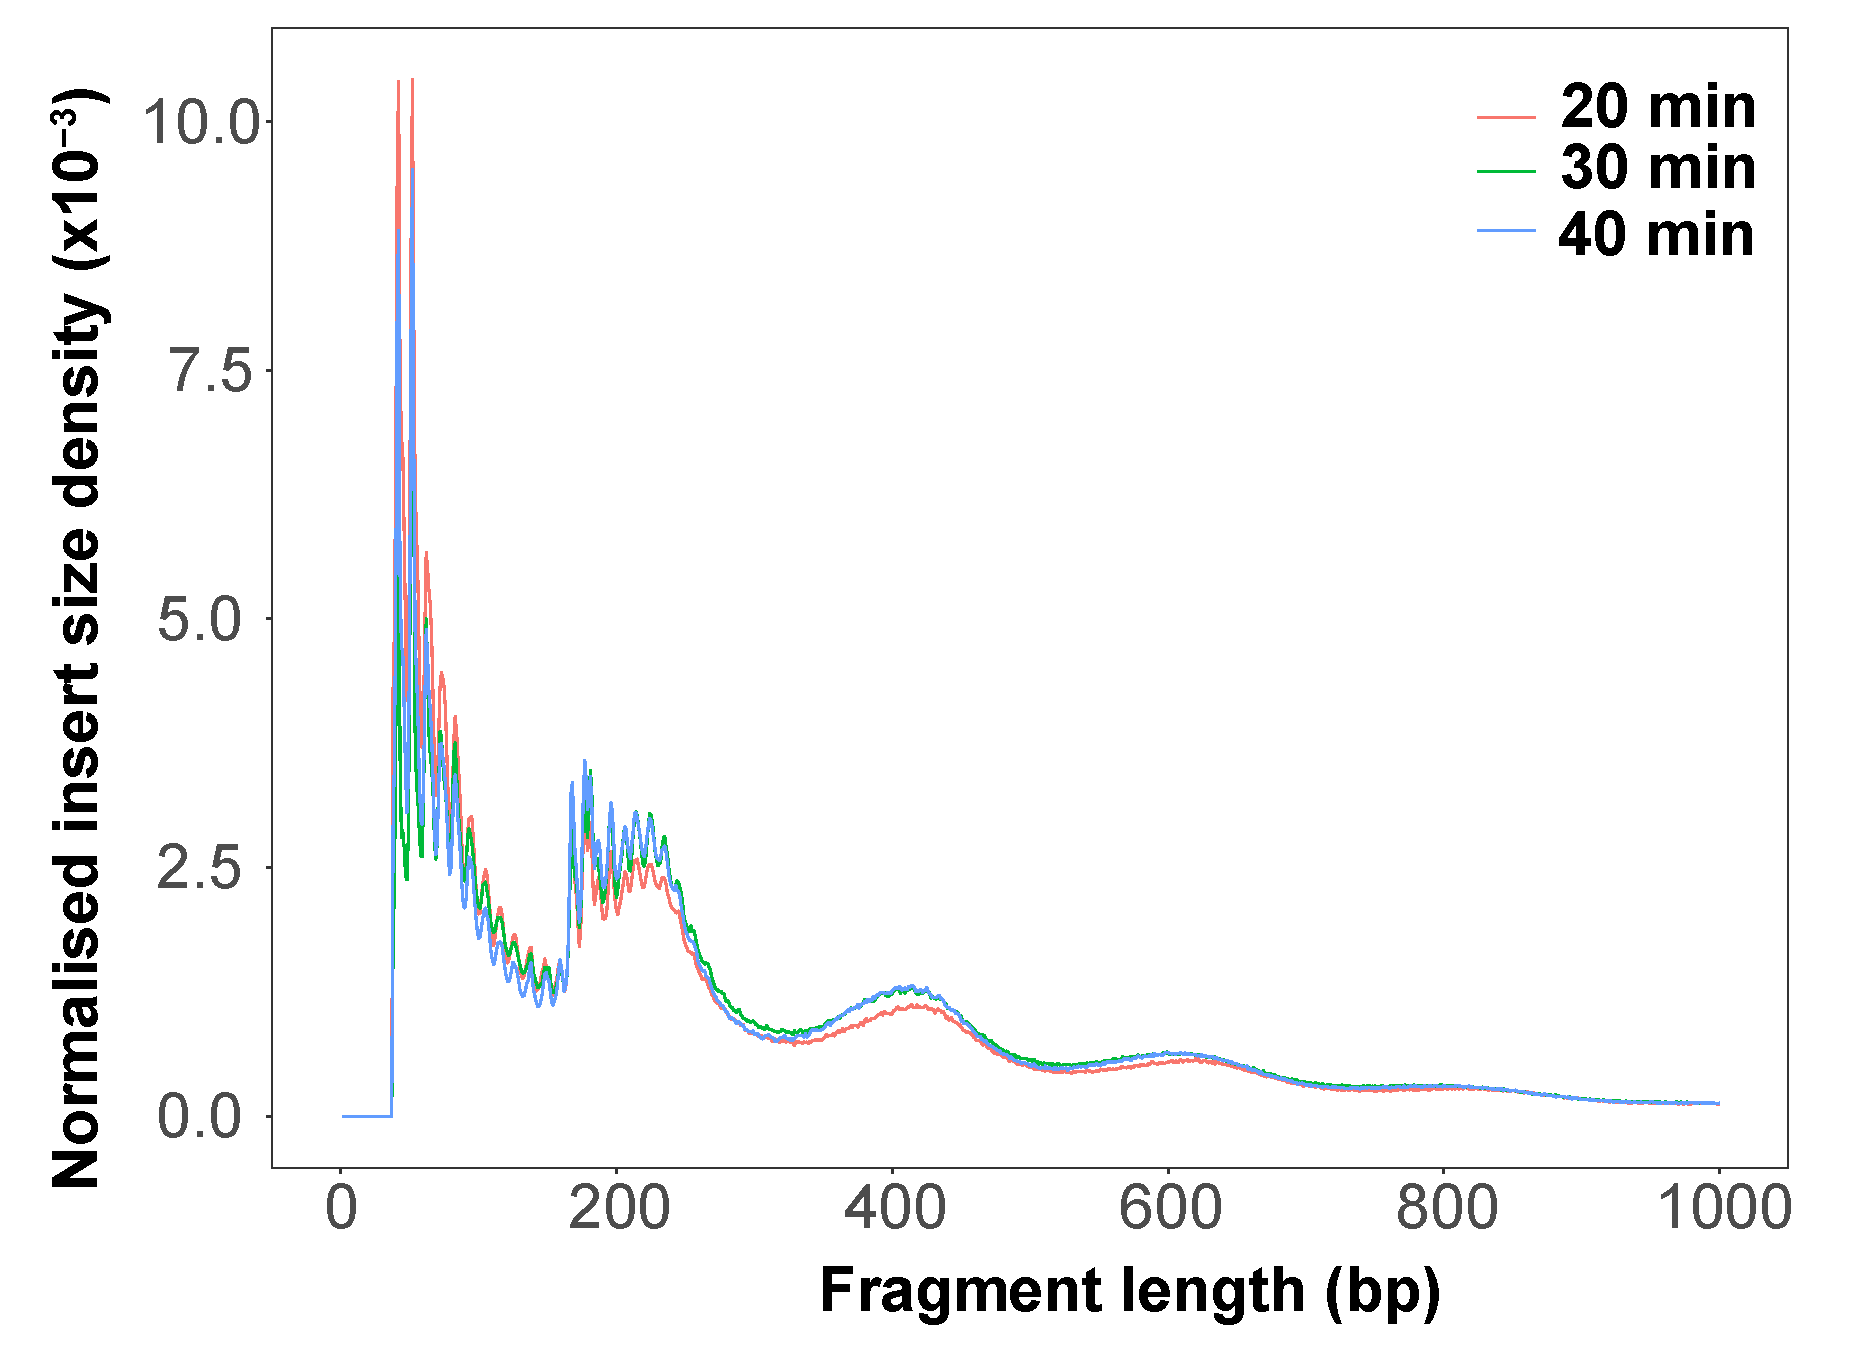
\includegraphics[width=\textwidth]{./Results1/pdfs/ATAC_CD8_fragment_size_distribution_20_30_40min}
\caption{\textbf{}}
% The percentage sign indicated that the other subfig goes side by side
\end{subfigure}%
\begin{subfigure}{0.5\textwidth}
\centering
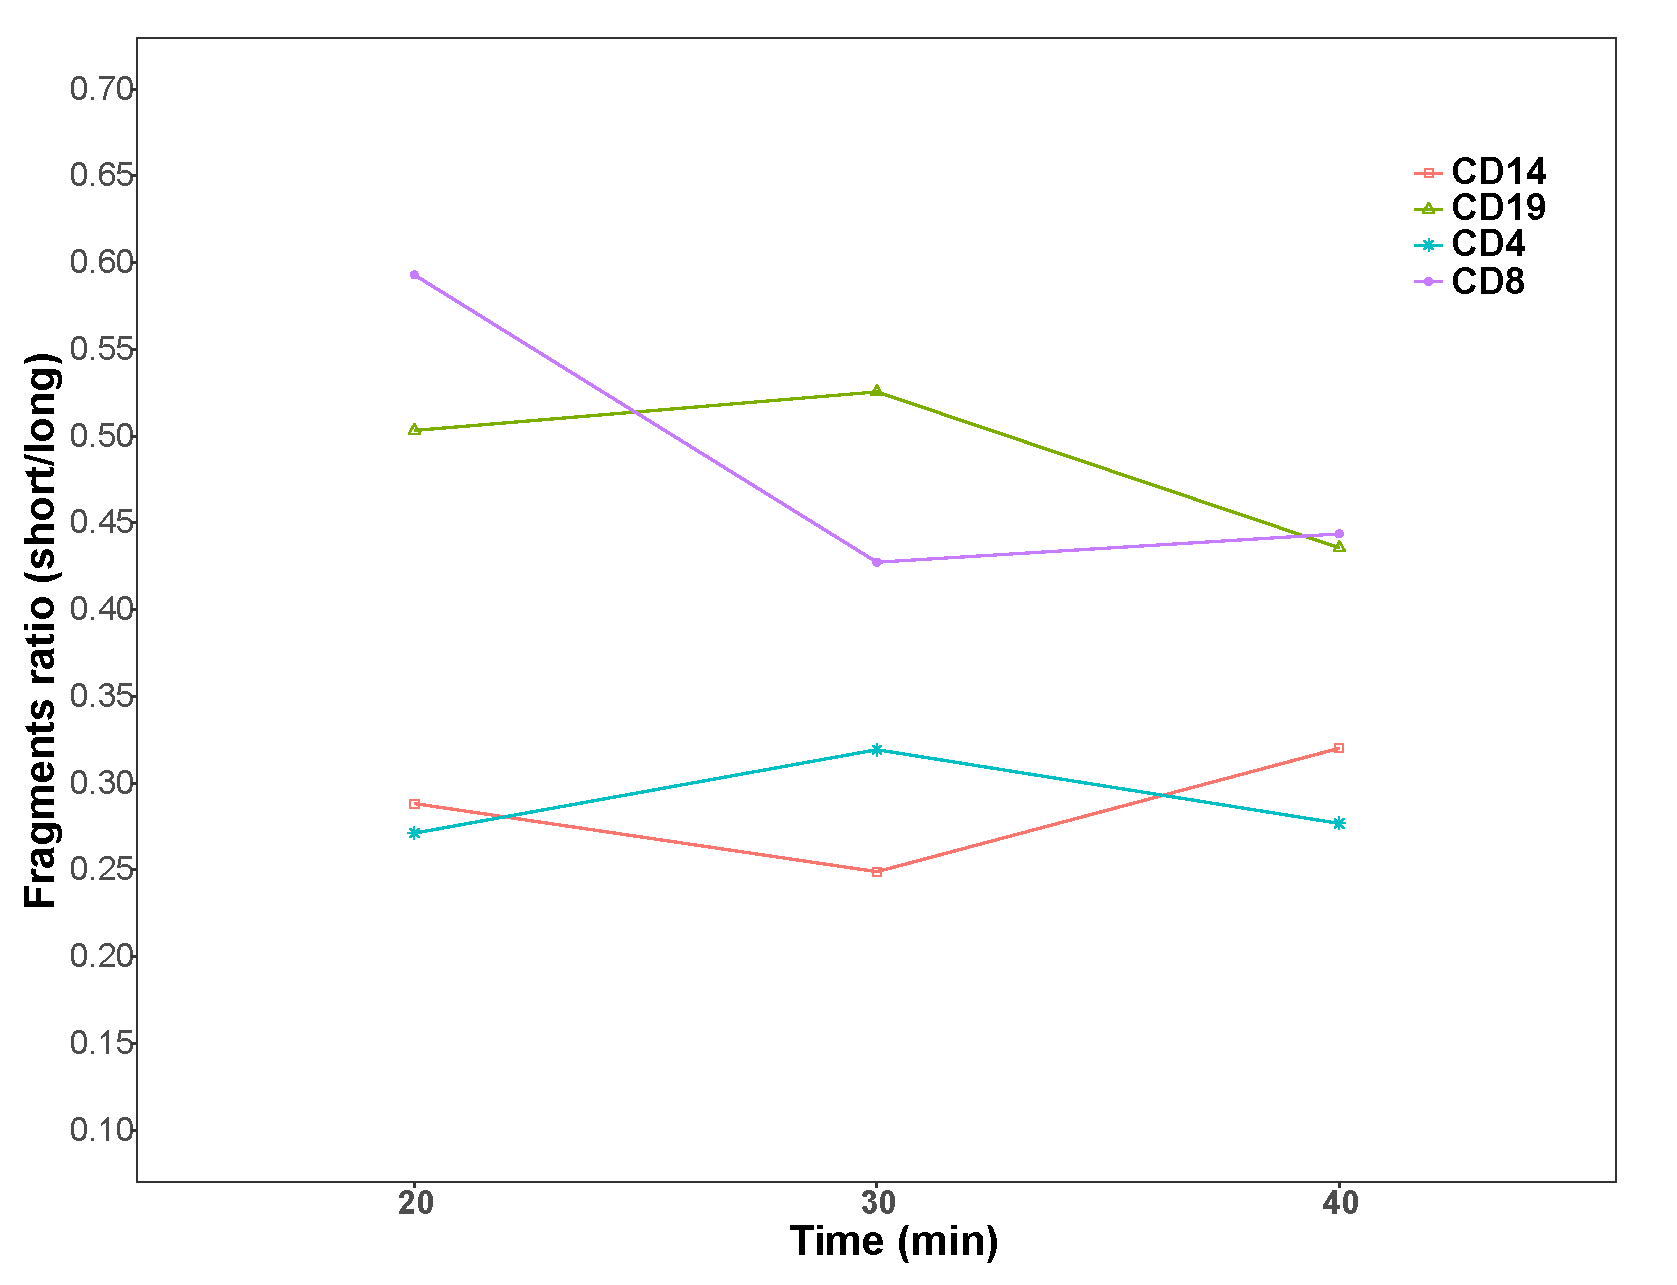
\includegraphics[width=\textwidth]{./Results1/pdfs/ATAC_ratio_short_long_fragments_20_30_40_min}
\caption{\textbf{}}
\end{subfigure} \\
\begin{subfigure}{0.5\textwidth}
\centering
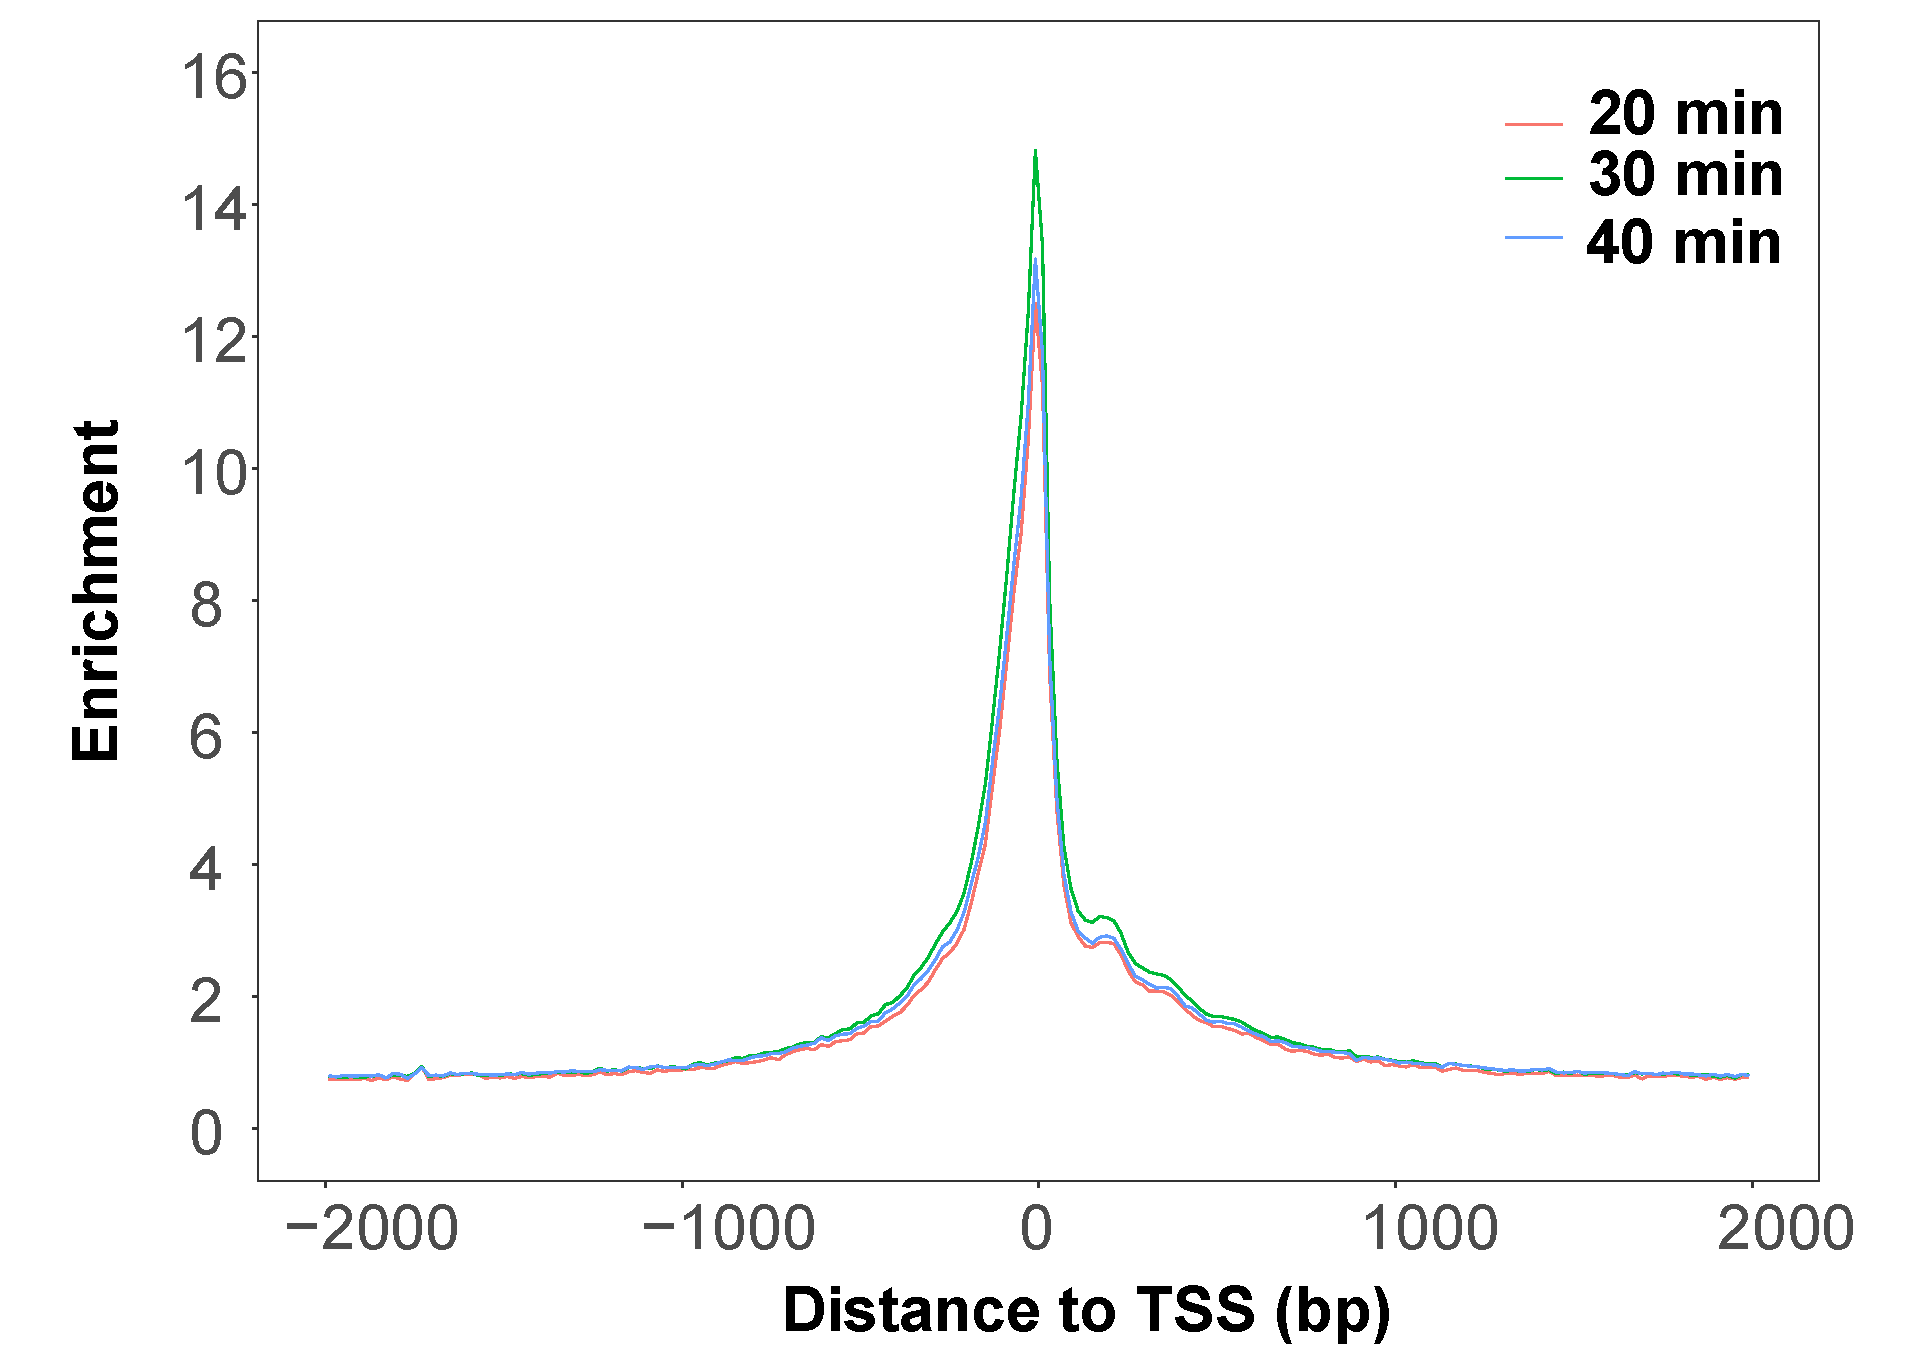
\includegraphics[width=\textwidth]{./Results1/pdfs/ATAC_optimisation_CD4_20_30_40_min_tss_enrichment}
\caption{\textbf{}} % to add text to the figure name
\end{subfigure}
\caption[Assessment of the effect of transposition times on the ATAC-seq measurements]{\textbf{Assessment of the effect of transposition times on the ATAC-seq measurements}. (A) Representative plot of the ATAC-seq fragment sizes density distribution following 20, 30 and 40 min of transposition in healthy total CD8$^+$ cells. (B) Changes in the ratio between nucleosome-free fragments (NFF) (fragments $\leq$150bp) and long ($>$151bp) ATAC-seq nucleosome-bound fragments (NBF) across different transposition times in CD14$^+$ monocytes, CD4$^+$, CD8$^+$ and CD19$^+$ cells.}
\label{figure:Transposition_times_ATAC}
\end{figure} 

Transposition times did not significantly affect the signal-to-noise ratio measured as fold-enrichment at the TSS, with the largest enrichment values corresponding to different times across the four cell types (Figure \ref{figure:Transposition_times_ATAC}C). For all cell types, 30 and 40 min yielded the ATAC-seq libraries with the largest enrichment, with the differences between the two being very modest (not more than 4 units difference) across all cell types (data not shown). Before performing this formal comparison of transposition times, some sample recruitment had already been conducted using ATAC-seq with transposition for 40 min, as it was found to be the most appropriate condition based on the relative abundance of DNA fragment sizes profiles from the pre-sequencing library quality control (here not shown). Although this analysis suggests 30 min is the best condition for most of the cell types tested, the differences between 30 min and 40 min were minor and therefore for consistency across the cohort 40 min was used for all other patient samples using ATAC-seq. 



\subsection{Comparison of ATAC-seq with Fast-ATAC protocol}
\label{Fast_ATAC}

An improved Fast-ATAC protocol from Corces and colleagues \parencite{Corces2016} was reported during the time the work in this thesis was being undertaken and was compared with the ATAC-seq protocol from Buesnrostro and colleagues \parencite{Buenrostro2013}, which was being used at the time to generate some of the data in this thesis. The aim was to confirm the two main reported advantages of Fast-ATAC, namely reduction of mitochondrial reads and signal enhancement, before implementing it as the replacement for the ATAC-seq protocol, which had been being used for processing patient and control samples (Chapter \ref{ch:Results2} cohort 1A in Tables \ref{tab:Summary_all_cohorts}, \ref{tab:Psoriasis_cohort_metadata} and \ref{tab:Control_cohort_metadata}). Fast-ATAC was conducted in one healthy volunteer sample included in cohort 1B from Chapter \ref{ch:Results2} (Tables \ref{tab:Summary_all_cohorts} and \ref{tab:Control_cohort_metadata}). Fast-ATAC, as previously mentioned was specifically optimised for hematopoietic cells and used 30 min of transposition. Thus, for consistency, Fast-ATAC samples were here compared to the ATAC-seq library from \label{ATACseq} transposed for 30 min in the same 4 cell types.

The percentage of mitochondrial reads in the Fast-ATAC libraries was lower for all cell types analysed compared to ATAC-seq (Figure \ref{figure:ATAC_vs_FAST_ATAC}A). Importantly, the mitochondrial percentage in CD4$^+$ and CD8$^+$ cells showed a reduction from 50\% to less than 20\%. With regard to the background signal, differing trends were observed across cell types (Figure \ref{figure:ATAC_vs_FAST_ATAC}B) with no change in TSS enrichment for CD14$^+$ monocytes or CD4$^+$ T cells while CD8$^+$ and CD19$^+$ cells showed a reduction with Fast-ATAC when compared to ATAC-seq. Overall, the large decrease in mitochondrial reads together with the reduced duration of the experimental protocol supported the replacement of ATAC-seq by Fast-ATAC for future patient recruitments (see Chapter \ref{Results2}). 



\begin{figure}[htbp]
\centering
\begin{subfigure}{0.5\textwidth}
\centering
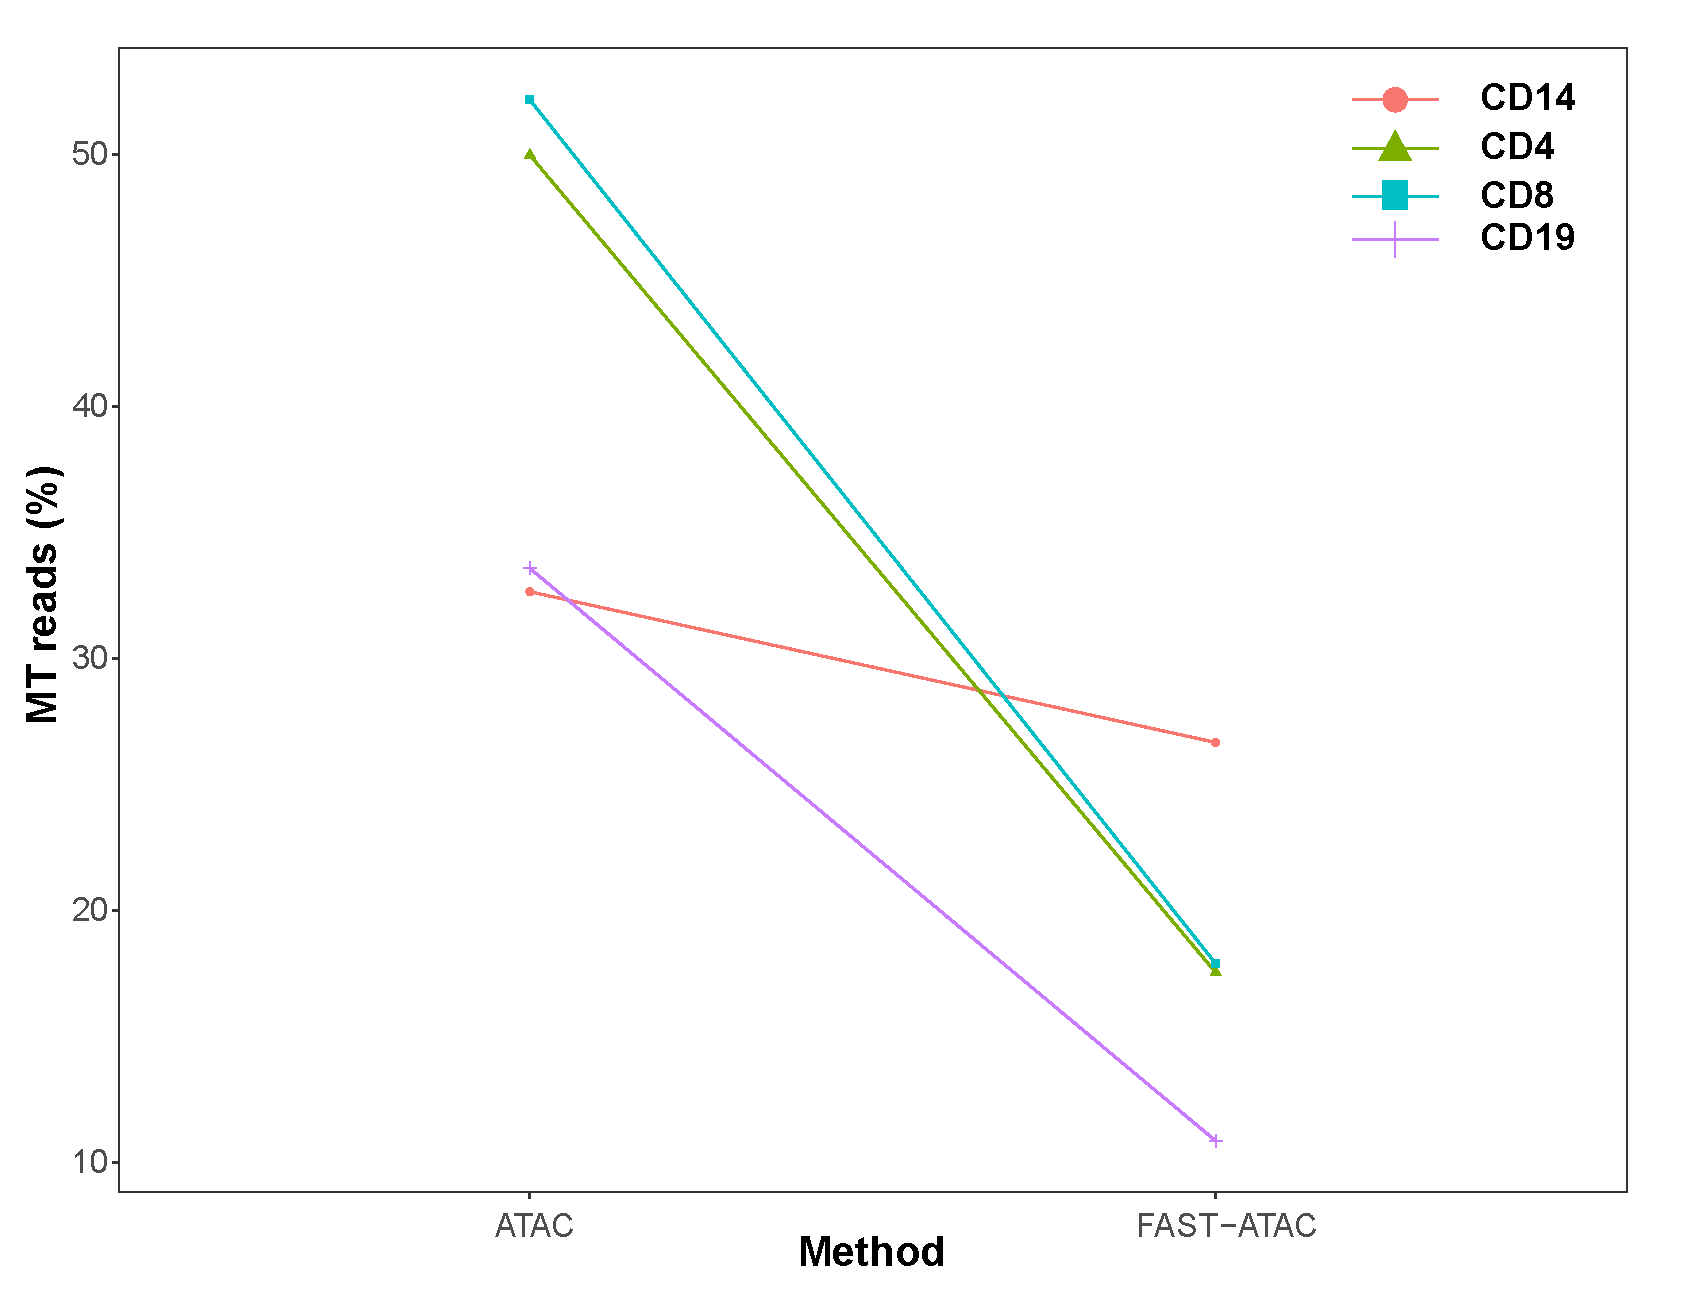
\includegraphics[width=\textwidth]{./Results1/pdfs/ATAC_vs_FAST_ATAC_percnt_MT_reads_dotplot}
\caption{\textbf{}}
% The percentage sign indicated that the other subfig goes side by side
\end{subfigure}%
\begin{subfigure}{0.5\textwidth}
\centering
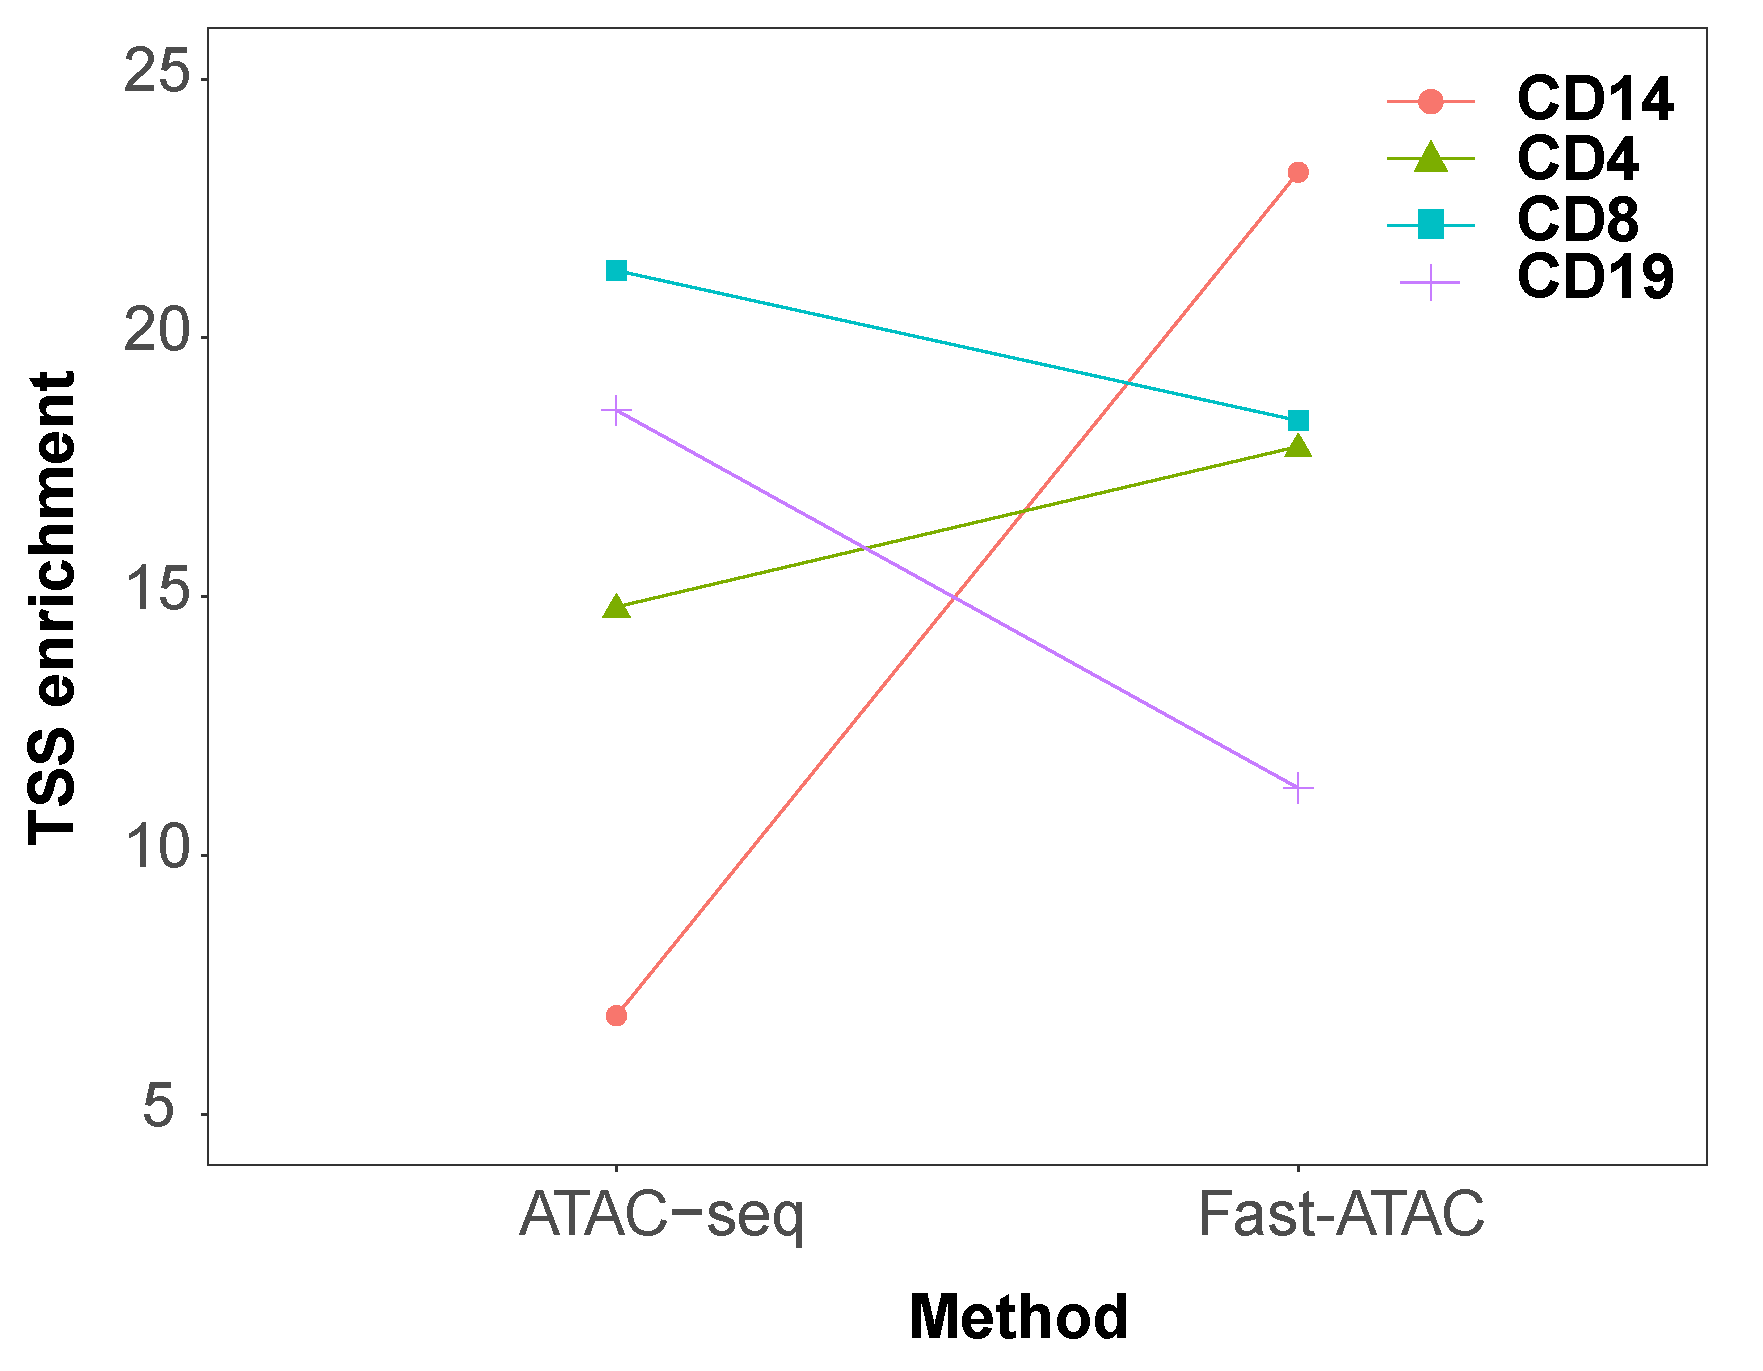
\includegraphics[width=\textwidth]{./Results1/pdfs/ATAC_vs_FAST_ATAC_tss_dotplot}
\caption{\textbf{}}
\end{subfigure}
\caption[Differences in mitochondrial DNA abundance and TSS enrichment between ATAC-seq and Fast-ATAC protocols.]{\textbf{Differences in mitochondrial DNA abundance and TSS enrichment between ATAC-seq and Fast-ATAC protocols.} Representation of changes in (A) percentage of mitochondrial reads and (B) TSS fold-enrichment between ATAC-seq and Fast-ATAC libraries for CD14$^+$ monocytes, CD4$^+$, CD8$^+$ and CD19$^+$ cells. Fast-ATAC protocol was specifically optimised by Corces and colleagues for hematopoietic cells and recommends 30 min of tranposition (\ref{ch:Mat} and Corces \textit{et al.}, 2016). Therefore, for consistency, Fast-ATAC samples were compared to the ATAC-seq libraries from \ref{ATACseq} transposed for 30 min.}
\label{figure:ATAC_vs_FAST_ATAC}
\end{figure} 



\subsection{Limitations of ATAC-seq and Fast-ATAC to assess chromatin accessibility in keratinocytes}
A particular aim of this thesis was to characterise the regulatory landscape in keratinocytes, one of the most relevant cell types in psoriasis pathophysiology. In order to assess the feasibility of using the ATAC-seq protocol from Buenrostro and colleagues \parencite{Buenrostro2013} (referred to ATAC 1 in this subsection), the epidermis was isolated from a psoriatic lesional skin biopsy, digested with trypsin and filtered through a cell strainer to ensure a single-cell suspension, as detailed in Chapter \ref{ch:Mat}. Approximately 50,000 cells from the suspension were counted and ATAC 1 was performed for two different transposition times (30 and 40 min). Since biopsy handling and lesional epidermal keratinocytes are particularly challenging, this was considered the best system to test the performance of the standard protocol in the clinical setting of interest for the study. Library quality control based on pre-sequencing profiles of relative abundance of DNA library fragment sizes for the two samples revealed expected DNA fragment sizes that recapitulated the characteristic nucleosome pattern every $\sim$200bp generated by transposition of nucleosome-free and nucleosome-bound DNA (Figures \ref{figure:PS02_skin_ATAC_QC_assessment}A and \ref{figure:PS2_40min_tapestation}). This was consistent with the fragment size distribution from the NGS data, presenting NFF and NBF (mono-and di-nuclosomes only) for both transposition times (Figure \ref{figure:PS02_skin_ATAC_QC_assessment}B). However the relative abundance of the mono-nucleosome fragments appeared to be approximately equal to the NFF, which is not observed in higher quality libraries. Regarding the signal-to-noise ratio, libraries for both transposition times presented TSS fold enrichment below the acceptable cut-off threshold of 6, showing slightly better signal (3.5 fold-enrichment) in the 30 min library (Figure \ref{figure:PS02_skin_ATAC_QC_assessment}C). Cell suspensions obtained from skin biopsies using trypsinisation of the epidermal layer are enriched in keratinocytes, constituting approximately 90\% of the cells \parencite{Haftek1986}. However, dead cells and free-DNA released by apoptotic cells throughout processing could contribute to the increased background noise observed above. 



\begin{figure}[htbp]
\centering
\begin{subfigure}{0.7\textwidth}
\centering
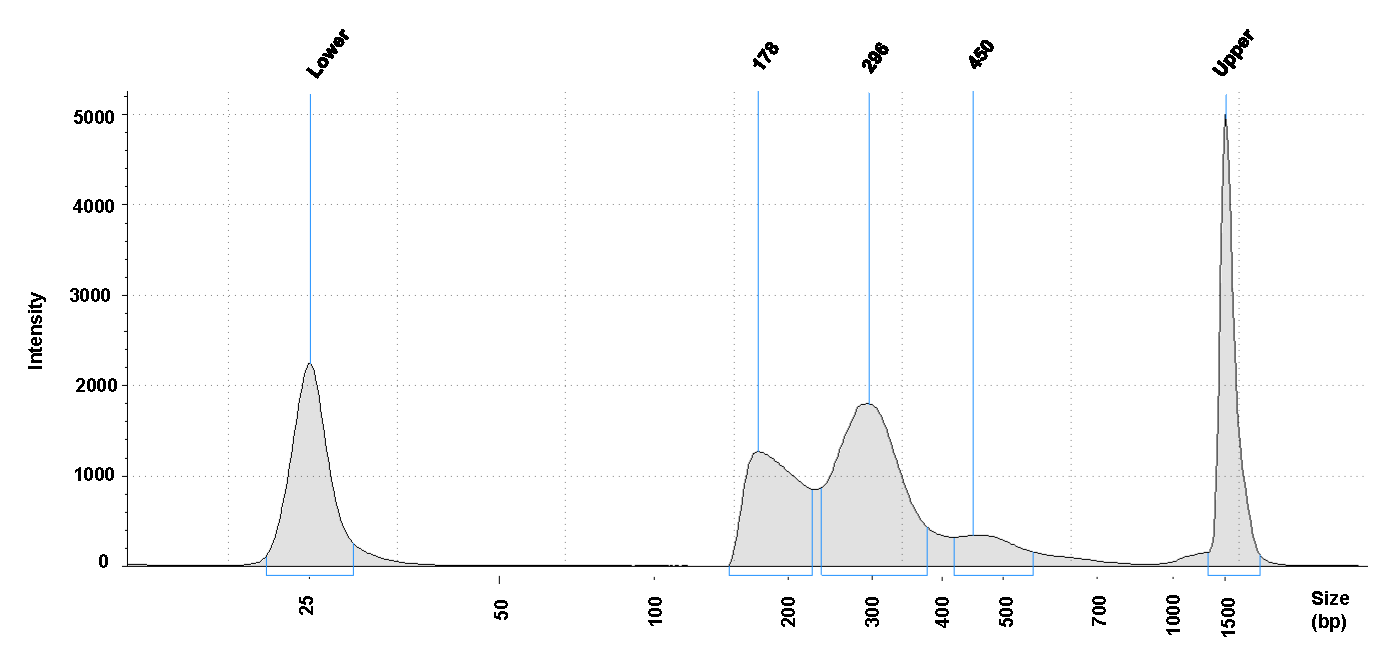
\includegraphics[width=\textwidth]{./Results1/pdfs/ATAC_PS02_tapestation_30min}
\caption{\textbf{}}
\end{subfigure}
\begin{subfigure}{0.45\textwidth}
\centering
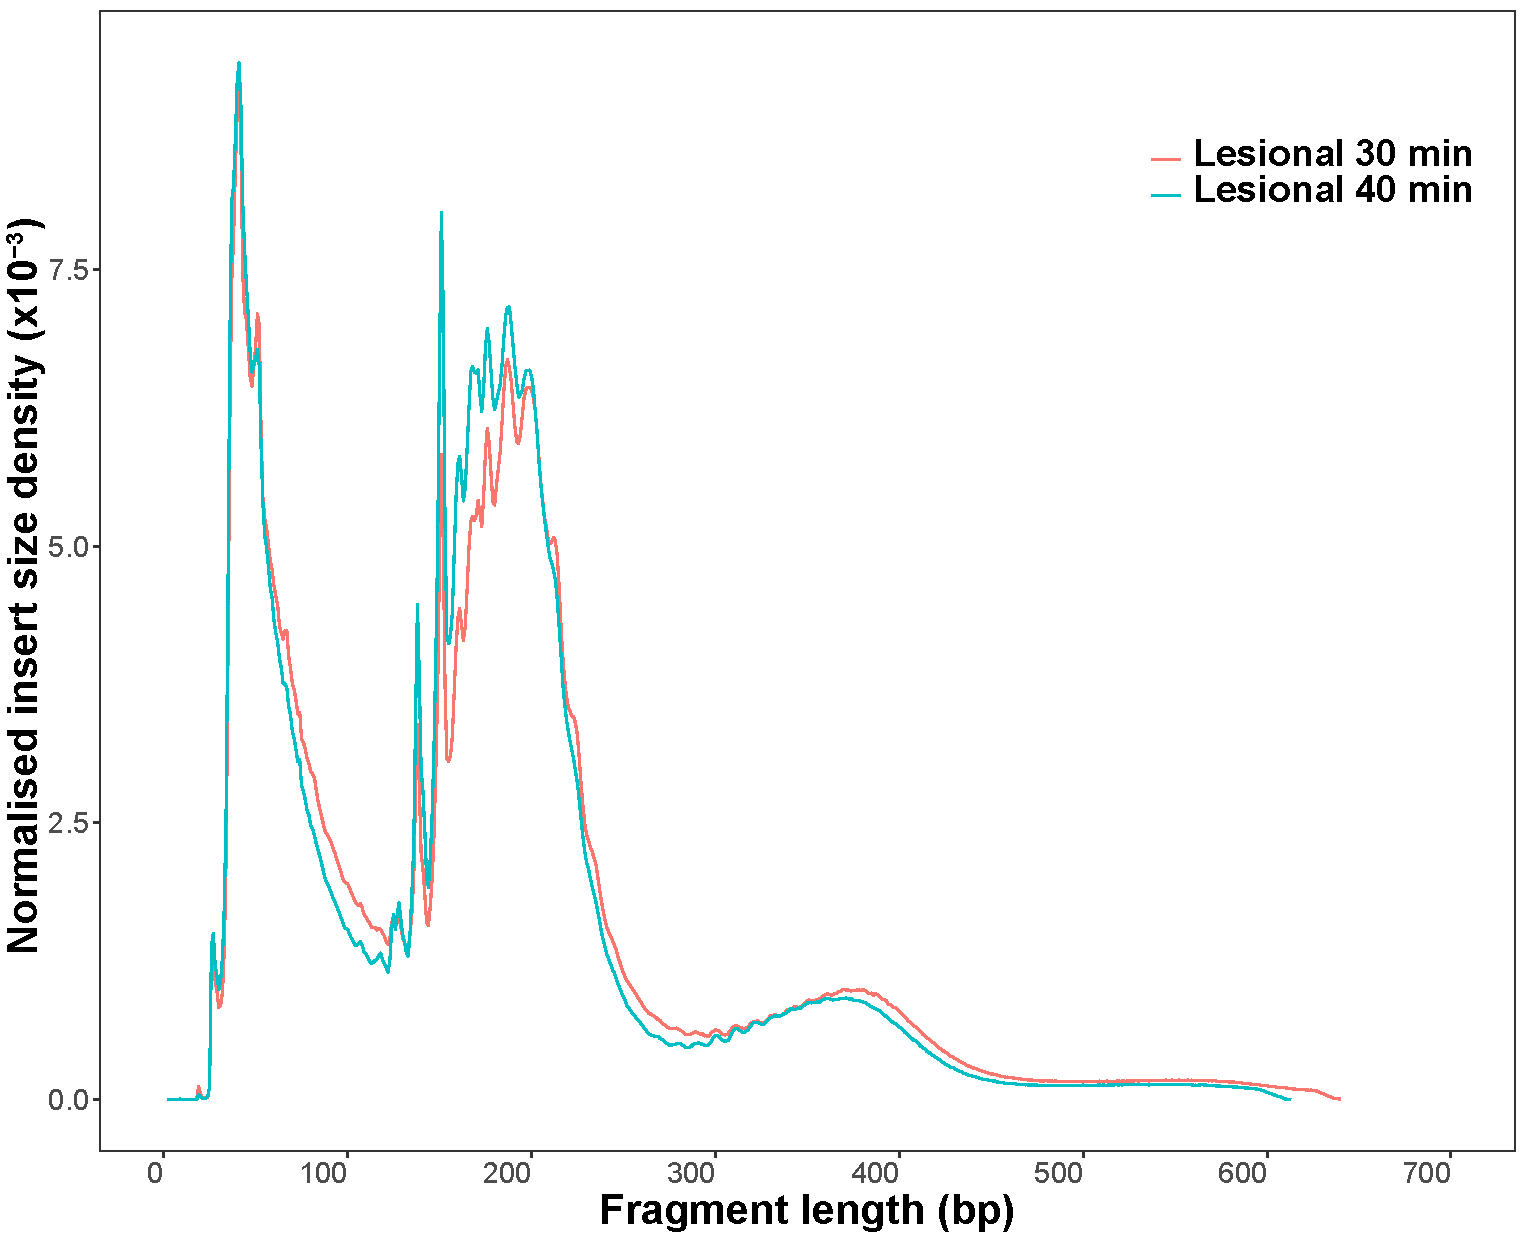
\includegraphics[width=\textwidth]{./Results1/pdfs/ATAC_PS-2_30_40_min_fragment_size_distribution}
\caption{\textbf{}}
\end{subfigure}%
\begin{subfigure}{0.45\textwidth}
\centering
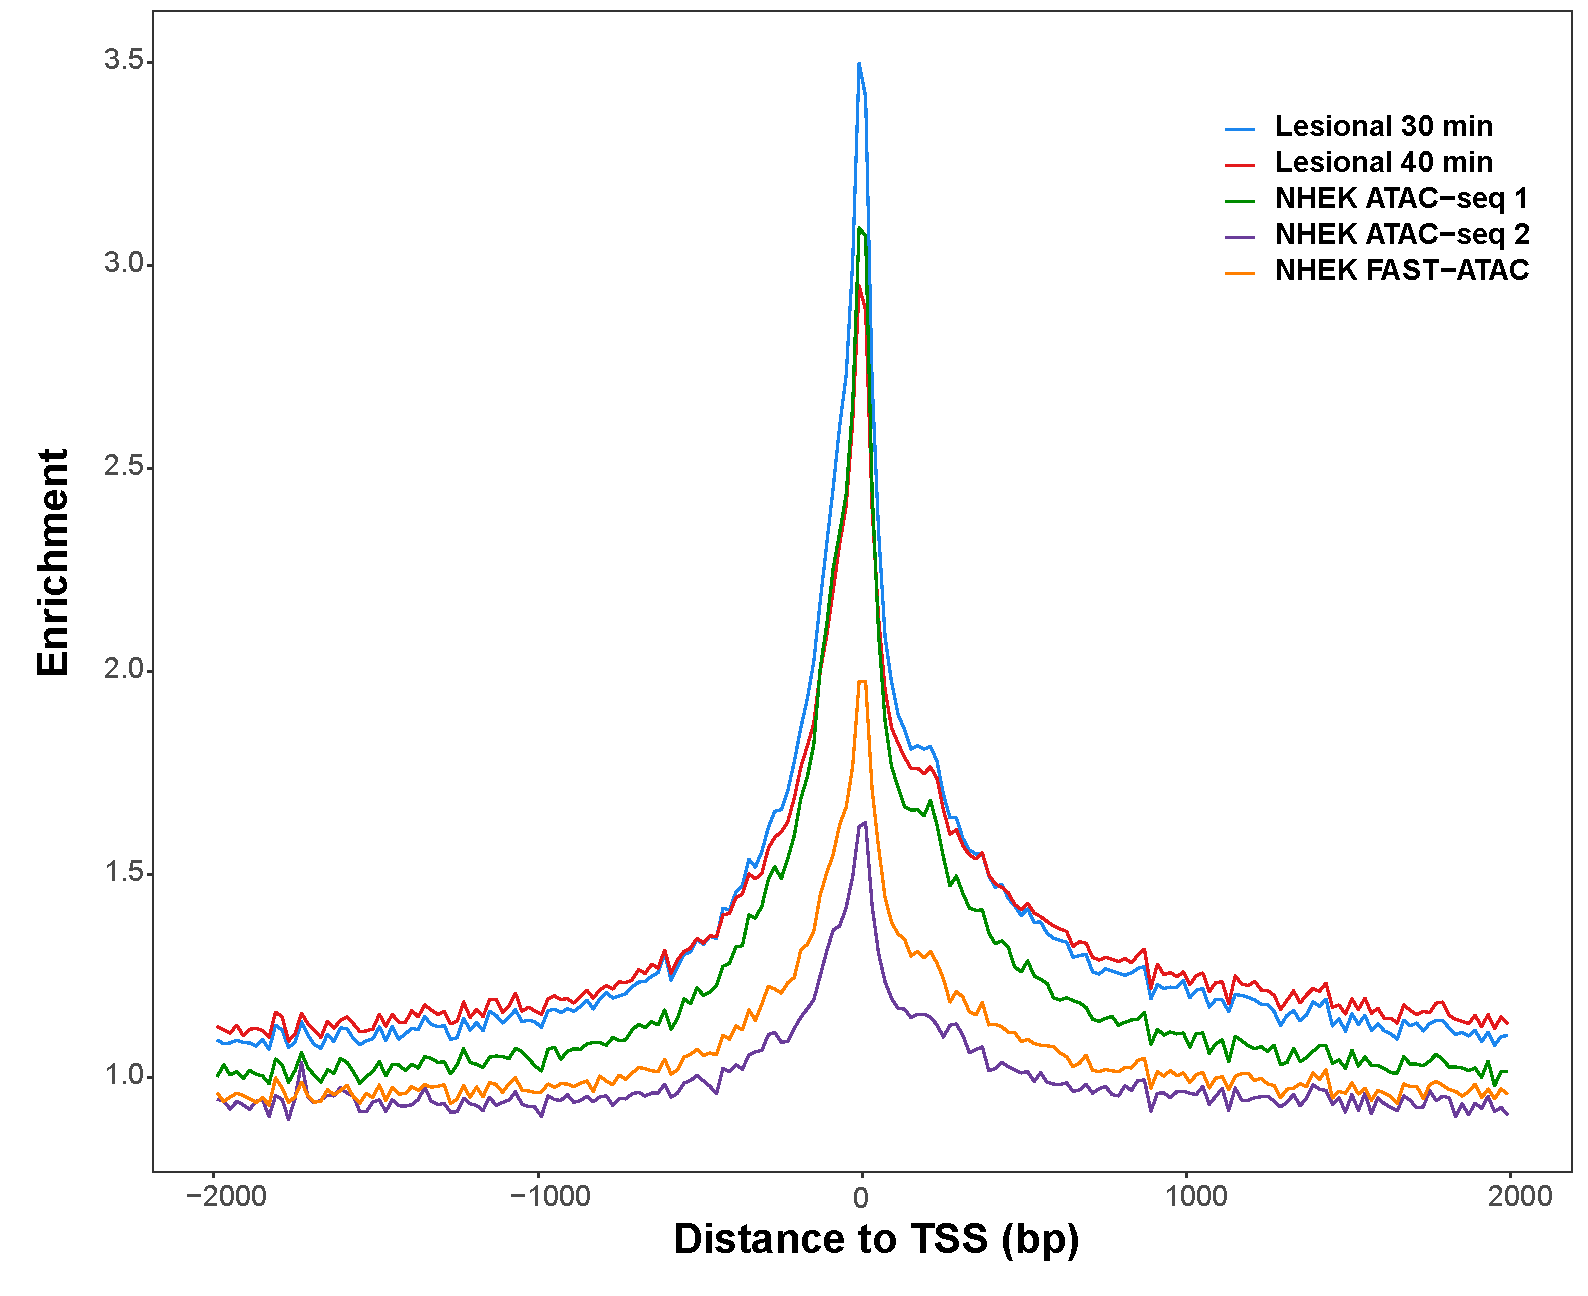
\includegraphics[width=\textwidth]{./Results1/pdfs/ATAC_skin_TSS_enrichment_PS02_30_40min_NHEK_ATAC1_ATAC_2_FAST_ATAC}
\caption{\textbf{}} % to add text to the figure name
\end{subfigure}
\caption[Quality control assessment of different ATAC protocols in keratinocytes from a psoriatic lesion and NHEKs.]{\textbf{Quality control assessment of different ATAC protocols in keratinocytes from a psoriatic lesion and NHEKs.} (A) Pre-sequencing quantification of DNA fragment sizes in the ATAC libraries and (B) the density distribution of sequenced fragments for ATAC 1 libraries generated in 50,000 keratinocytes in suspension isolated from lesional skin from a psoriasis patient. Two transposition times (30 and 40 min) were tested in the same sample keratinocytes suspension and only the pre-sequencing profiles of relative abundance of DNA library fragment sizes at 30 min transposition has been included. The pre-sequencing profiles of relative abundance of DNA library fragment sizes for 40 min transposition is in Figure \ref{figure:PS2_40min_tapestation}. (C) Fold-enrichment of ATAC fragments across the Ensembl annotated TSS from the ATAC 1 psoriasis lesional keratinocytes libraries (previously mentioned in (A) and (B) and NHEK libraries generated with ATAC 1, ATAC 2 and Fast-ATAC protocols performed directly on the 96-well plate adherent cells.}
\label{figure:PS02_skin_ATAC_QC_assessment}
\end{figure} 


Following Buenrostro and colleagues' ATAC-seq protocol, a modified version for keratinocytes by Bao and colleagues (named ATAC 2 in this subsection) and the Fast-ATAC protocols were released \parencite{Bao2015, Corces2016}. Interestingly, Bao's protocol was applied directly on the cell culture plate containing adherent NHEKs, avoiding a trypsinisation step that could increase cell death. In line with Baoand colleagues protocol, to prevent background noise due to presence of dead cells affecting the assessment of the different protocols, two systems were implemented. First, all the cells obtained from the epidermis of control skin biopsies were cultured for 3h in a 96-well plate and washed afterward to minimise the presence of apoptotic cells. This procedure, known as adherence assay, allows the isolation of viable undifferentiated keratinocytes. Second, cultured NHEKs (50,000 cells) were also incorporated as a control to test the performance of the different ATAC protocols. The three ATAC protocols (ATAC 1, ATAC 2 and Fast-ATAC using C1 conditions, Table \ref{tab:ATAC_skin_optimisation_protocols}) were performed directly on the plate adherent cells with no cell detachment step. 



\begin{table}[htbp]
%\setlength{\tabcolsep}{20pt}
%\renewcommand{\arraystretch}{1.5}
\begin{tabular}{@{} c c c}
\toprule
\textbf{Protocol}   & \textbf{Lysis and} & \textbf{Key parameters} \\
                    & \textbf{transposition} &  \\
\midrule
\midrule
ATAC 1          & Two steps & 0.1\% NP-40 and 2.5$\micro$L Tn5  \\
\parencite{Buenrostro2013} && \\
&&\\
ATAC 2          &Two steps   & 0.05\% NP-40 and 5$\micro$L Tn5  \\
\parencite{Bao2015} &&\\
&&\\
                                 &             & C1$^\ast$: 0.01\% digitonin, 2.5$\micro$L Tn5 \\
 Fast-ATAC                       &             & C2: 0.01\% digitonin, 0.5$\micro$L Tn5 \\
\parencite{Corces2016}           & One step    & C3: 0.025\% digitonin, 0.5$\micro$L Tn5 \\
													       &             & C4: 0.025\% digitonin, 2.5 $\micro$L Tn5 \\
\bottomrule
\end{tabular}
\medskip %gap
\caption[Description of the most relevant parameter from the ATAC-seq and FAST-ATAC protocols assayed in NHEK and skin biopsies.]{\textbf{Description of the most relevant parameter from the ATAC-seq and FAST-ATAC protocols assayed in NHEK and skin biopsies.}Transposition times for all protocols was 30 min. $^\ast$ corresponds to the original Fast-ATAC conditions from Corces \textit{et al.}, 2016.}
\label{tab:ATAC_skin_optimisation_protocols}
\end{table}
\bigskip %bigger space

For all three protocols, the library size distribution of sequenced fragments showed the presence of NFR and a poorly defined nucleosome pattern, particularly for the ATAC 2 protocol in both NHEKs and adherent keratinocytes from skin biopsies (Figure \ref{figure:ATAC_skin_optimisation_protocols}A). Similarly to the results in cell suspensions from psoriatic lesional epidermis, TSS enrichments were very low, particularly for the ATAC 2 protocol, and in all the instances under the acceptable cut-off using the two cell systems (Figures \ref{figure:PS02_skin_ATAC_QC_assessment}C and \ref{figure:TSS_skin_biopsies}).

Further optimisation of the Fast-ATAC protocol was performed by modifying the original concentration of NP-40 detergent and the Tn5 enzyme (Table \ref{tab:ATAC_skin_optimisation_protocols} C1-4). Library quality control using pre-sequencing profiles of relative abundance of DNA library fragment sizes to assess the DNA fragment size distributions failed to show the nucleosome pattern profile expected in ATAC, and therefore the samples did not proceed to NGS (Figure \ref{figure:NHEK_tapestation}A, B and C).

 

\begin{figure}[htbp]
\centering
\begin{subfigure}{0.48\textwidth}
\centering
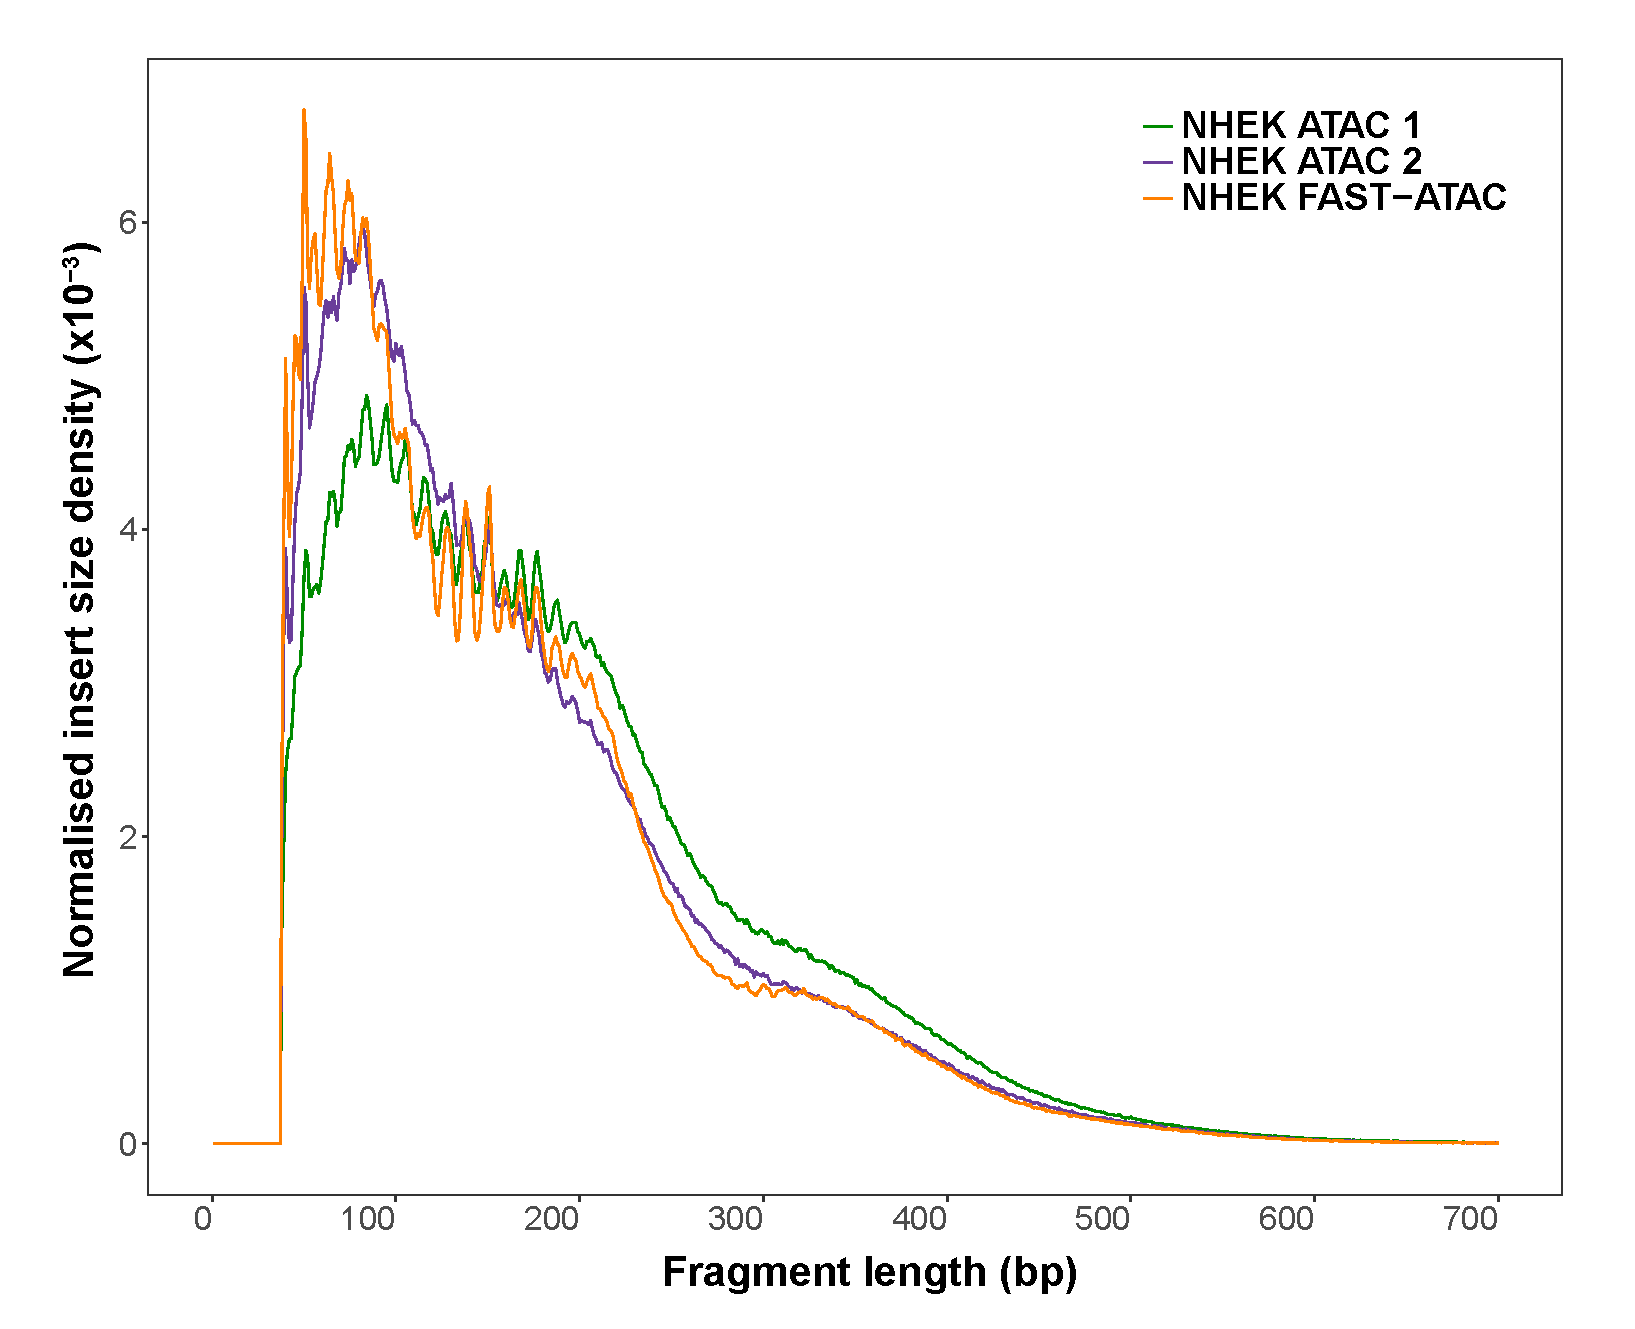
\includegraphics[width=\textwidth]{./Results1/pdfs/ATAC_NHEK_ATAC1_ATAC2_FAST_ATAC_fragment_size_distribution}
\caption{\textbf{}}
\end{subfigure}%
\begin{subfigure}{0.48\textwidth}
\centering
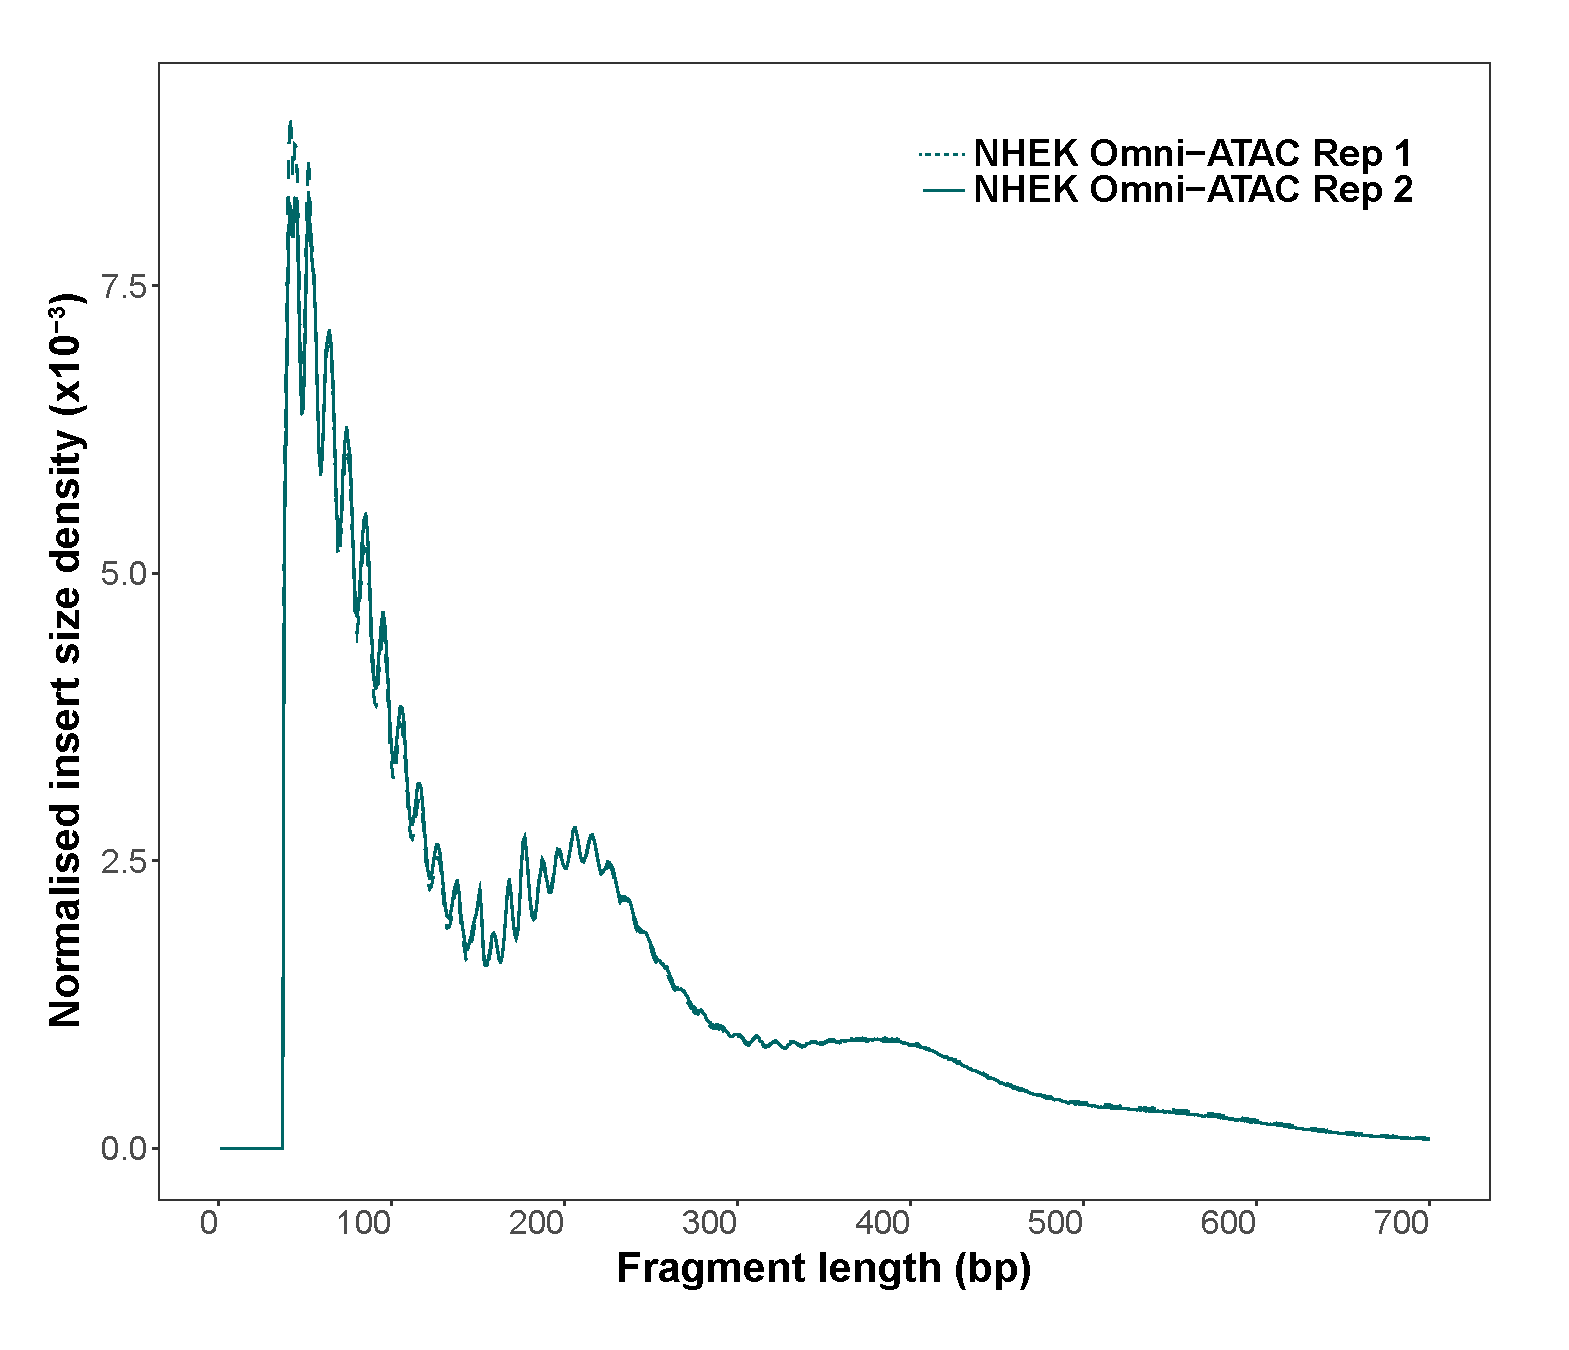
\includegraphics[width=\textwidth]{./Results1/pdfs/ATAC_NHEK_Omni_ATAC_fragment_size_distribution}
\caption{\textbf{}}
\end{subfigure}
\begin{subfigure}{0.5\textwidth}
\centering
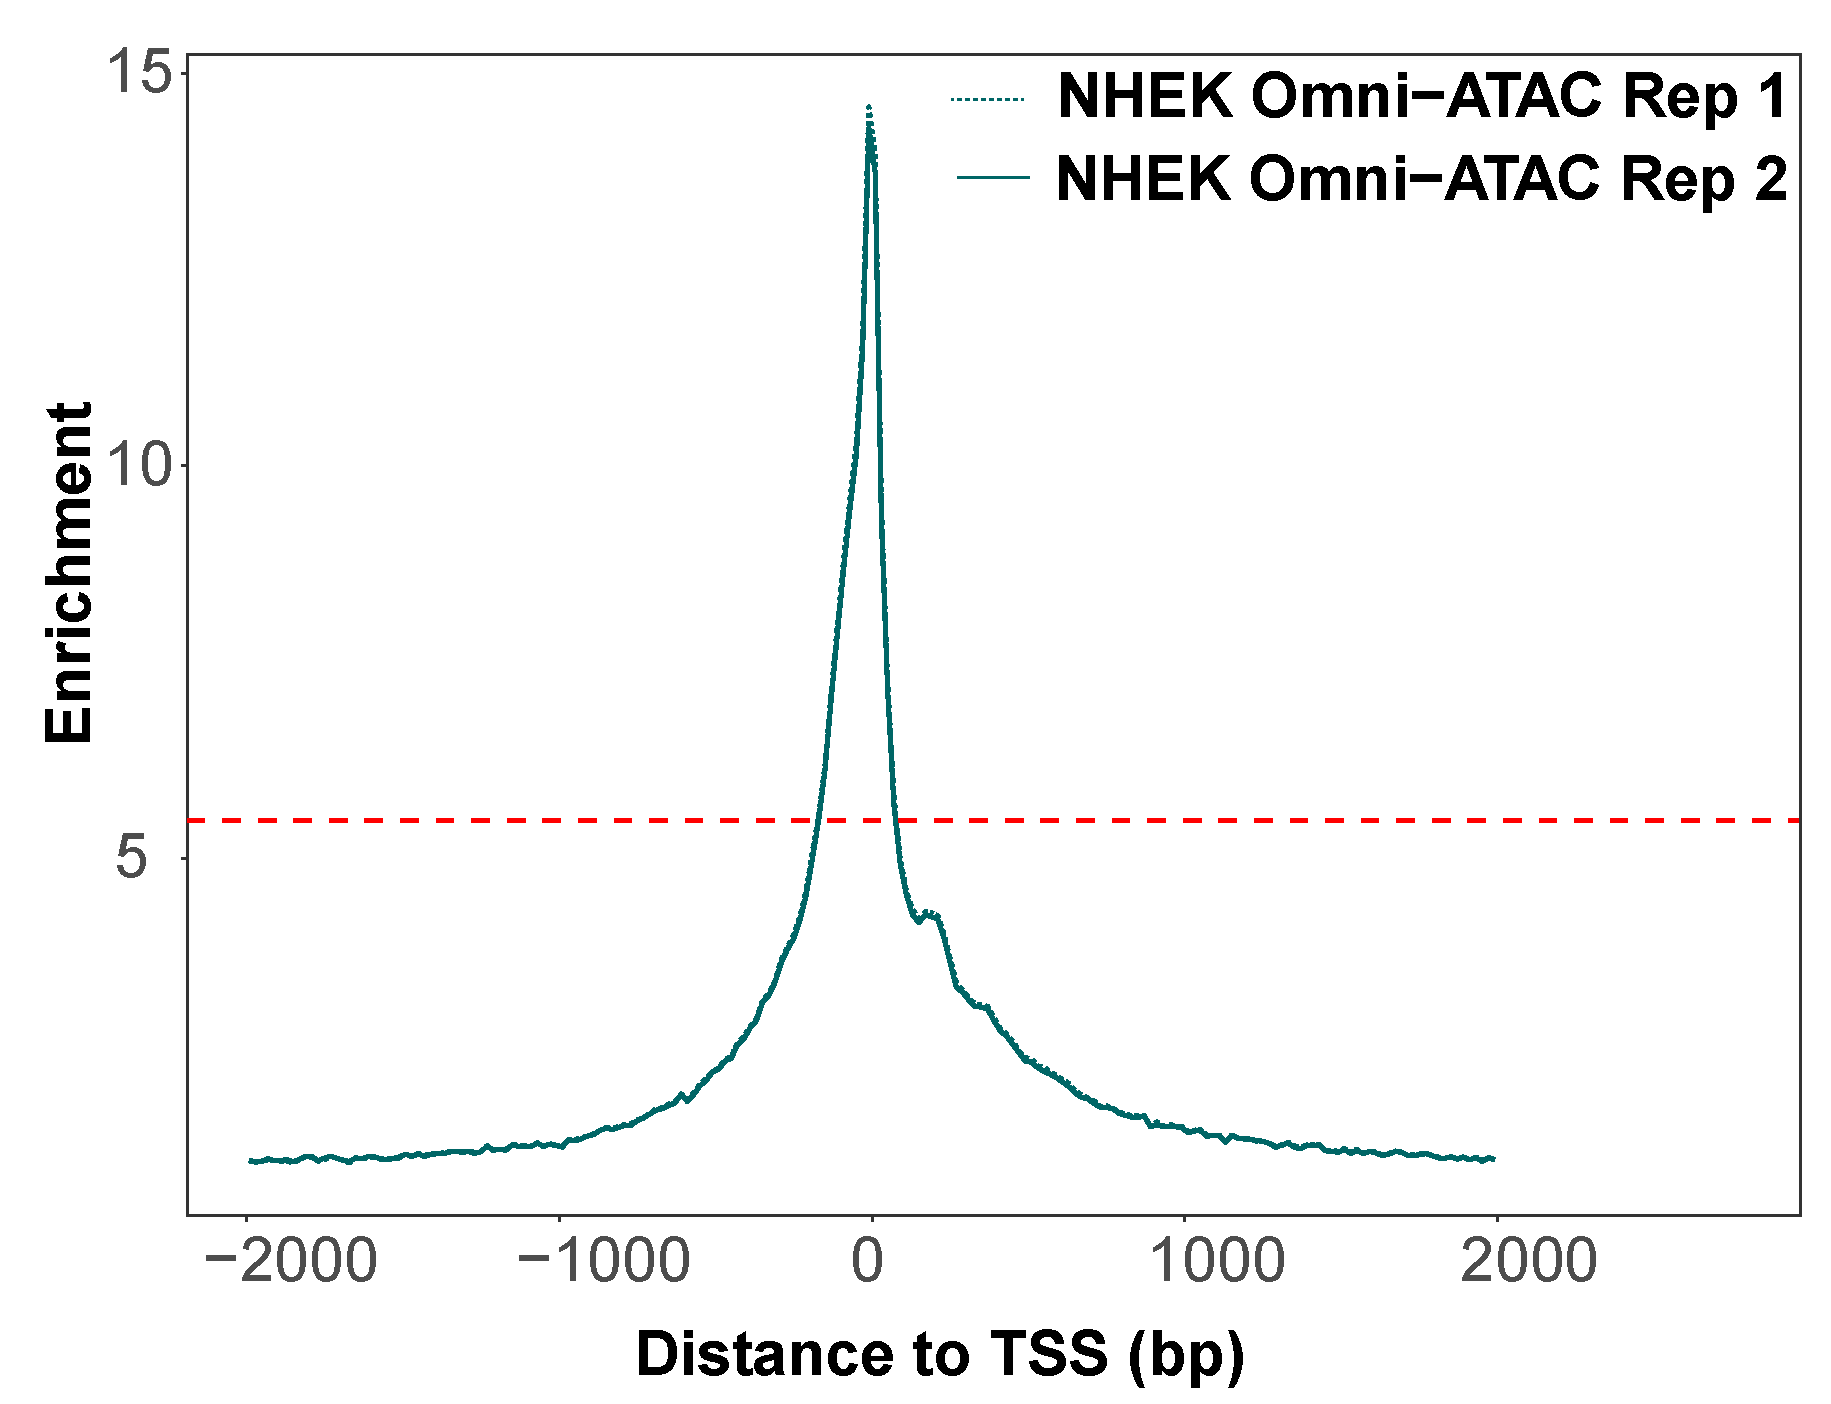
\includegraphics[width=\textwidth]{./Results1/pdfs/ATAC_skin_TSS_enrichment_NHEK_omni_ATAC}
\caption{\textbf{}} % to add text to the figure name
\end{subfigure}%
\caption[Quality control assessment of Fast-ATAC and Omni-ATAC in cultured NHEK]{\textbf{Quality control assessment of Fast-ATAC and Omni-ATAC in cultured NHEK.} Representation of the fragment sizes density distribution in NHEKs libraries generated using (A)ATAC1, ATAC2 and Fast-ATAC or (B) Omni-ATAC protocols. (C) Fold-enrichment of ATAC fragments across the Ensembl annotated TSS from two Omni-ATAC technical replicates.}
\label{figure:PS02_skin_ATAC_QC_assessment}
\end{figure} 


Towards the end of experimental work for this thesis, a new protocol called Omni-ATAC was published \parencite{Corces2017}. Omni-ATAC was a protocol suitable for every cell type, in contrast to ATAC 1 and Fast-ATAC, which were optimised for hematopoietic cells \parencite{Buenrostro2013,Corces2016}. Performance of this protocol in 50,000 viable NHEKs in suspension yielded the expected fragment size distribution for sequenced fragments, with the greatest abundance for NFR followed by mono and di-nucleosome fragments (Figure \ref{figure:PS02_skin_ATAC_QC_assessment}B). Moreover, high TSS enrichment values (approximately 20 fold) were observed for the two replicates (Figure \ref{figure:PS02_skin_ATAC_QC_assessment} c). When performing overlap between the Omni-ATAC sample peaks filtered for a low stringency p-value (p-value=0.01) and the ENCODE DHSs from 125 cell types, the highest percentage (approximately 55\%) was reported for NHEKs (Figure \ref{figure:ATAC_skin_ENCODE_overlap_and_tracks}A).

\begin{figure}[htbp]
\centering
\begin{subfigure}{0.5\textwidth}
\centering
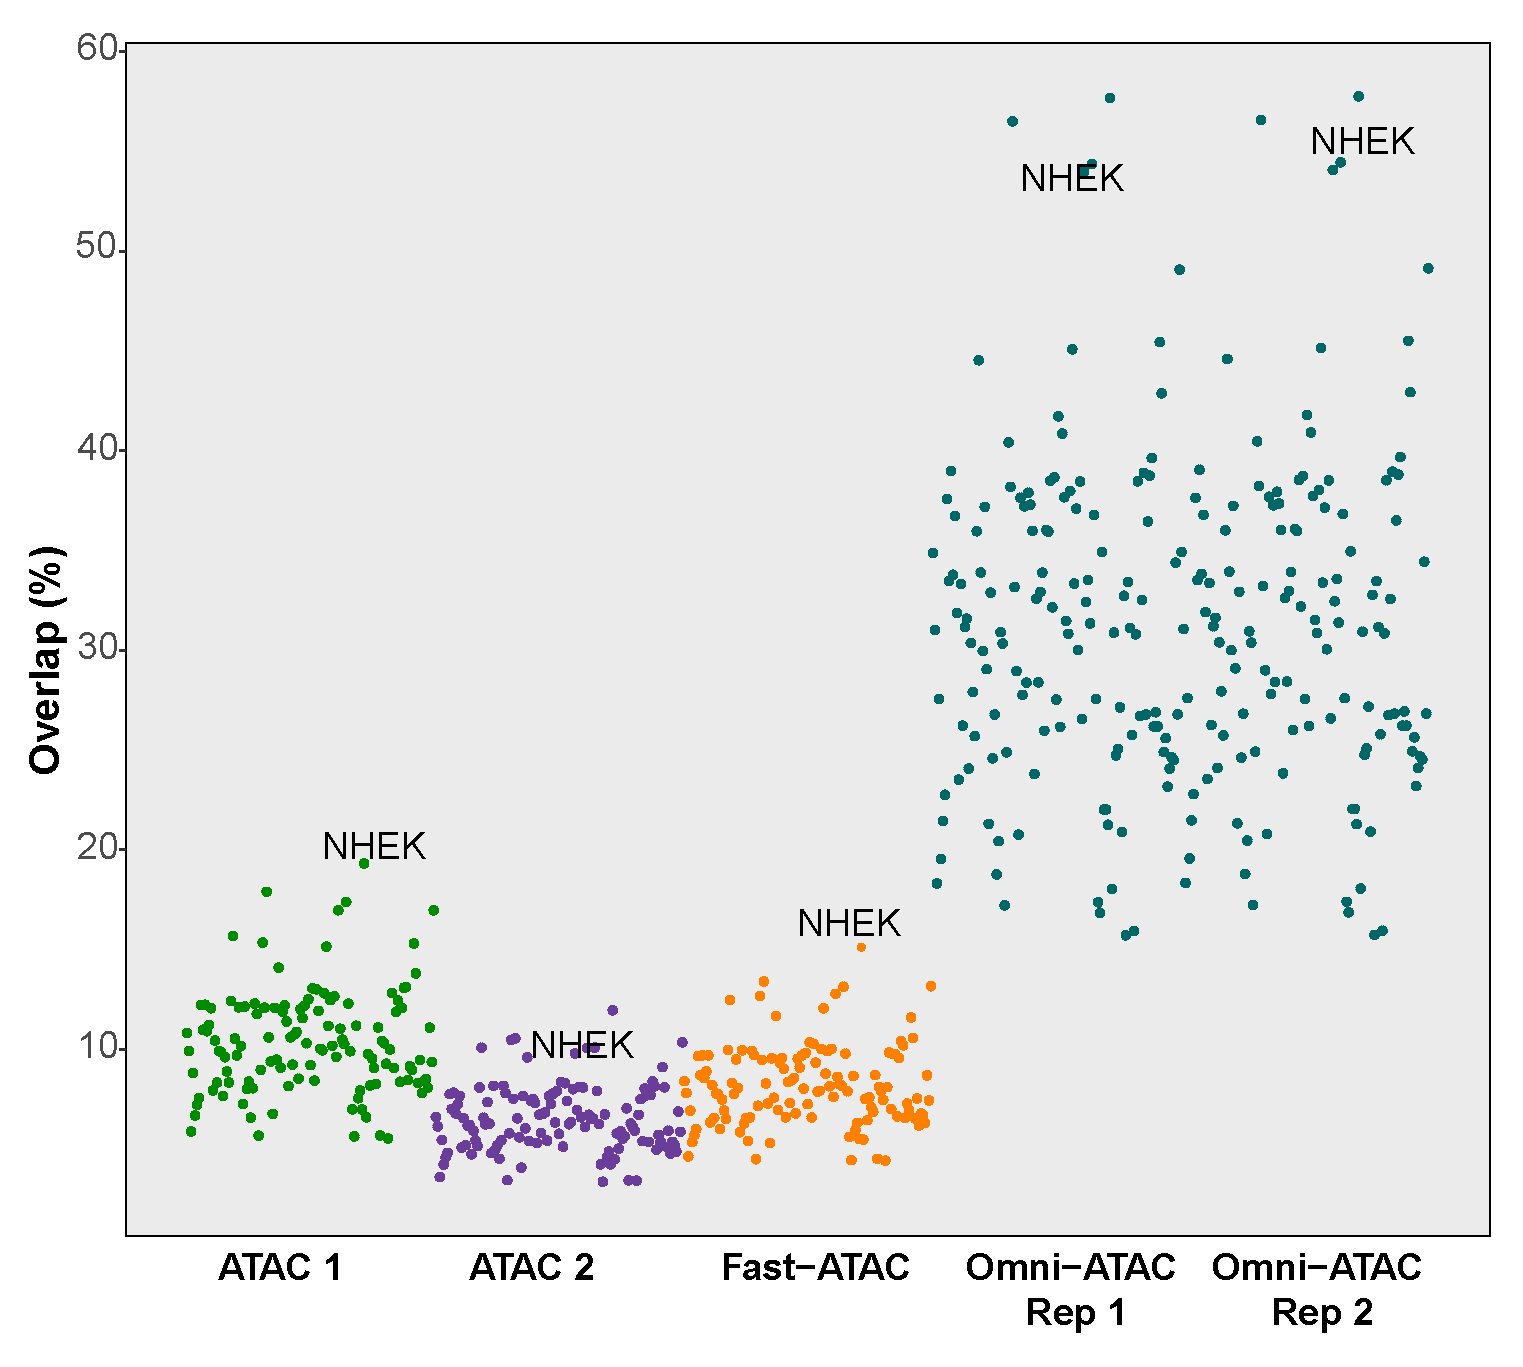
\includegraphics[width=\textwidth]{./Results1/pdfs/ENCODE_125_cell_types_overlap_FAST_ATAC_Omni_ATAC_pval_2}
\caption{\textbf{}}
% The percentage sign indicated that the other subfig goes side by side
\end{subfigure}
\begin{subfigure}{0.5\textwidth}
\centering
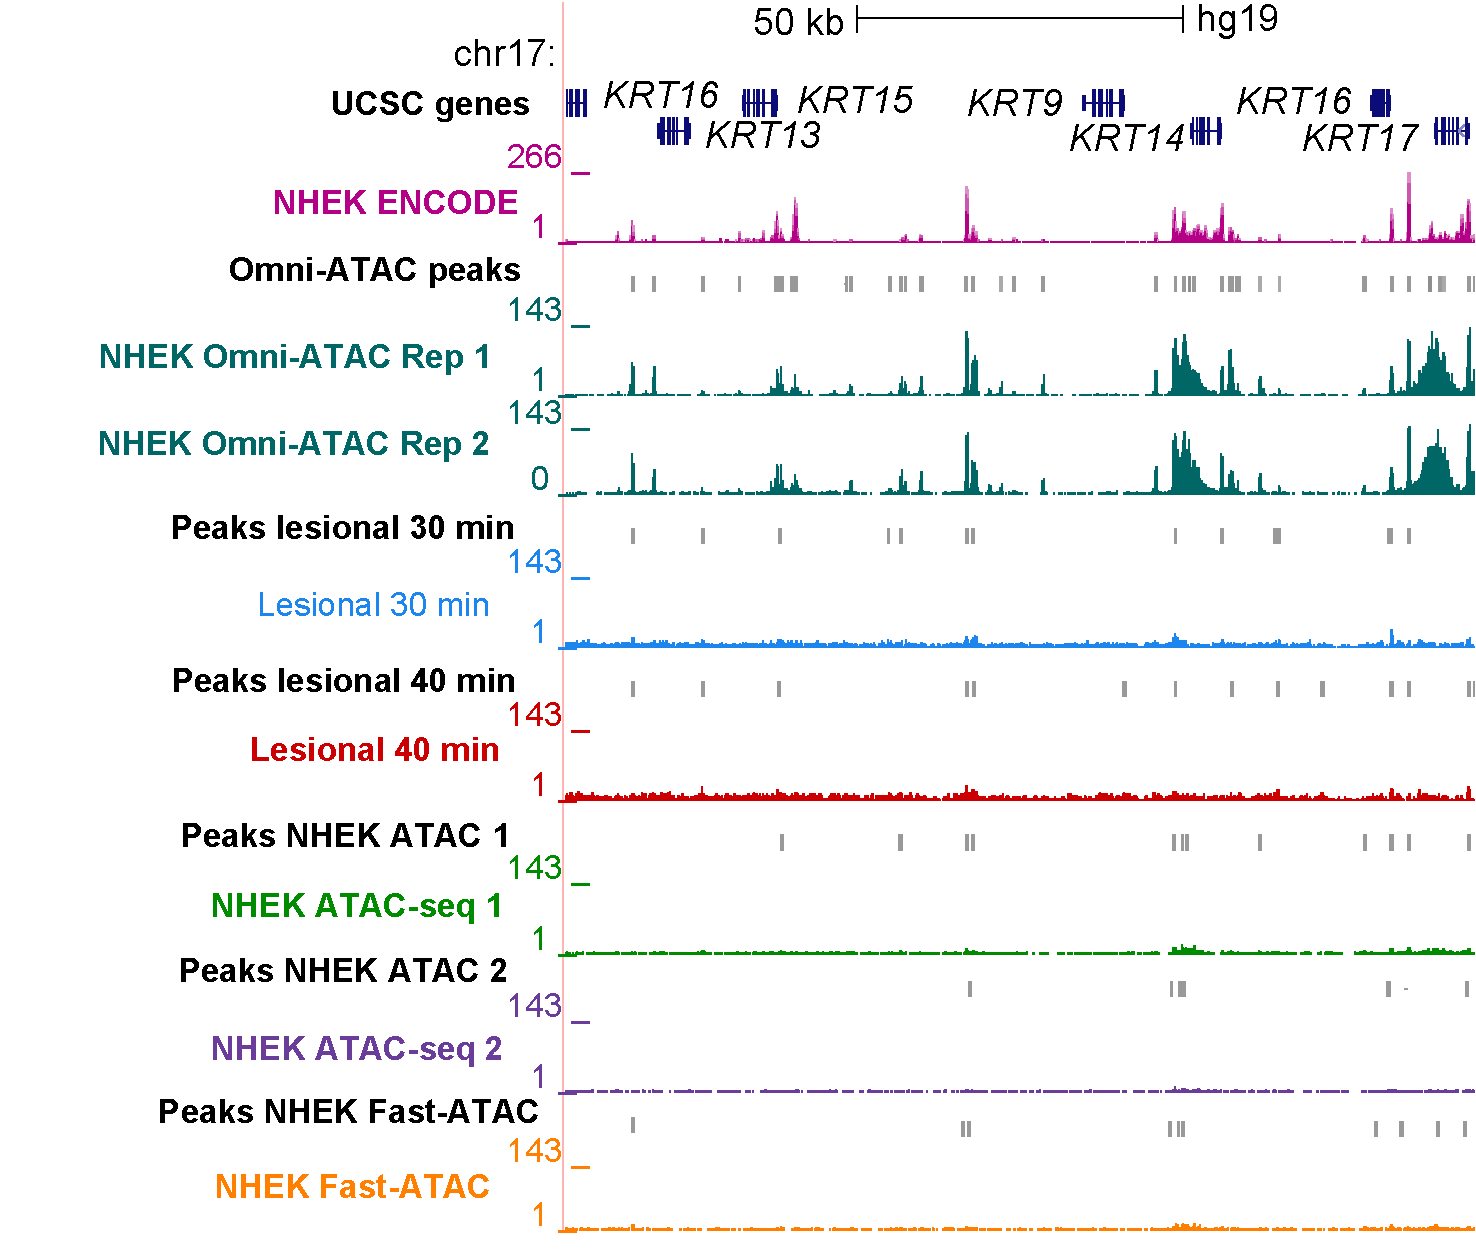
\includegraphics[width=\textwidth]{./Results1/pdfs/ATAC_skin_all_tracks_KRT}
\caption{\textbf{}}
\end{subfigure}
\caption[Comparison of 4 different ATAC protocols applied to psoriasis and/or healthy keratinocytes and NHEKs cells with published ENCODE DNase-seq data.]{\textbf{Comparison of 4 different ATAC protocols applied to psoriasis and/or healthy keratinocytes and NHEKs cells with published ENCODE DNase-seq data.} (A) Enrichment (\% of overlap) of observed peaks called in each ATAC sample (using low stringent p-value) with open DHS chromatin regions in 125 ENCODE cell types. (B) UCSC Genome Browser track showing open chromatin at the chr17 keratin (KRT) family gene locus for different ATAC protocols with the normalised ATAC read density (y-axis) shown.}
\label{figure:ATAC_skin_ENCODE_overlap_and_tracks}
\end{figure} 

In contrast, the same analysis for the ATAC 1, ATAC 2 and Fast-ATAC peaks only showed 20\% or less overlap with ENCODE NHEKs, supporting the higher quality and specificity of Omni-ATAC accessible regions in keratinocytes, even at a very low p-value filtering. The differences in the quality of ATAC signal between Omni-ATAC and the prior ATAC protocols was clearly observed at the chr17 locus harbouring a number of keratin genes, which encode the main components of keratinocyte cytoskeleton (Figure \ref{figure:ATAC_skin_ENCODE_overlap_and_tracks}B). Omni-ATAC clearly showed the lowest background noise, the highest signal intensity and the greatest number of high quality peaks across the different keratin (KRT) genes when compared to the samples generated with the other ATAC protocols. %Overall, this data was consistent with Corces \textit{et al.}, 2017, where consistent successful results in NHEKs were shown, and it encourages future testing of Omni-ATAC in keratinocytes from psoriasis patients biopsies processed through adherent assay to minimise the presence of dead cells.


\subsection{Effect of cryopreservation and fixation in the chromatin landscape of immune primary cells}
\label{Core}
\subsubsection{Experimental design and sample description}
As previously introduced, research using clinical samples represents a logistical challenge as immediate processing of freshly acquired cells may not be feasible. In the context of this thesis, two different possible approaches involving cryopreservation and fixation were of interest and a collaborative project to investigate these was established with High-Throughput Genomics at the WHG. The first approach was the cryopreservation of PBMCs in liquid nitrogen using DMSO followed by thawing, recovery and FACS isolation of the cell population of interest (Figure \ref{figure:Core_experimental_design}). Secondly, the performance of an optimised protocol developed by High-Throughput Genomics using DSP in scRNA-seq \parencite{Attar2018} was investigated as a short term preservation method for FACS-isolated relevant cell types.

In order to investigate the performance of these two strategies, blood from 3 healthy volunteers (Chapter \ref{ch:Results1} in \ref{tab:Summary_all_cohorts}) matched for sex and age (3 females, mean age 25.6 years old) was processed on different days to simulate the experimental design when using patient samples (experimental design summarised in Figure \ref{figure:Core_experimental_design}). PBMCs were prepared from 90mL blood using a Ficoll gradient and CD14$^+$ monocytes and CD4$^+$ T cells were isolated by FACS, as detailed in Chapter \ref{ch:Mat}. ATAC-seq was performed on 50,000 CD14$^+$ mpnocytes and CD4$^+$ T cells, either freshly isolated or after fixation with DPS, stored at 4{$^\circ$}C for 24h and then processed for ATAC-seq (Figure \ref{figure:Core_experimental_design} Day 1, ATAC-seq fres and ATAC-seq fixed, respectively). To investigate the utility of cryopreservation, 70x10$^6$ million PBMCs were cryopreserved on the day of collection and stored in liquid nitrogen followed by thawing and recovery in culture for approximately 30 min (as detailed in Chapter \ref{ch:Mat}). After recovery, CD14$^+$ monocytes and CD4$^+$ T cells were isolated from the PBMCs by FACS and then ATAC-seq was performed (Figure \ref{figure:Core_experimental_design} Day 7, ATAC-seq frozen). Altogether, for each volunteer, 3 matched ATAC-seq libraries were generated in two different cell populations: ATAC-seq fresh, ATAC-seq fixed and ATAC-seq frozen.

\begin{landscape}
\begin{figure}[H]
\centering
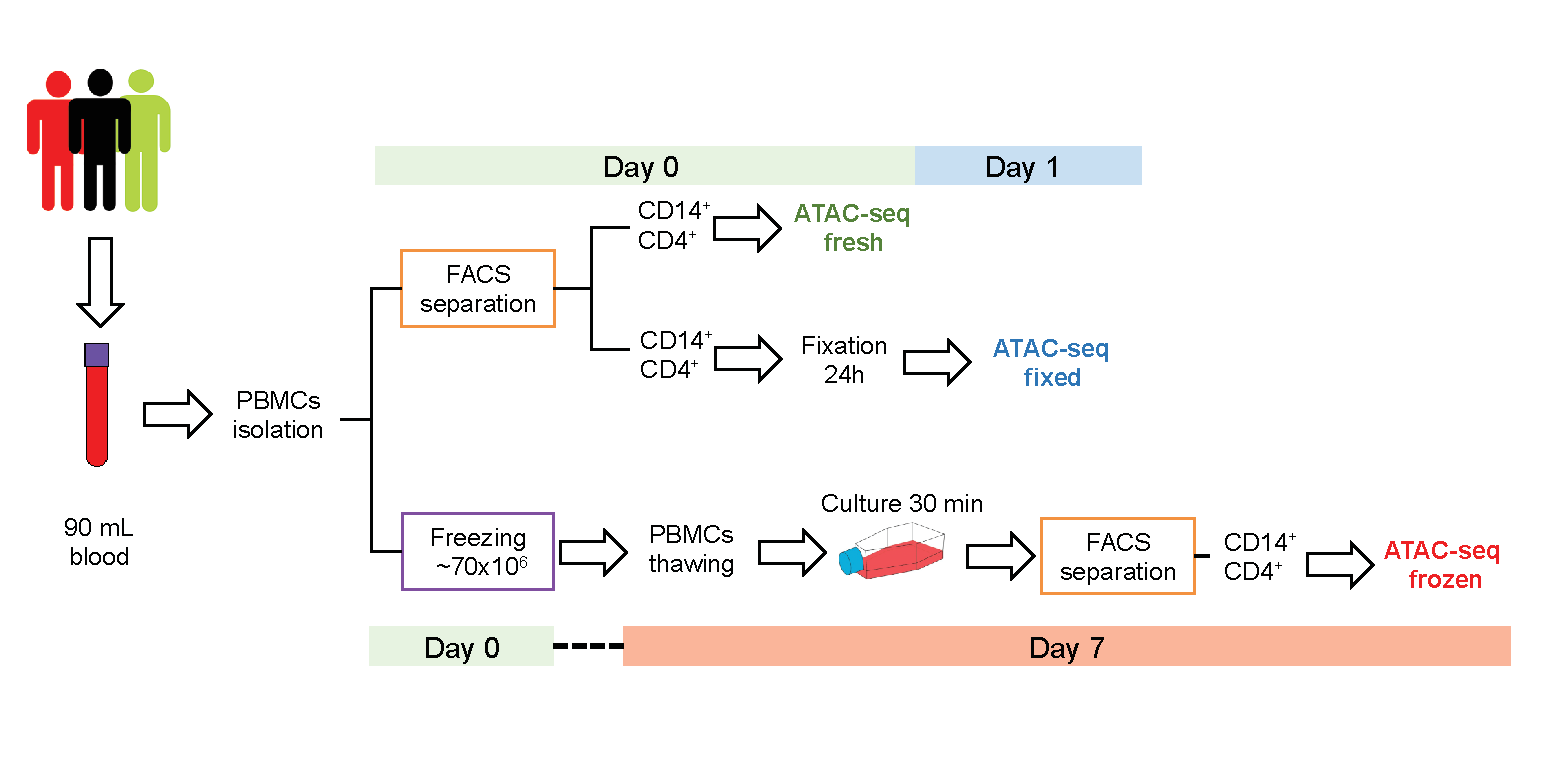
\includegraphics[width=1.2\textwidth]{./Results1/pdfs/Chapter3_core_experimental_design}
\caption[Experimental design to assess the impact of cryopreservation and fixation in the chromatin accessibility of immune primary cells.]{\textbf{Experimental design to assess the impact of cryopreservation and fixation in the chromatin accessibility of immune primary cells.} Three healthy control individuals were recruited on different days, PBMCs were isolated and freshly isolated CD14$^+$ monocytes or CD4$^+$ T cells processed for ATAC-seq immediately (ATAC-seq fresh), after fixation with DPS (ATAC-seq fixed) or after cryopreservation of PBMCs (ATAC-seq frozen).%Three healthy control individuals were recruited on different days and PBMCs were isolated from 90mL of blood (Day 0). on Day 0, a fraction of PBMCs were used for FACS staining and isolation of 50,000 CD14$^+$ and CD4$^+$, which were directly processed for ATAC-seq (ATAC-seq fresh). Also on Day 0, a 50,000 FACS-sorted CD14$^+$ and CD4$^+$ cells were fixed with DPS, stored at 4{$^\circ$}C for 24h and processed for ATAC-seq in Day 1 (ATAC-seq fixed). Lastly, on Day 0 a fraction of the PBMCs (70x10$^6$ million cells) were cryopreserved in DMSO and slow-cooling. On Day 7 of storage in liquid nitrogen, PBMCs were thawed, recovered in culture for 30 min and stained with FACS Abs to isolate 50,000 CD14$^+$ and CD4$^+$cell to perform ATAC-seq (ATAC-seq frozen).}
\label{figure:Core_experimental_design}
\end{figure}
\end{landscape}



\subsubsection{Chromatin accessibility in the different experimental conditions}

All samples from each of the two cell types had more than 15 million reads, which have previously been shown as the minimum for successful ATAC-seq analysis and peak calling (Figure \ref{figure:Core_ATAC_all_conditions_total_reads}). The median number of reads across the fresh, frozen and fixed were more similar for CD14$^+$ monocytes (58.6, 64.2 and 39.6 million reads, respectively) than in the CD4$^+$ samples, where the frozen and fixed presented lower median total reads compared to the controls (43.8, 32.9 and 28.8 million reads respectively)(Figure \ref{figure:Core_ATAC_all_conditions_total_reads}A and B).

\begin{figure}[htbp]
\centering
\begin{subfigure}{0.5\textwidth}
\centering
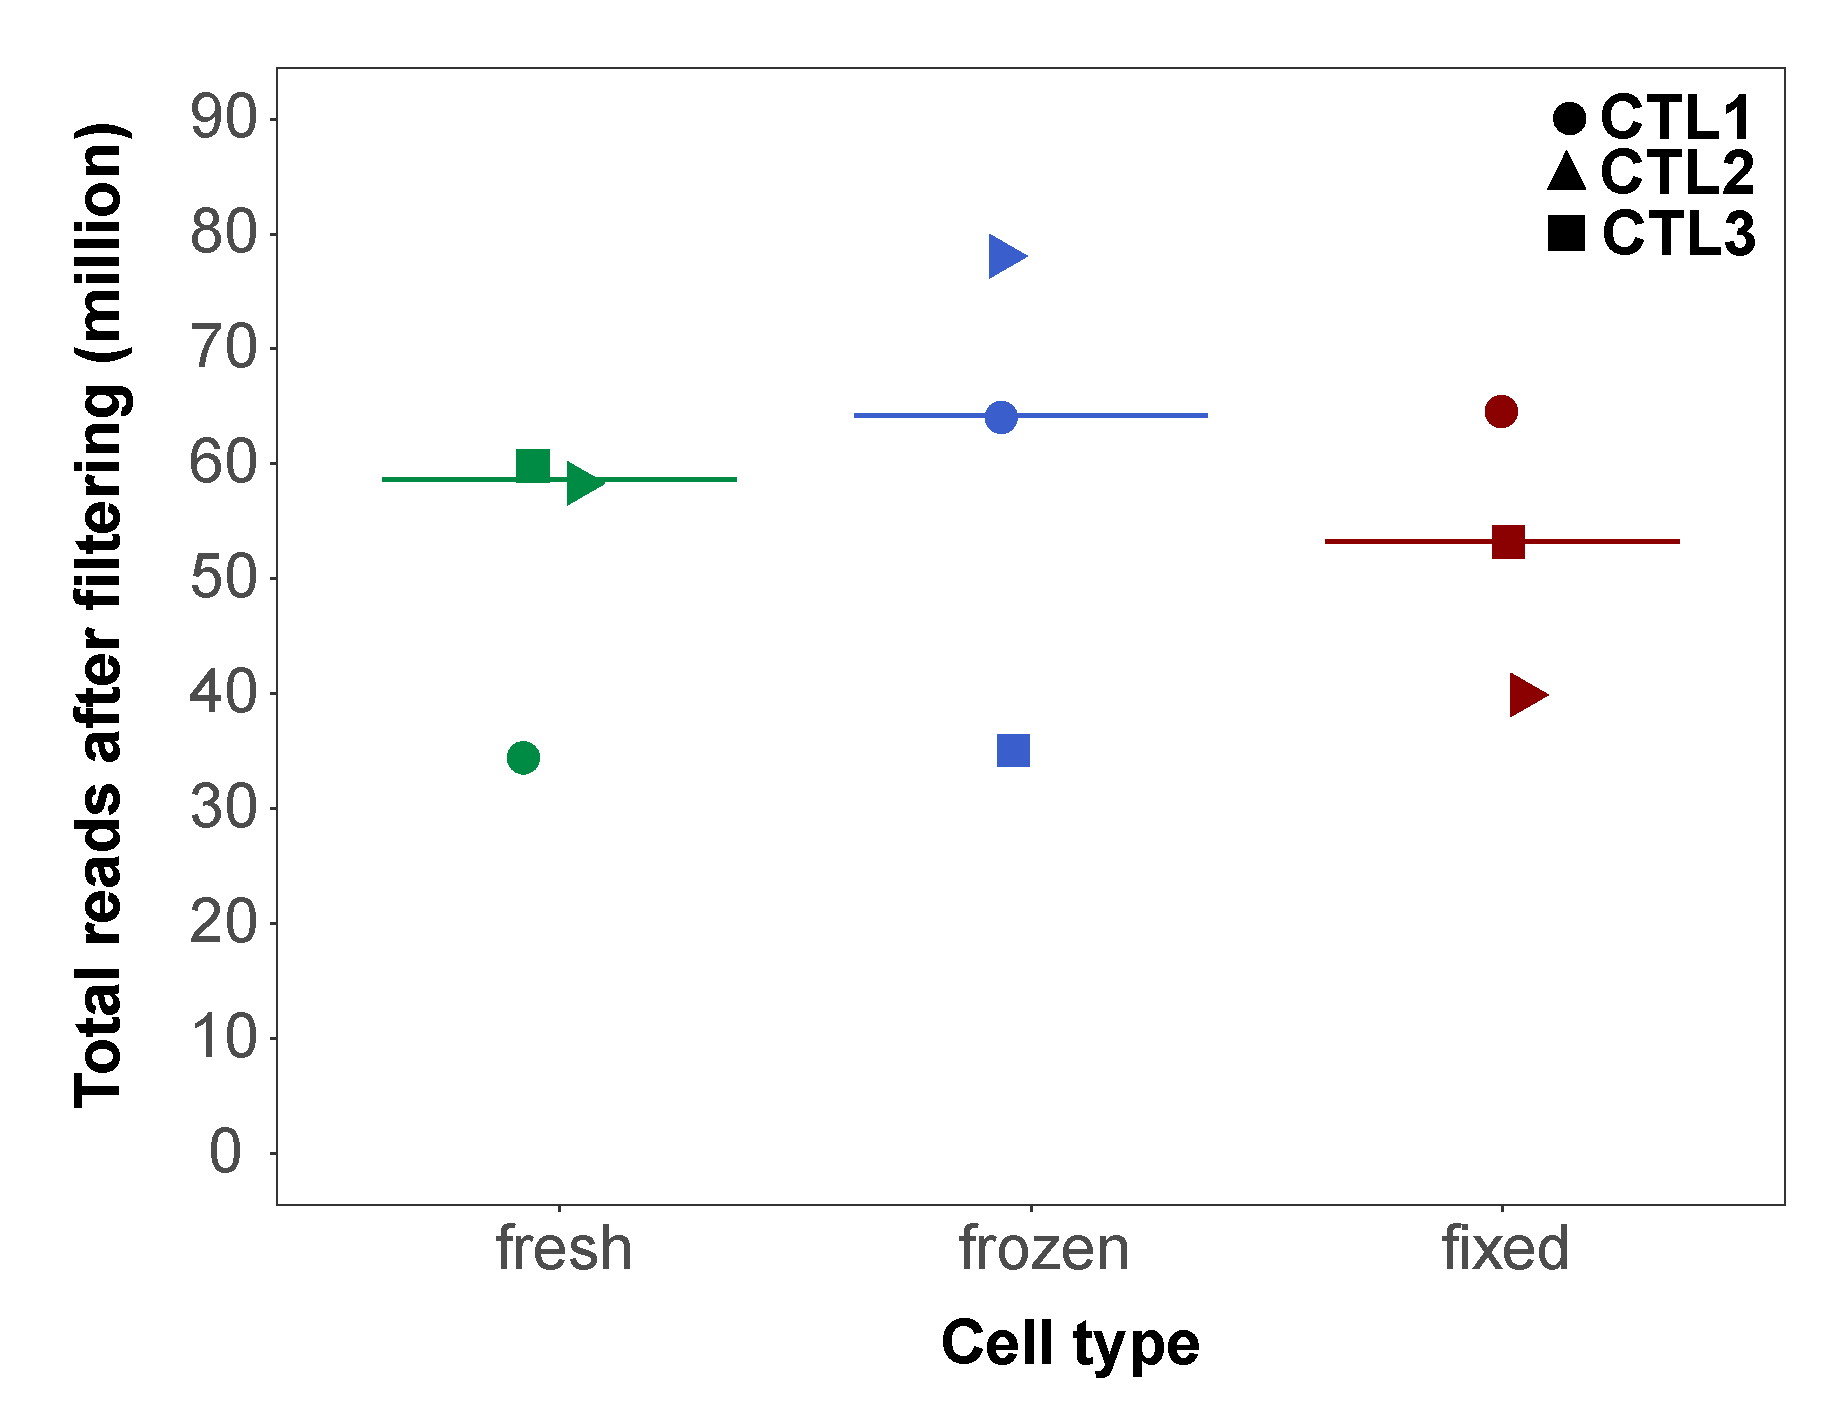
\includegraphics[width=\textwidth]{./Results1/pdfs/Core_ATAC_CD14_fresh_frozen_fixed_filtered_total_reads}
\caption{\textbf{}}
% The percentage sign indicated that the other subfig goes side by side
\end{subfigure}%
\begin{subfigure}{0.5\textwidth}
\centering
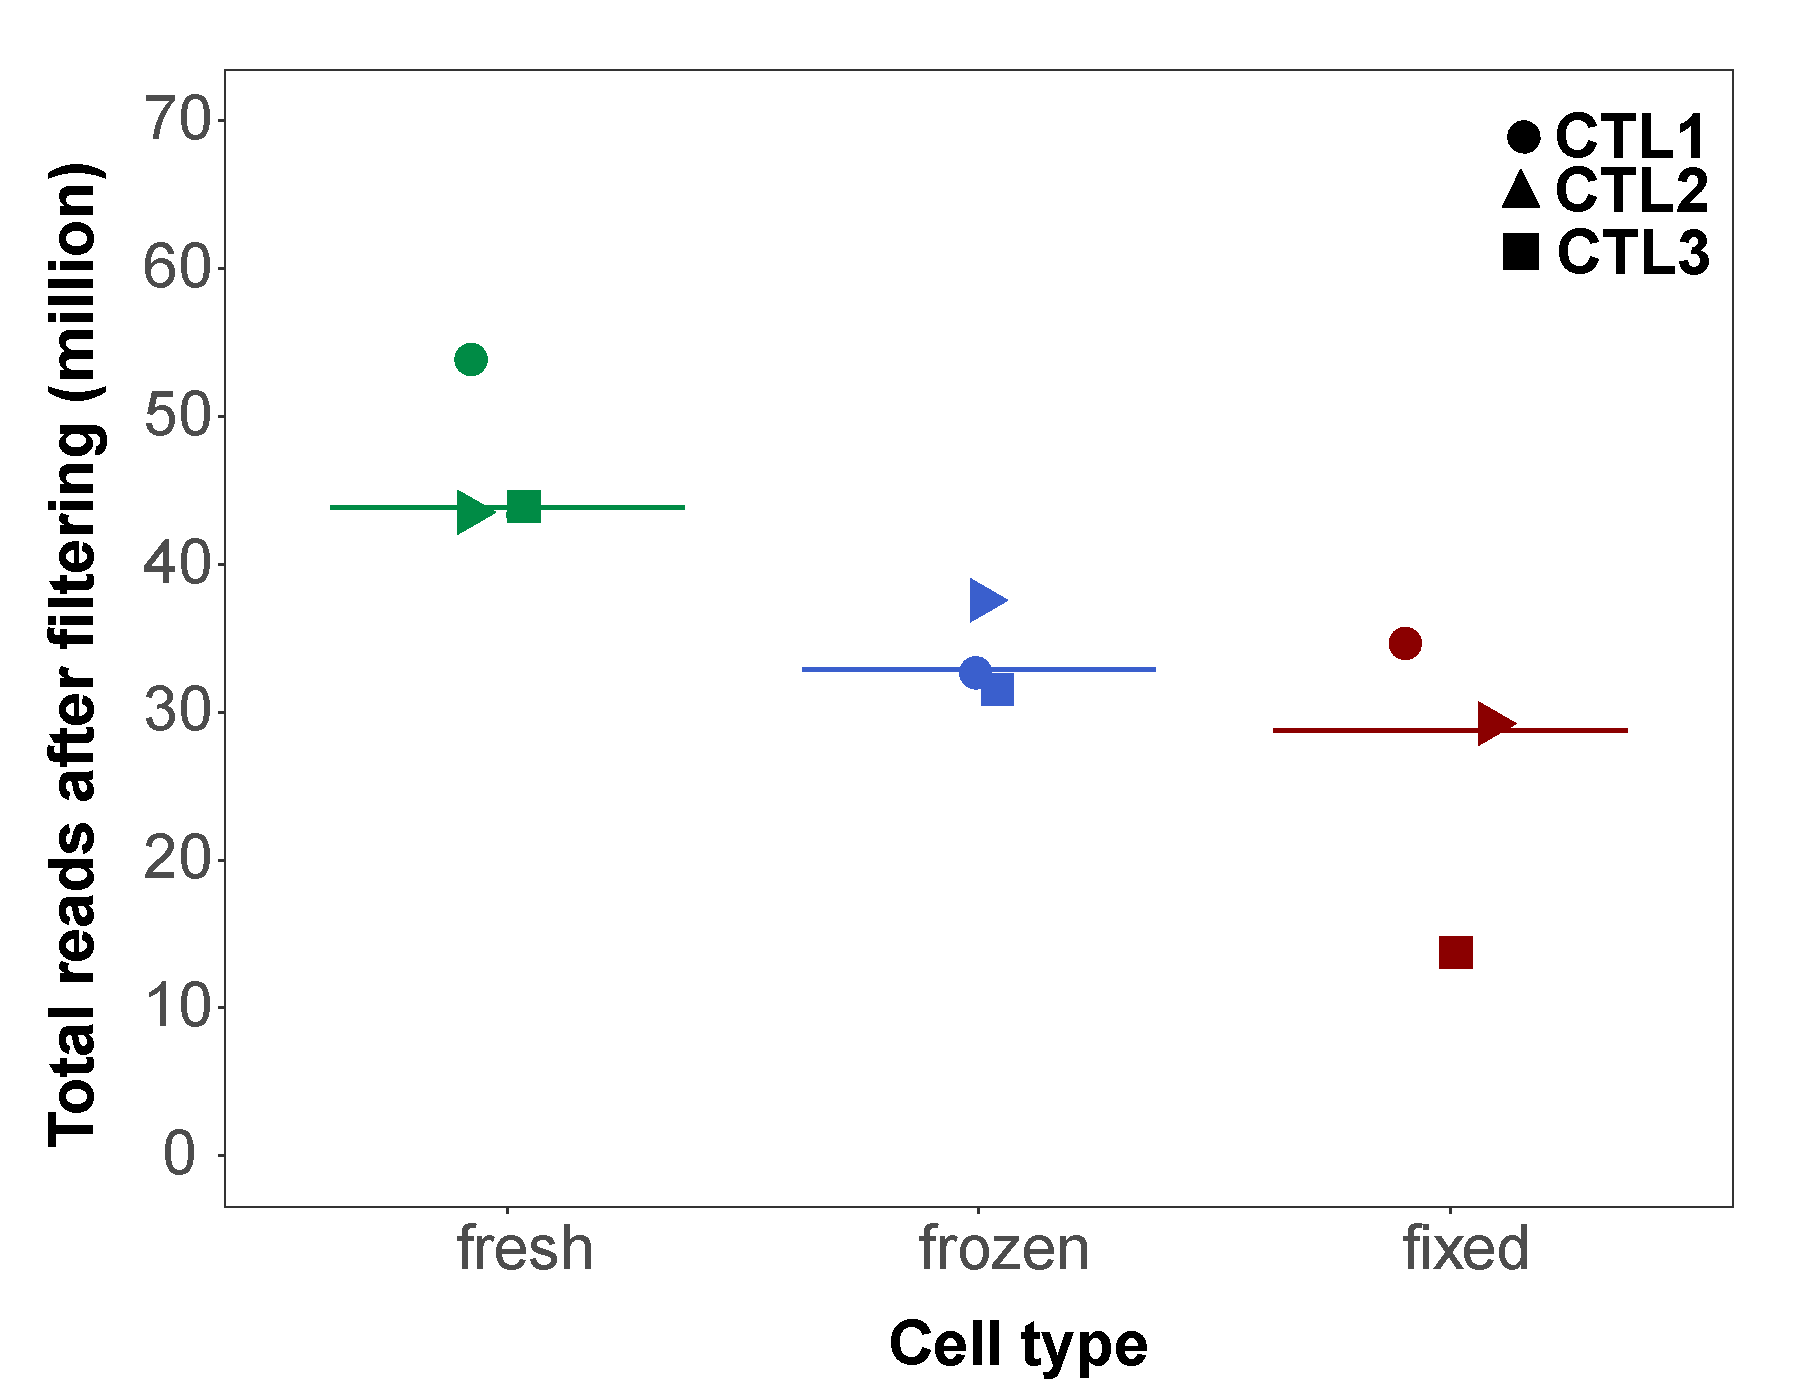
\includegraphics[width=\textwidth]{./Results1/pdfs/Core_ATAC_CD4_fresh_frozen_fixed_filtered_total_reads}
\caption{\textbf{}}
\end{subfigure}
\caption[Total number of ATAC-seq reads for the fresh, frozen and fixed CD14$^+$ monocytes and CD4$^+$ samples for 3 volunteers (CTL1-3).]{\textbf{Total number of ATAC-seq reads for the fresh, frozen and fixed CD14$^+$ monocytes and CD4$^+$ samples for 3 volunteers (CTL1-3).} Representation of million reads after filtering for the fresh, fixed and frozen ATAC-seq libraries in (A) CD14$^+$ monocytes and (B) CD4$^+$ cells.}
\label{figure:Core_ATAC_all_conditions_total_reads}
\end{figure} 

The ATAC-seq signal-to-noise ratios across the TSS showed a similar median for the fresh and fixed CD14$^+$ monocytes libraries (17.4 and 16.5 fold-enrichment, respectively) and was higher for the frozen samples (26.3 fold-enrichment)(Table \ref{tab:Core_ATAC_TSS_summary_table}). The median TSS enrichments in the frozen and fixed CD4$^+$ samples were considerably higher (16.1 and 14.3 fold-enrichment, respectively) than the fresh samples (5.6), which were borderline for the ENCODE recommended threshold. For one volunteer (CTL1) the fixed samples of both cell types showed considerably lower TSS enrichment (2.5 and 7.9, respectively) compared to the other fixed samples (Table \ref{tab:Core_ATAC_TSS_summary_table}). 


In terms of the fragment size distribution, the profiles of all the samples, except fixed CD14$^+$ monocytes and CD4$^+$ from CTL1, were similar, showing NFR $<$150bp and fragments corresponding to mono-, di-, tri- and tetra-nucleosomes (Figure \ref{figure:Core_ATAC_all_fragment_size_distribution} a and b). The fixed samples presented a lower density of NFF when compared to fresh and frozen, which had very similar distributions in both cell types. In particular, fixed CD14$^+$ monocytes and CD4$^+$ in CTL1 had extremely low abundance of NFF (Figure \ref{figure:Core_ATAC_all_fragment_size_distribution} red-dashed line in A and B), consistent with the very low TSS enrichment for CTL1 CD14$^+$ ATAC-seq fixed cells, as previously highlighted. 

\begin{figure}[htbp]
\centering
\begin{subfigure}{0.5\textwidth}
\centering
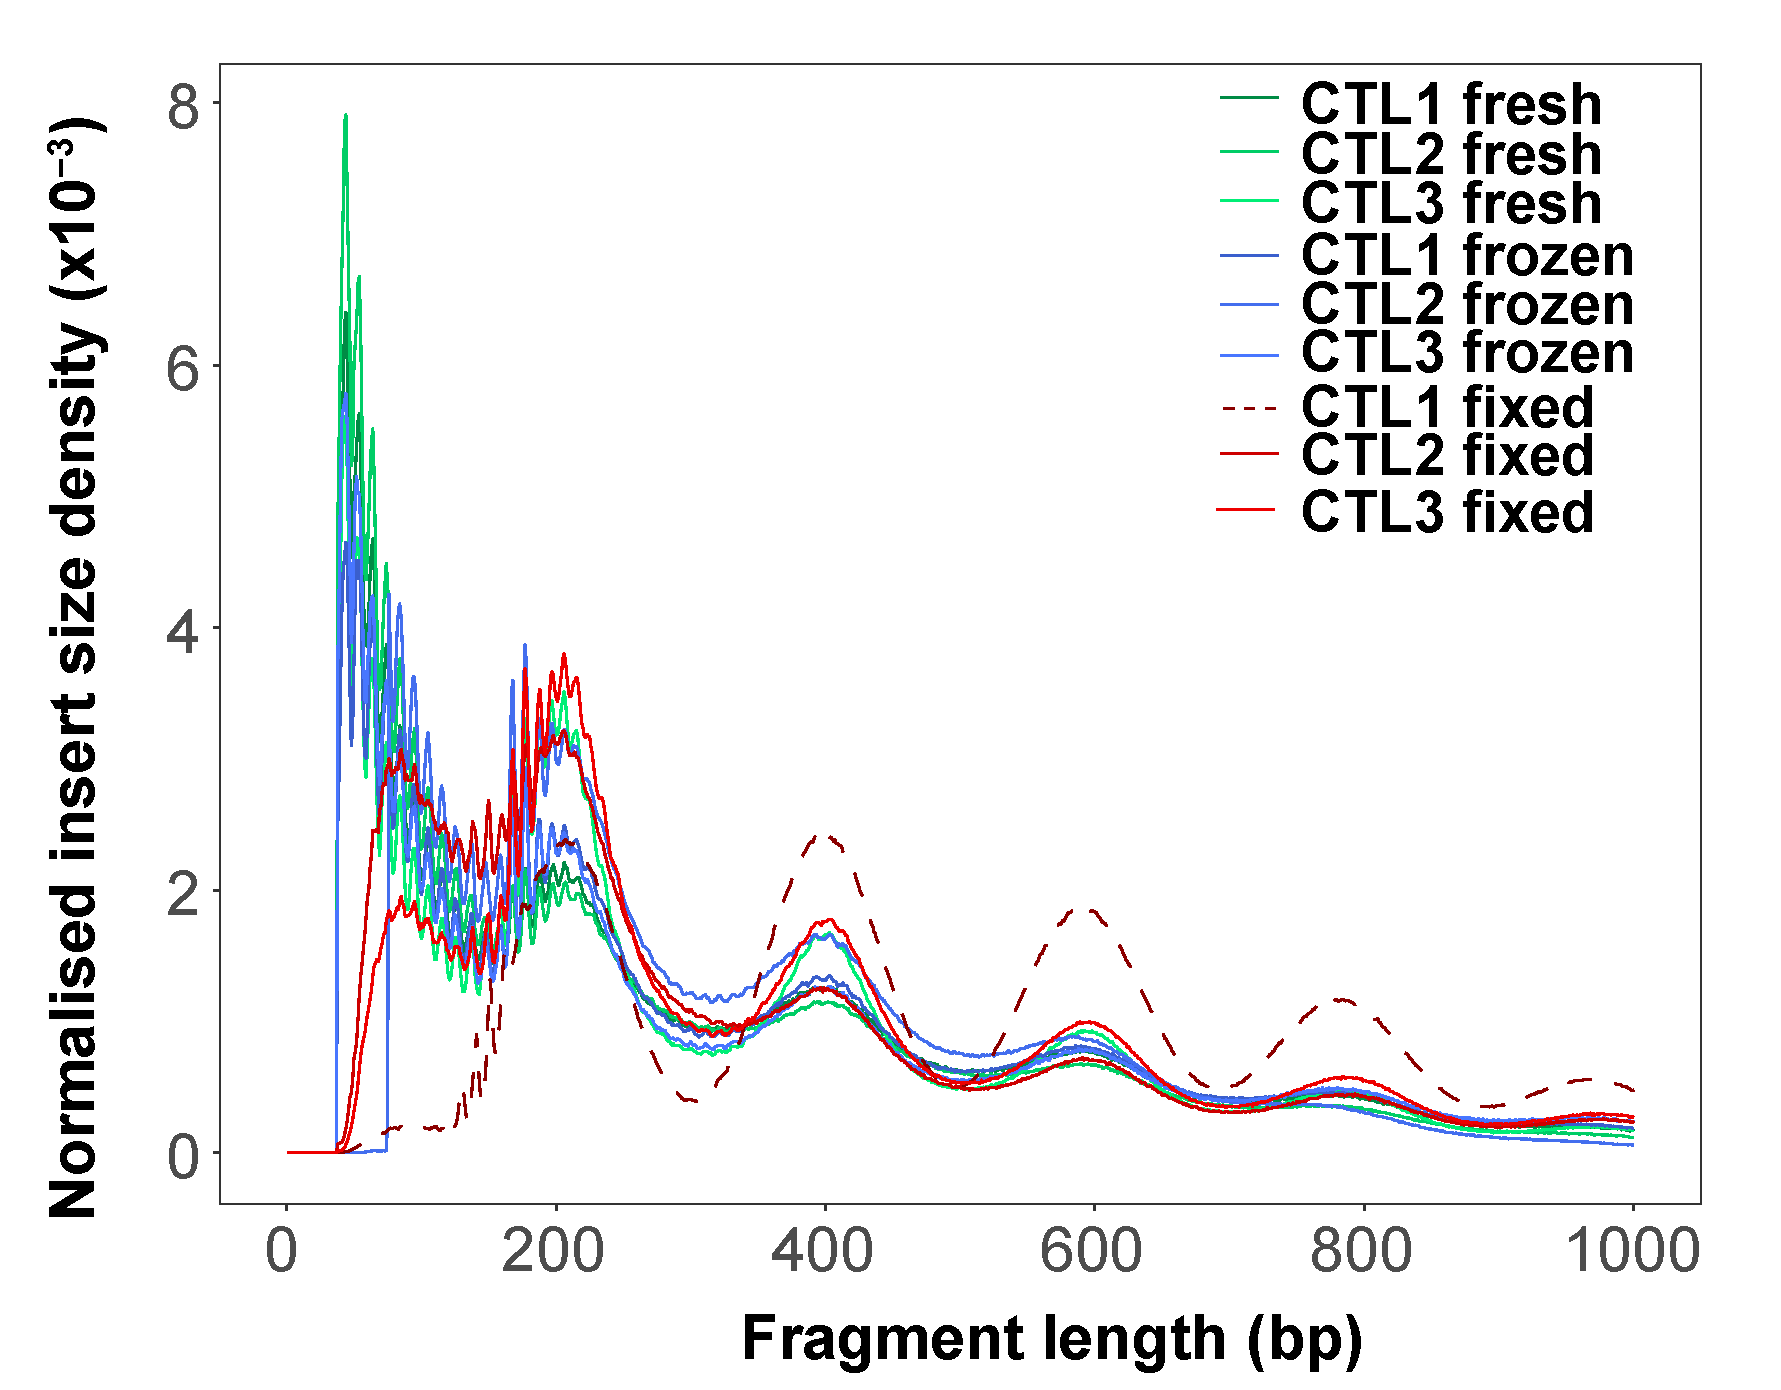
\includegraphics[width=\textwidth]{./Results1/pdfs/Core_ATAC_CD14_fresh_frozen_fixed_frag_size_distribution}
\caption{\textbf{}}
% The percentage sign indicated that the other subfig goes side by side
\end{subfigure}%
\begin{subfigure}{0.5\textwidth}
\centering
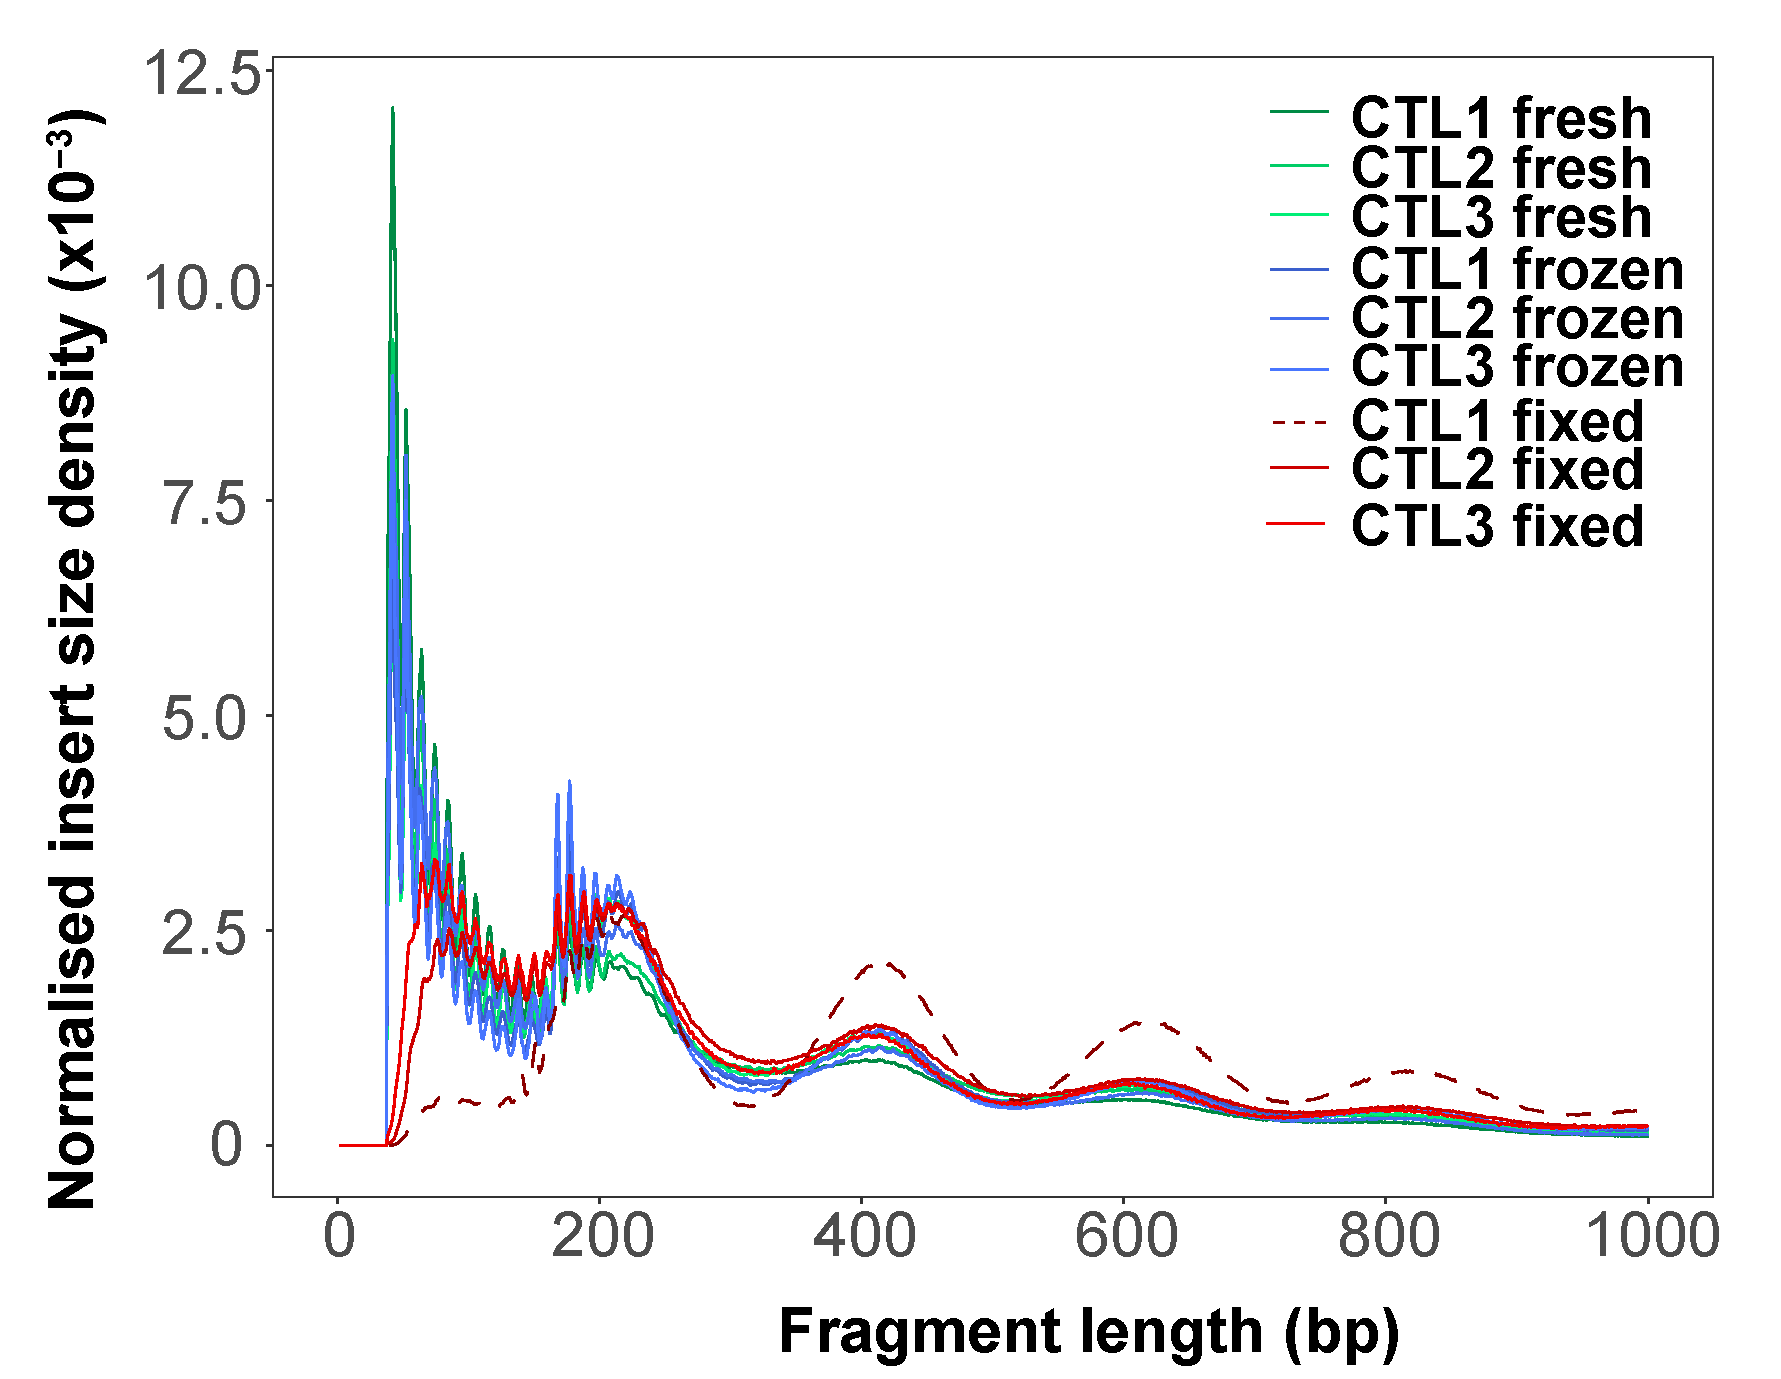
\includegraphics[width=\textwidth]{./Results1/pdfs/Core_ATAC_CD4_fresh_frozen_fixed_frag_size_distribution}
\caption{\textbf{}}
\end{subfigure}
\caption[Fragment size density distribution for ATAC-seq fresh, fixed and frozen in CD14$^+$ monocytes and CD4$^+$ cells.]{\textbf{Fragment size density distribution for ATAC-seq fresh, fixed and frozen in CD14$^+$ monocytes and CD4$^+$ cells.} The distribution of ATAC-seq fragment lengths are illustrated for (A) CD14$^+$ monocytes and (B) CD4$^+$ cells and colour-coded by condition (fresh=green, frozen=blue and fixed=red).}
\label{figure:Core_ATAC_all_fragment_size_distribution}
\end{figure} 



Chromatin structure across and within the TSS was then investigated following Scharer and colleagues \parencite{Scharer2016}. The nucleosome-free fragments ($<$150bp) from all the samples showed a single peak of enrichment at the nucleosome-depleted TSS position, with CD4$^+$ fresh samples presenting the lowest enrichment (Figure \ref{figure:Core_ATAC_intra_dinucleosome_tss_enrichment}A and C). The pattern of enrichment of di-nucleosome fragments (ranging between 260 and 340bp) demonstrated in the majority of the samples a characteristic periodicity in the TSS surroundings, with two peaks of enrichment mapping at the up-stream and down-stream positioned nucleosomes (Figure \ref{figure:Core_ATAC_intra_dinucleosome_tss_enrichment}B and D). 

%This pattern of enrichment was weaker in the three fresh samples from CD4$^+$ and absent in the CTL1 CD14$^+$ fixed sample. The fresh CD4$^+$ samples also presented low enrichment for the nucleosome-free fragments in the TSS, similar to their overall TSS enrichment (Table \ref{tab:Core_ATAC_TSS_summary_table}) but still weakly identified the position of the two nucleosomes in the TSS surroundings, suggesting an overall preservation of the chromatin structure. 



\begin{figure}[H]
\centering
\begin{subfigure}[b]{0.45\textwidth}
\centering 
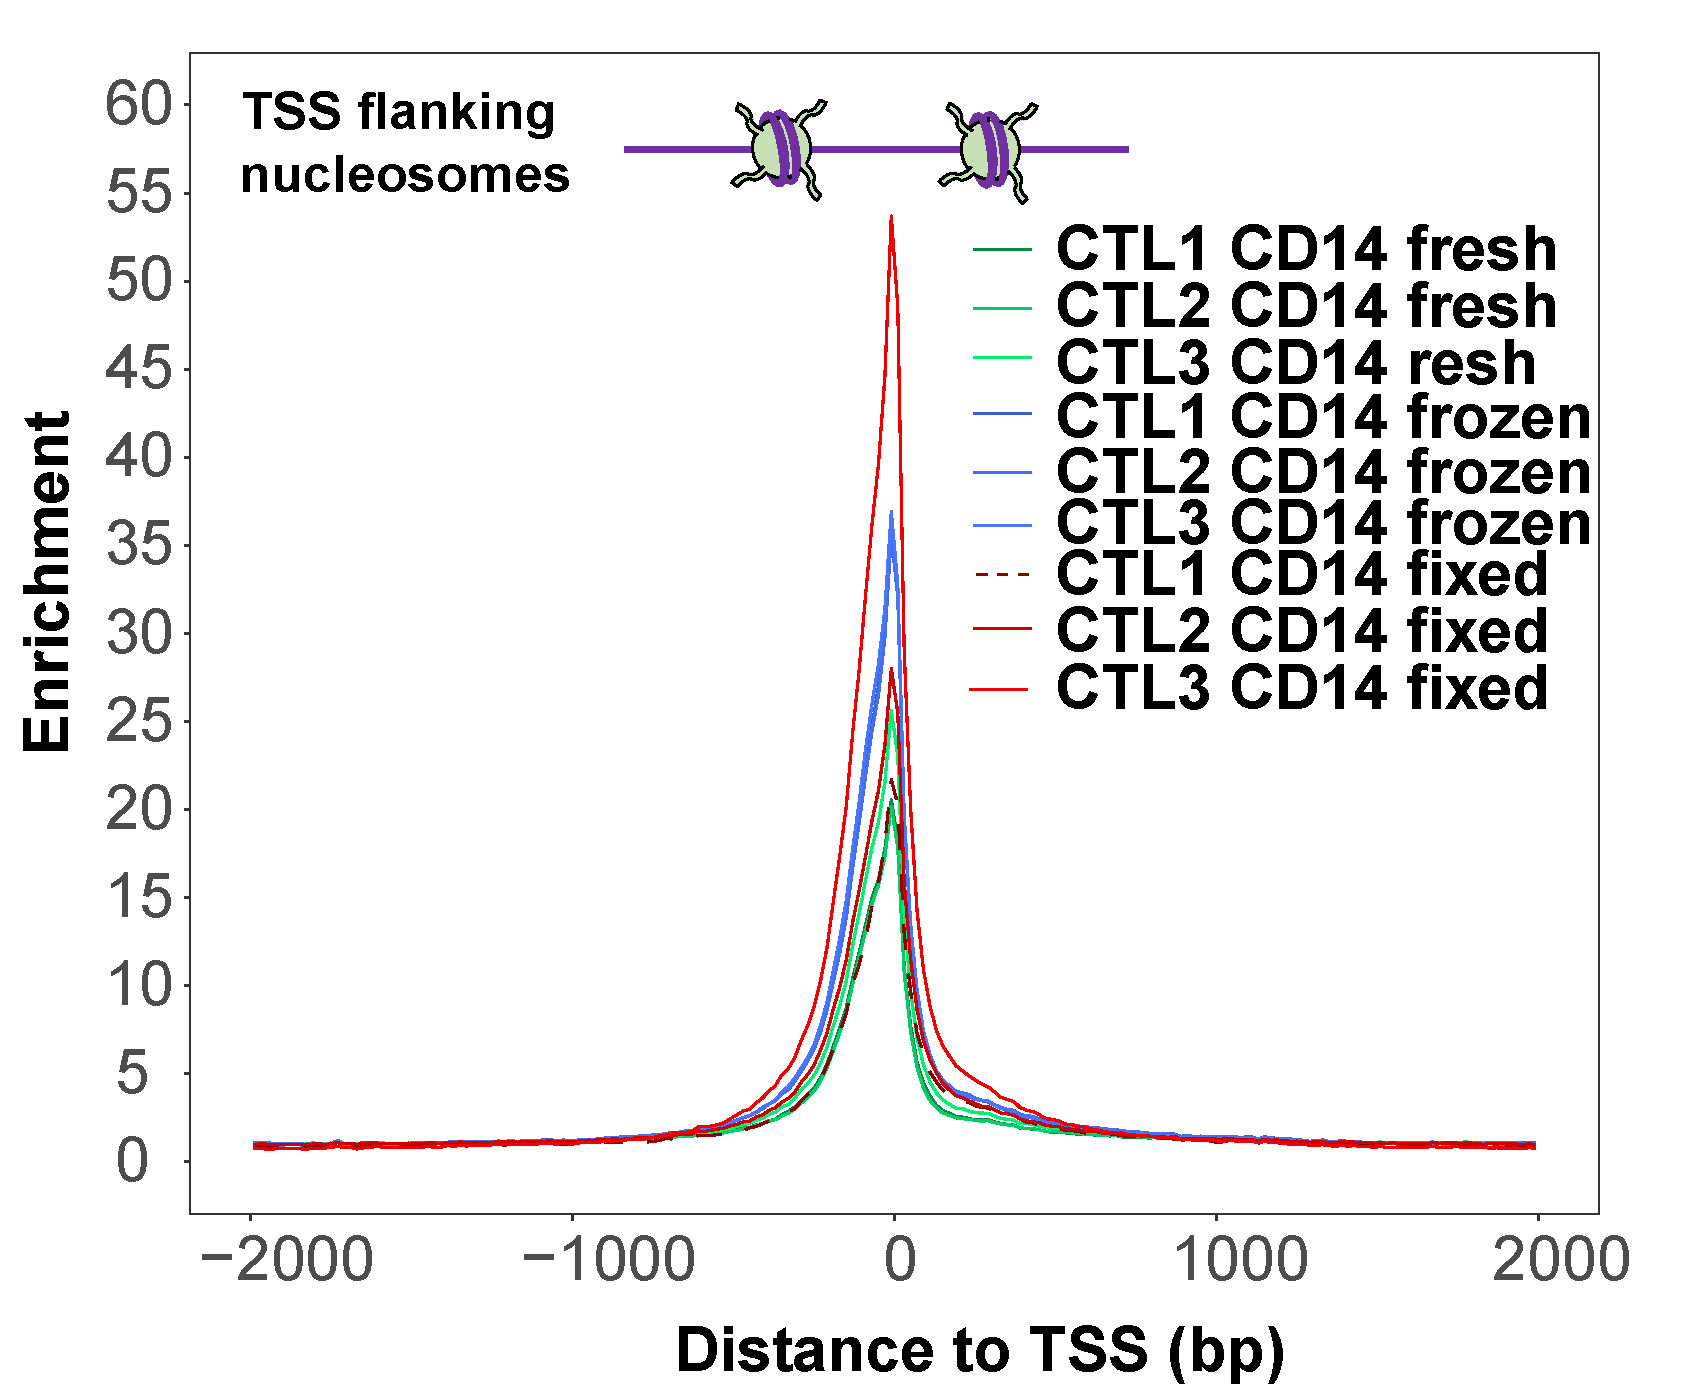
\includegraphics[width=\textwidth]{./Results1/pdfs/Core_ATAC_CD14_fresh_frozen_fixed_internucleosome_TSS}
\caption{}
\end{subfigure}
~
\begin{subfigure}[b]{0.45\textwidth}
\centering 
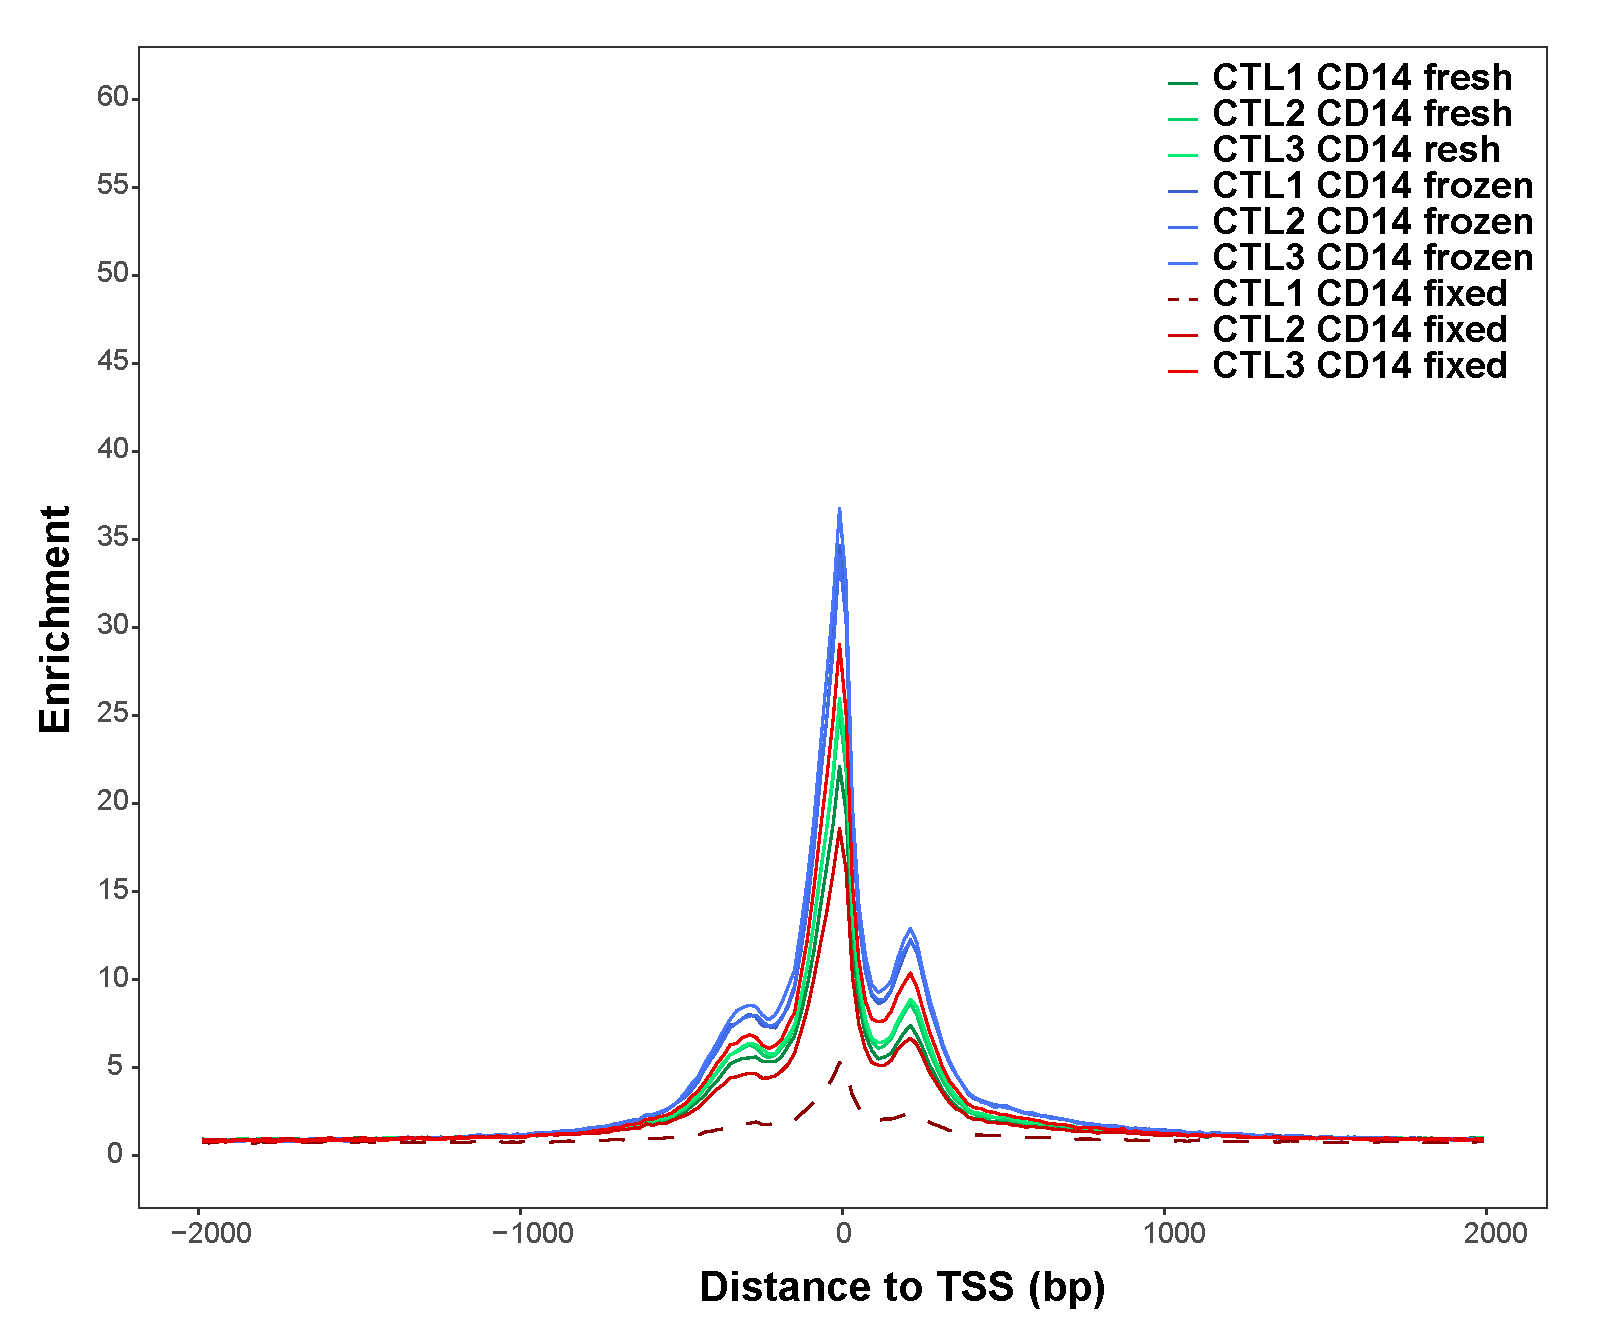
\includegraphics[width=\textwidth]{./Results1/pdfs/Core_ATAC_CD14_fresh_frozen_fixed_dinucleosome_TSS}
\caption{}
\end{subfigure}
~
\begin{subfigure}[b]{0.45\textwidth} 
%the [b] prevents offset in subcaptions
\centering
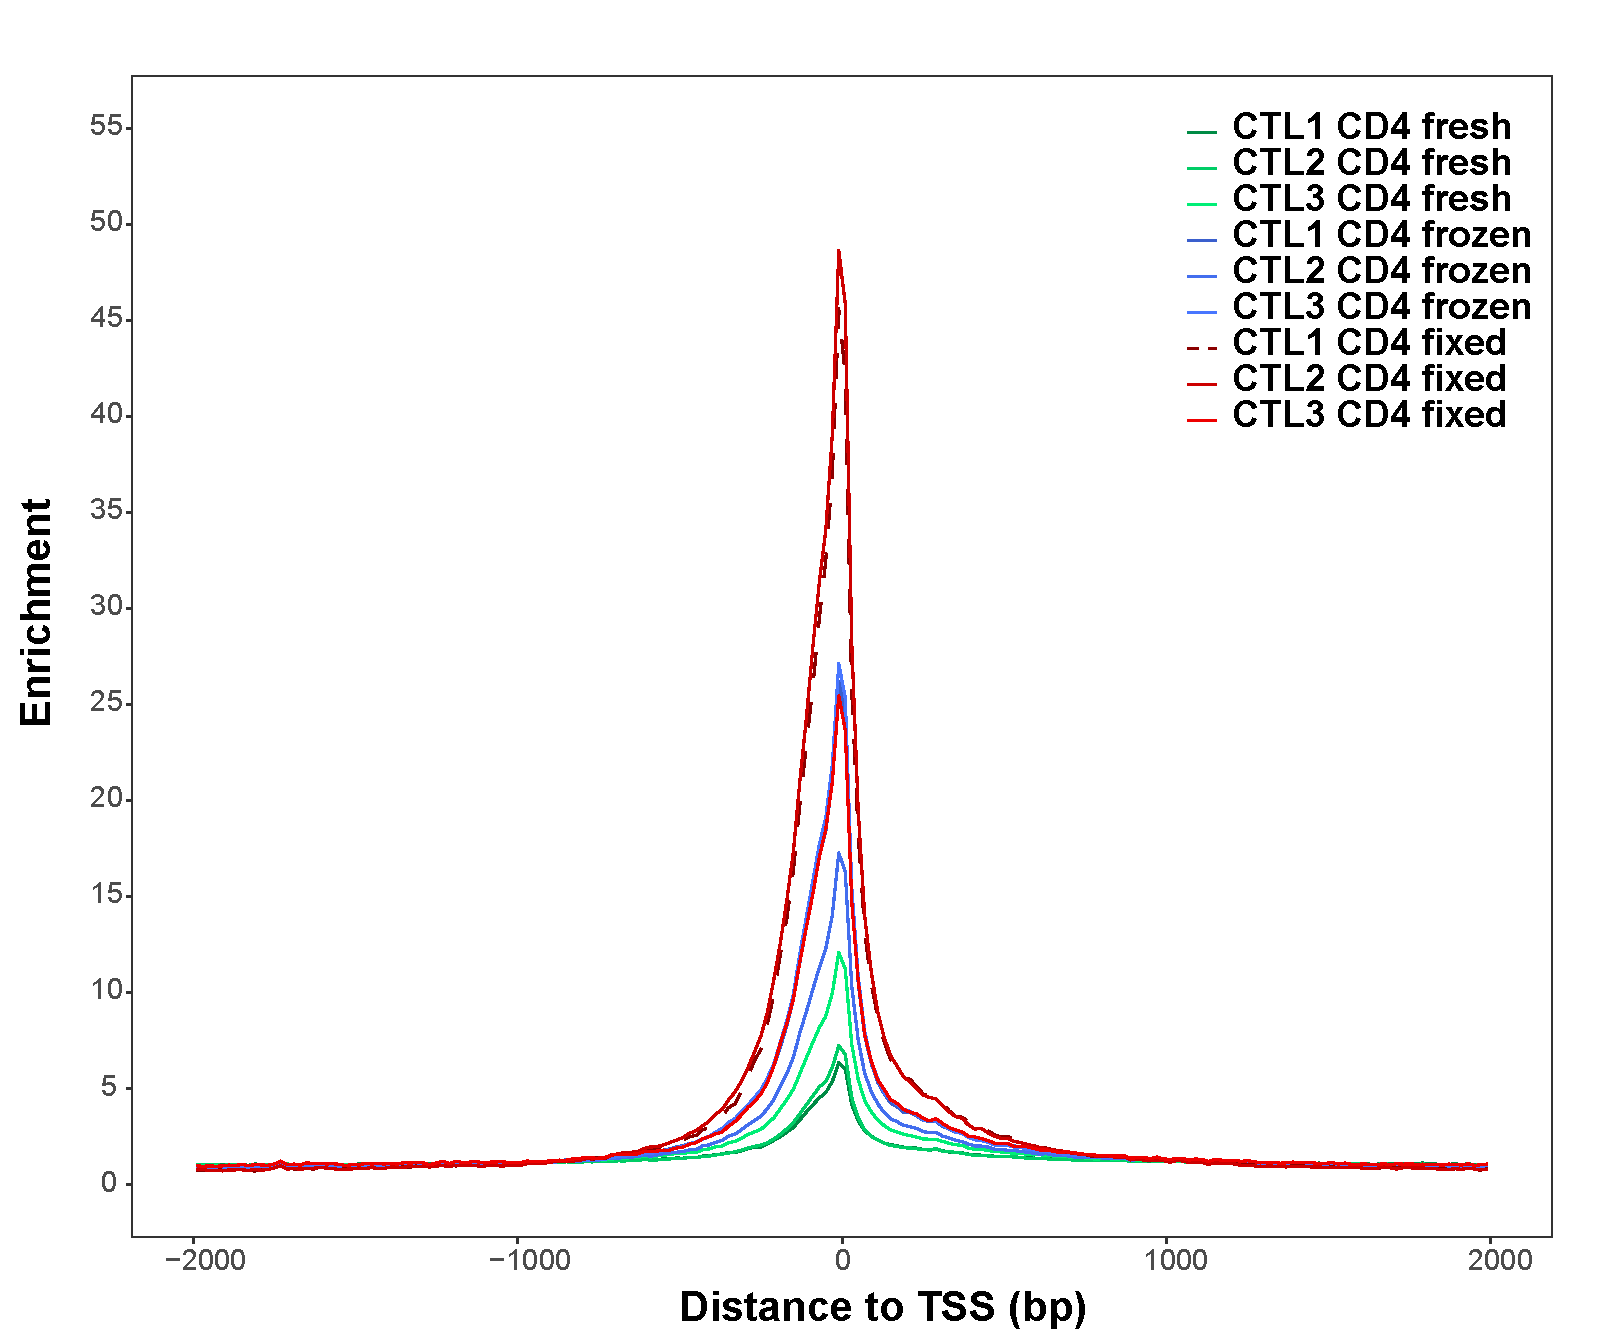
\includegraphics[width=\textwidth]{./Results1/pdfs/Core_ATAC_CD4_fresh_frozen_fixed_internucleosome_TSS}%
\caption{}
\end{subfigure}
\begin{subfigure}[b]{0.45\textwidth} 
%the [b] prevents offset in subcaptions
\centering
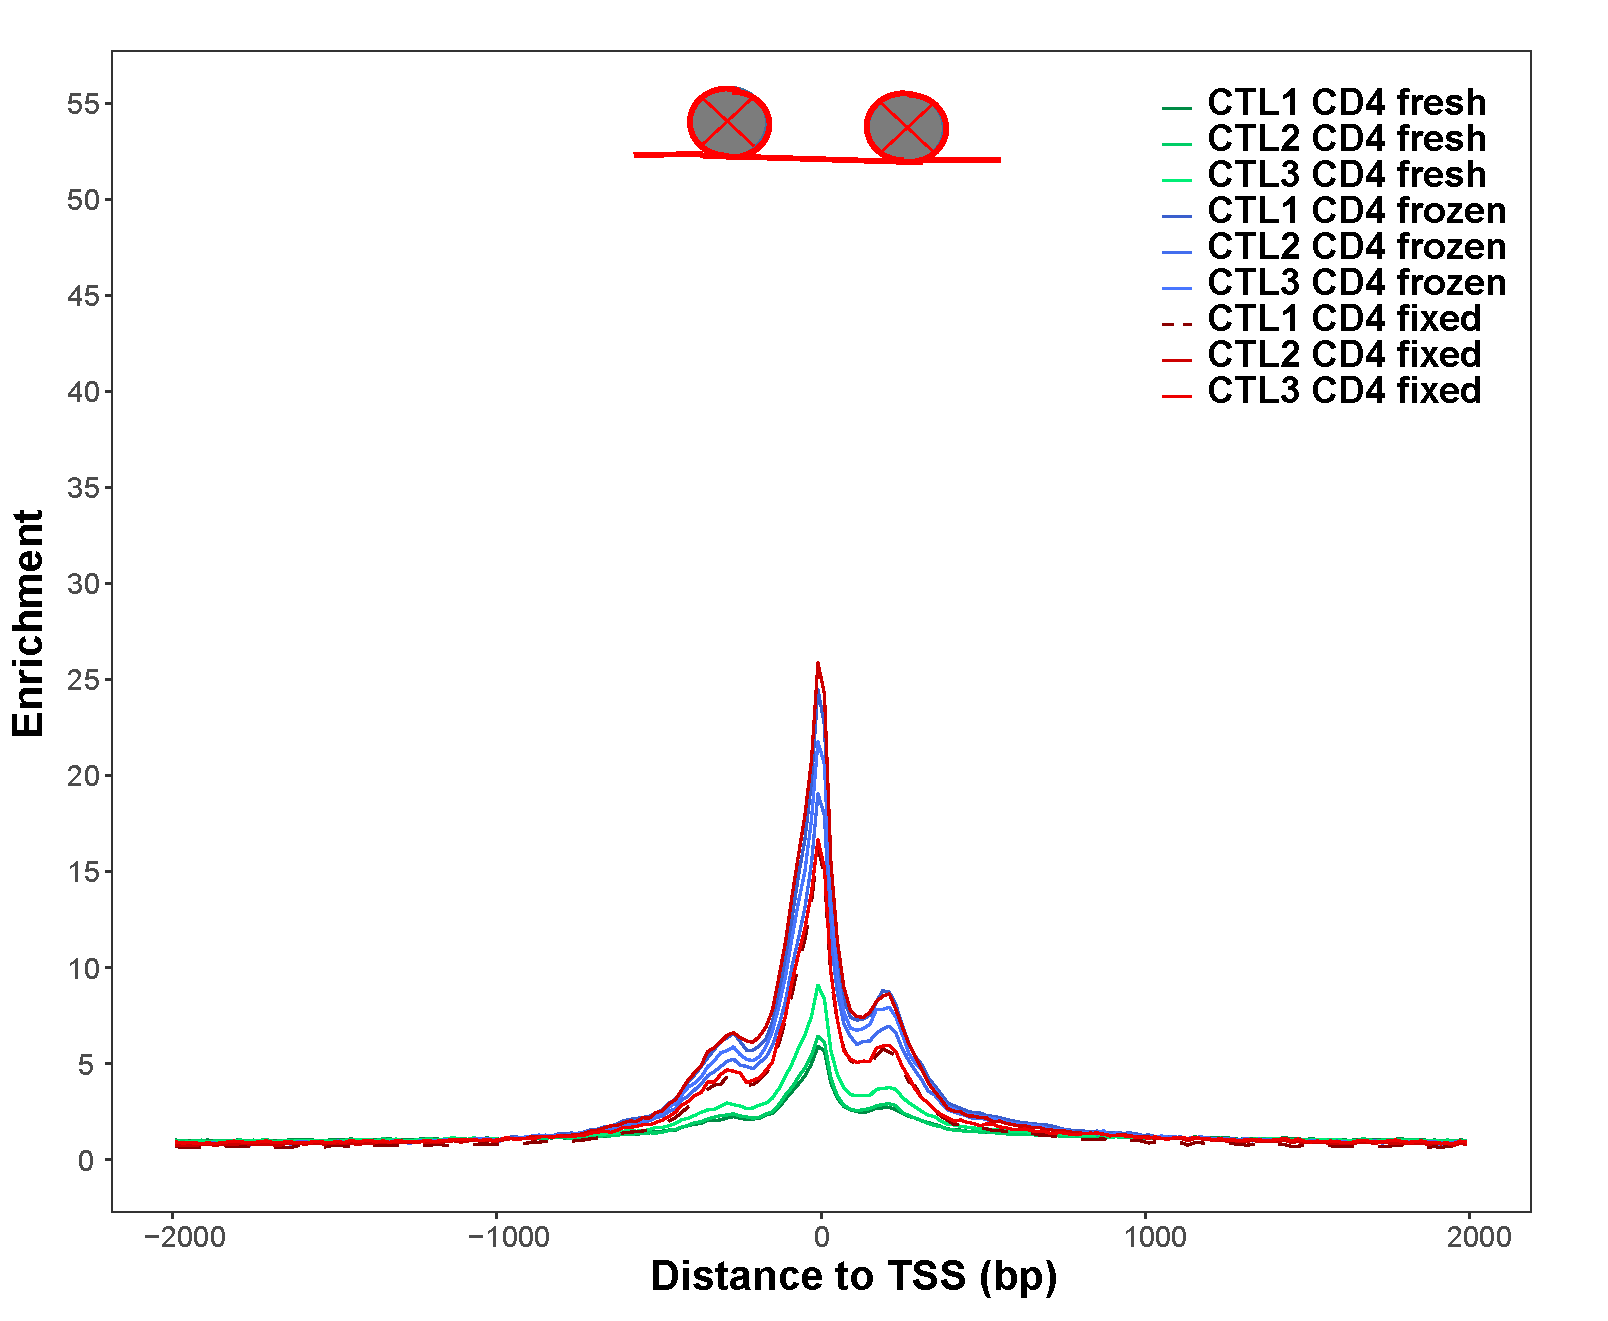
\includegraphics[width=\textwidth]{./Results1/pdfs/Core_ATAC_CD4_fresh_frozen_fixed_dinucleosome_TSS}%
\caption{}
\end{subfigure}
\caption[ATAC-seq enrichment of nucleosome-free and di-nucleosome fragments at the TSS and surroundings in CD14$^+$ monocytes and CD4$^+$ samples for the three conditions.]{\textbf{ATAC-seq enrichment of nucleosome-free and di-nucleosome fragments at the TSS and surroundings in CD14$^+$ monocytes and CD4$^+$ samples for the three conditions.} Nucleosome-free fragments ($<$150bp) and di-nucleosome (between 260 and 340bp) were selected \textit{in silico} and enrichment analysis was carried out $+/-$1Kb across all the Ensembl annotated TSS.}
\label{figure:Core_ATAC_intra_dinucleosome_tss_enrichment}
\end{figure}


Although fixation in CTL1 CD14$^+$ reduced the abundance of nucleosome-free tagged fragments, the ATAC-seq signal at those regions was clearly enriched when compared to the background. In contrast, DSP in CTL1 CD14$^+$ appeared to increase the efficiency of ATAC-seq in tagging NBF (di-, tri- and tetra-nucleosomes) but the loss of chromatin structure around the TSS indicated that those fragments are likely to have been displaced from their original location. Conversely, the fresh CD4$^+$ samples showed low enrichment for NFF in the TSS, in line with their overall TSS enrichment (Table \ref{tab:Core_ATAC_TSS_summary_table}) and indicating weakly the two nucleosome positioned in the TSS surroundings. In summary, freezing and, importantly fixing (with exception of the two cell types from CTL1) appeared to maintain the overall chromatin structure.

Annotation of the significant peaks from each sample (filtered for the optimal IDR p-value as explained in \ref{peak_filtering}) revealed that the highest proportion of ATAC-seq peaks localised to promoters, introns and intergenic regions (Figure \ref{figure:Core_ATAC_all_conditions_genomic_features}A and B), consistent with previous studies \parencite{Buenrostro2013,Scharer2016}. The higher percentage of peaks annotated as promoters for some ATAC-seq libraries revealed the preferential location of strong good quality peaks at this feature when compared to other genomic features. Overall, the genomic annotation of the peaks across the three conditions revealed accessible ATAC-seq regions at meaningful genomic features. 

\begin{figure}[htbp]
\centering
\begin{subfigure}{0.5\textwidth}
\centering
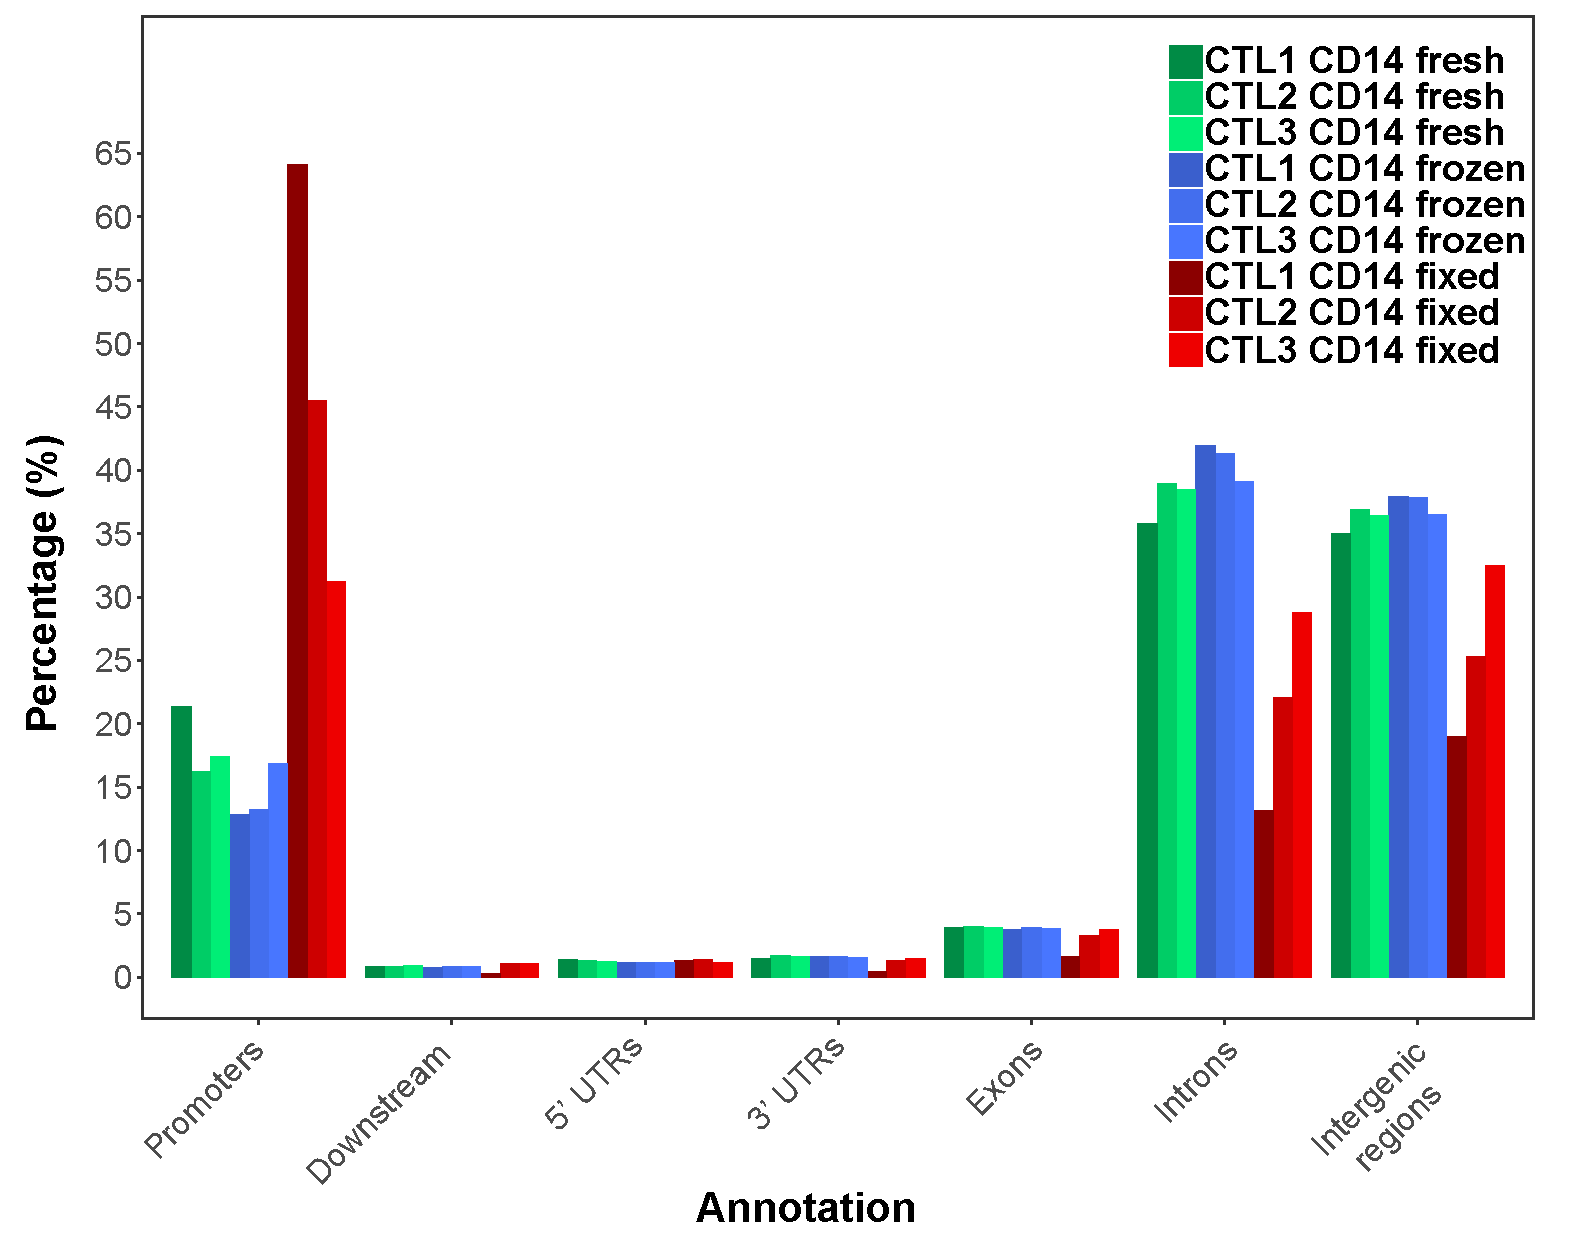
\includegraphics[width=\textwidth]{./Results1/pdfs/Core_ATAC_CD14_fresh_frozen_fixed_IDR_filtered_peak_annotation}
\caption{\textbf{}}
% The percentage sign indicated that the other subfig goes side by side
\end{subfigure}%
\begin{subfigure}{0.5\textwidth}
\centering
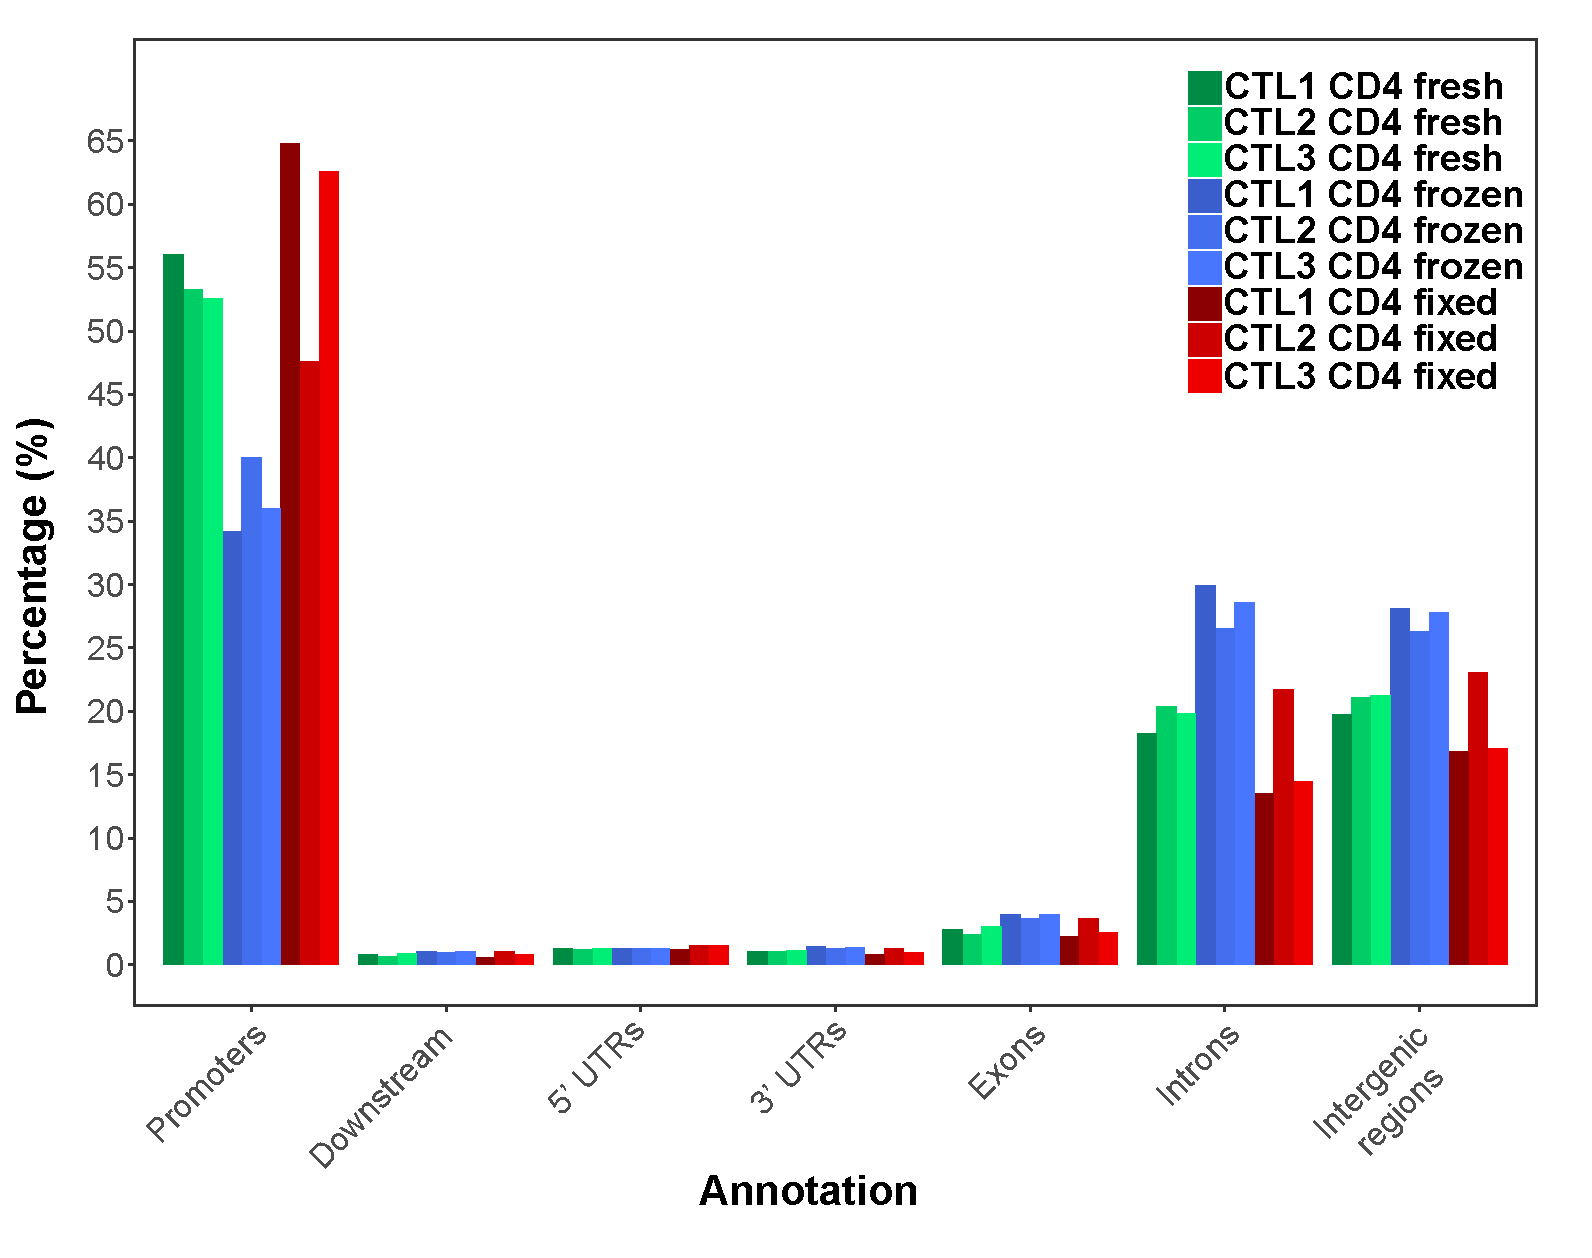
\includegraphics[width=\textwidth]{./Results1/pdfs/Core_ATAC_CD4_fresh_frozen_fixed_IDR_filtered_peak_annotation}
\caption{\textbf{}}
\end{subfigure}
\caption[Genomic features annotation for the ATAC-seq peaks called in each of the fresh,frozen and fixed samples from CD14$^+$ monocytes and total CD4$^+$.]{\textbf{Genomic features annotation for the ATAC-seq peaks called in each of the fresh,frozen and fixed samples from CD14$^+$ monocytes and CD4$^+$.} Overlap was performed between the genomic features and the list of (A)CD14$^+$ monocytes and (B) CD4$^+$ peaks filtered for FDR$<$0.01 in each sample from each of the three conditions (fresh=green, frozen=blue and fixed=red).}
\label{figure:Core_ATAC_all_conditions_genomic_features}
\end{figure} 


\subsubsection{Differential analysis demonstrates discrete significant changes in chromatin accessibility across conditions}
In order to investigate genome wide differences between ATAC-seq fresh (biological reference) and ATAC-seq frozen and fixed, read counts were retrieved at the peaks from a consensus master list including the three conditions for each cell type (ML\_CD14\_all\_cond and ML\_CD14\_all\_cond). For this analysis the data relating toCTL1 fixed samples from CD14$^+$ and CD4$^+$ cells were removed given the low quality metrics previously described. 
     
\begin{figure}[htbp]
\centering
\begin{subfigure}{0.5\textwidth}
\centering
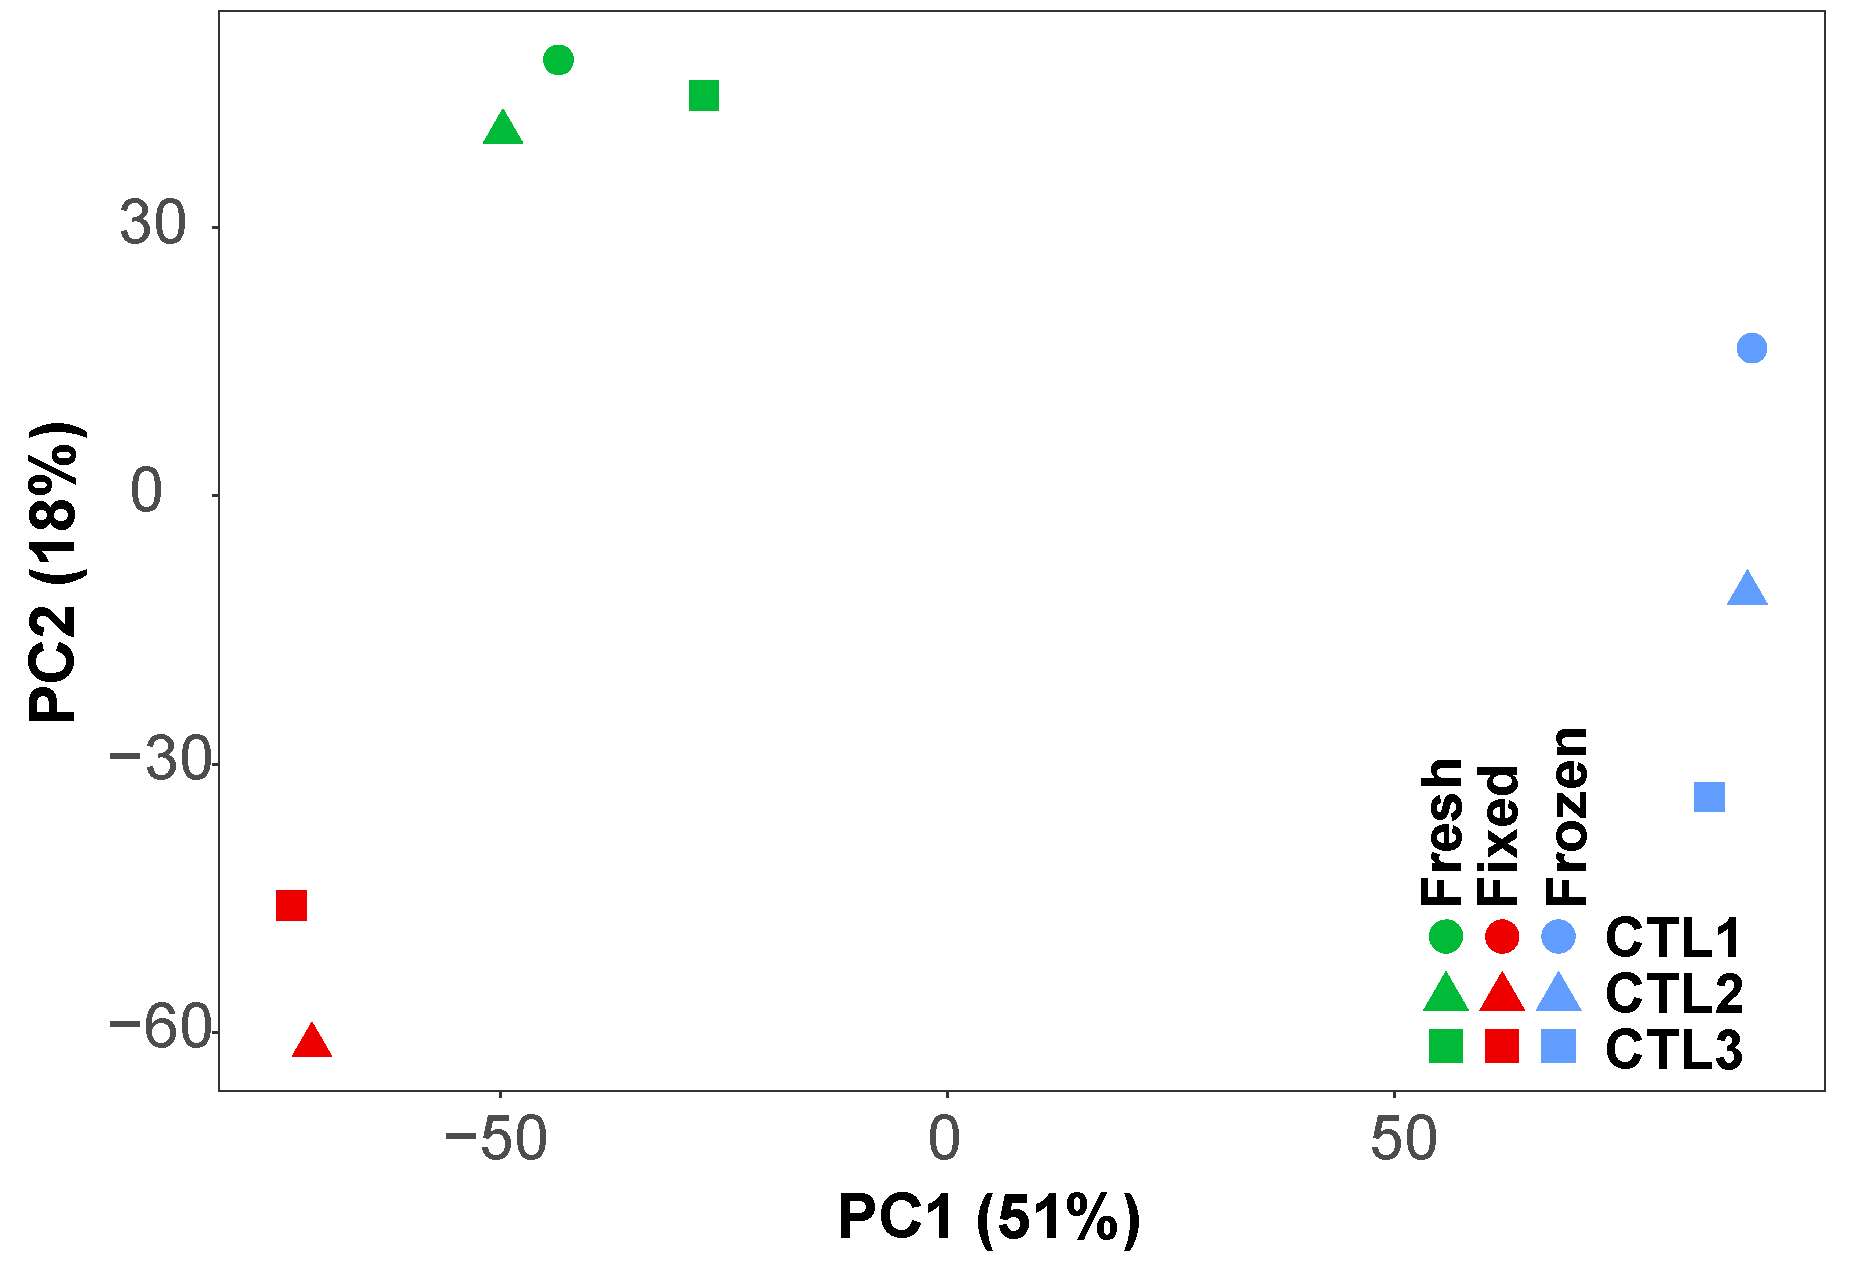
\includegraphics[width=\textwidth]{./Results1/pdfs/Core_ATAC_CD14_fresh_frozen_fixed_no_CTL1_fixed_PCA}
\caption{\textbf{}}
% The percentage sign indicated that the other subfig goes side by side
\end{subfigure}%
\begin{subfigure}{0.5\textwidth}
\centering
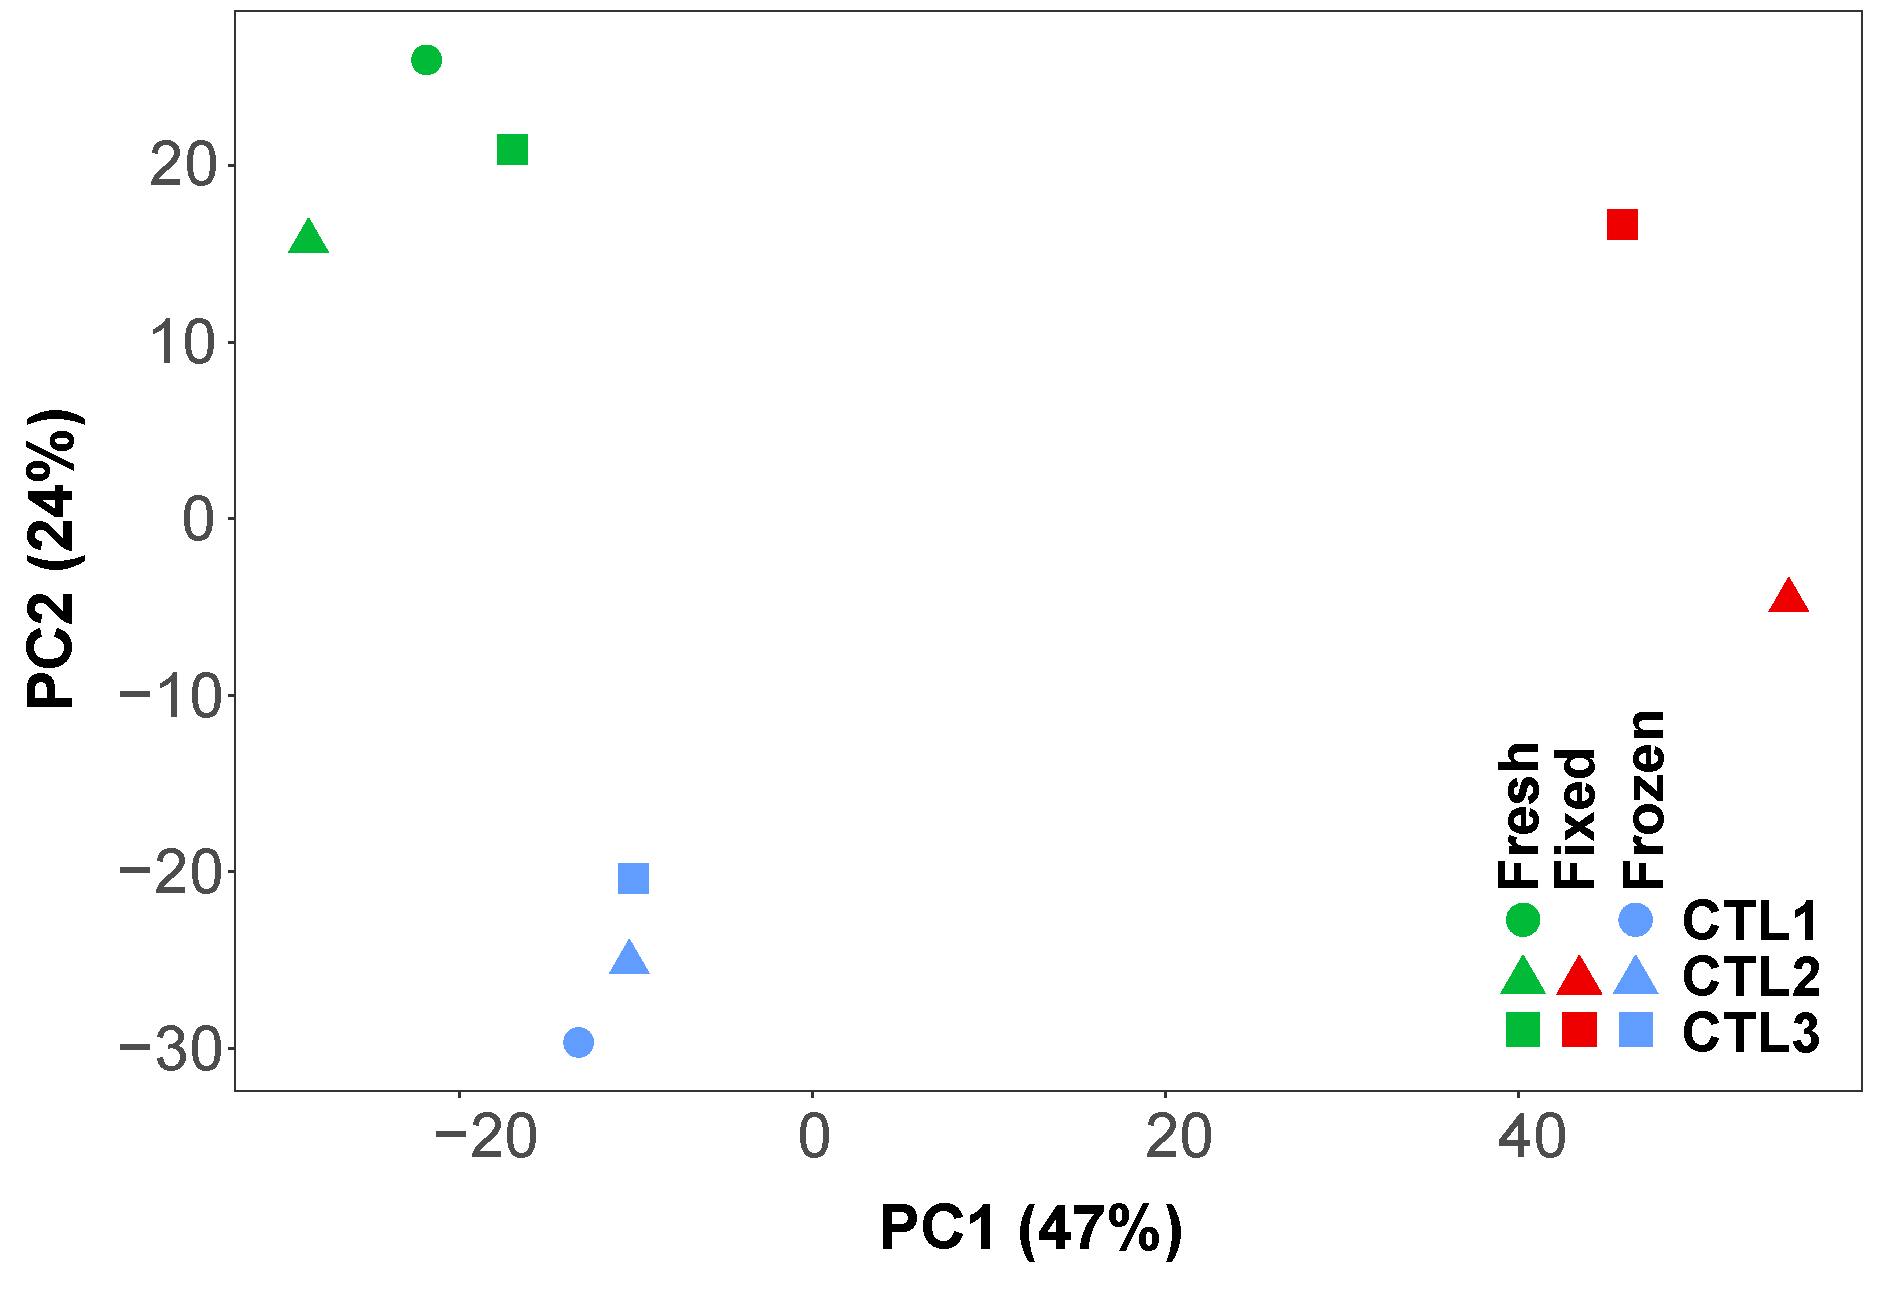
\includegraphics[width=\textwidth]{./Results1/pdfs/Core_ATAC_CD4_fresh_frozen_fixed_no_CTL1_fixed_PCA}
\caption{\textbf{}}
\end{subfigure}
\caption[PCA analysis based on the ATAC-seq chromatin accessibility landscape in fresh, fixed and frozen samples.]{\textbf{PCA analysis based on the ATAC-seq chromatin accessibility landscape in fresh, fixed and frozen samples.} PCA analysis was performed using the normalised counts across the consensus master list of the combined fresh, fixed and frozen samples (ML\_CD14\_all\_cond and ML\_CD4\_all\_cond) in (A) CD14$^+$ monocytes or (B) CD4$^+$ cells from the same three healthy individuals. The first two PCs (x-axis and y-axis, respectively) of all the regions included in each of the master lists are plotted. Each point represents a sample, where shape codes for individual (CTL1, CTL2, CTL3) and colour means condition (fresh, fixed, frozen). The proportion of variation explained by each principal component is indicated.}
\label{figure:Core_ATAC_all_conditions_PCA}
\end{figure}



Principal component analysis (PCA) was performed using DESeq2 normalised counts for each of the two master lists demonstrated differences across the three ATAC-seq conditions in the two cell types. Plotting the first two principal components (PCs) showed sample clustering based on condition, which explained the largest variability within the two cell types. The first PC explaining 51\% of the variance in the chromatin accessibility landscape across samples, separated ATAC-seq fresh and fixed from the ATAC-seq frozen samples in CD14$^+$ monocytes (Figure \ref{figure:Core_ATAC_all_conditions_PCA}A). The second PC (16\% of variance) showed more moderate changes between fresh and fixed libraries. In contrast, PCA analysis in CD4$^+$ showed fixed to present the largest differences versus fresh in the genome-wide accessibility (Figure \ref{figure:Core_ATAC_all_conditions_PCA}B). 


To further compare chromatin accessibility across the three conditions, the normalised read counts at each of the ML\_CD14\_all\_cond and ML\_CD4\_all\_cond master lists peaks were contrasted between fresh and fixed or frozen. The majority of the regions showed highly correlated ATAC-seq normalised counts between fresh and frozen or fixed, with the lowest correlation (R=0.918) found between fresh and frozen CD14$^+$ monocytes (Figure \ref{figure:Core_ATAC_all-conditions_correlation}A, B, C and D). 


\begin{figure}[H]
\centering
\begin{subfigure}[b]{0.45\textwidth}
\centering 
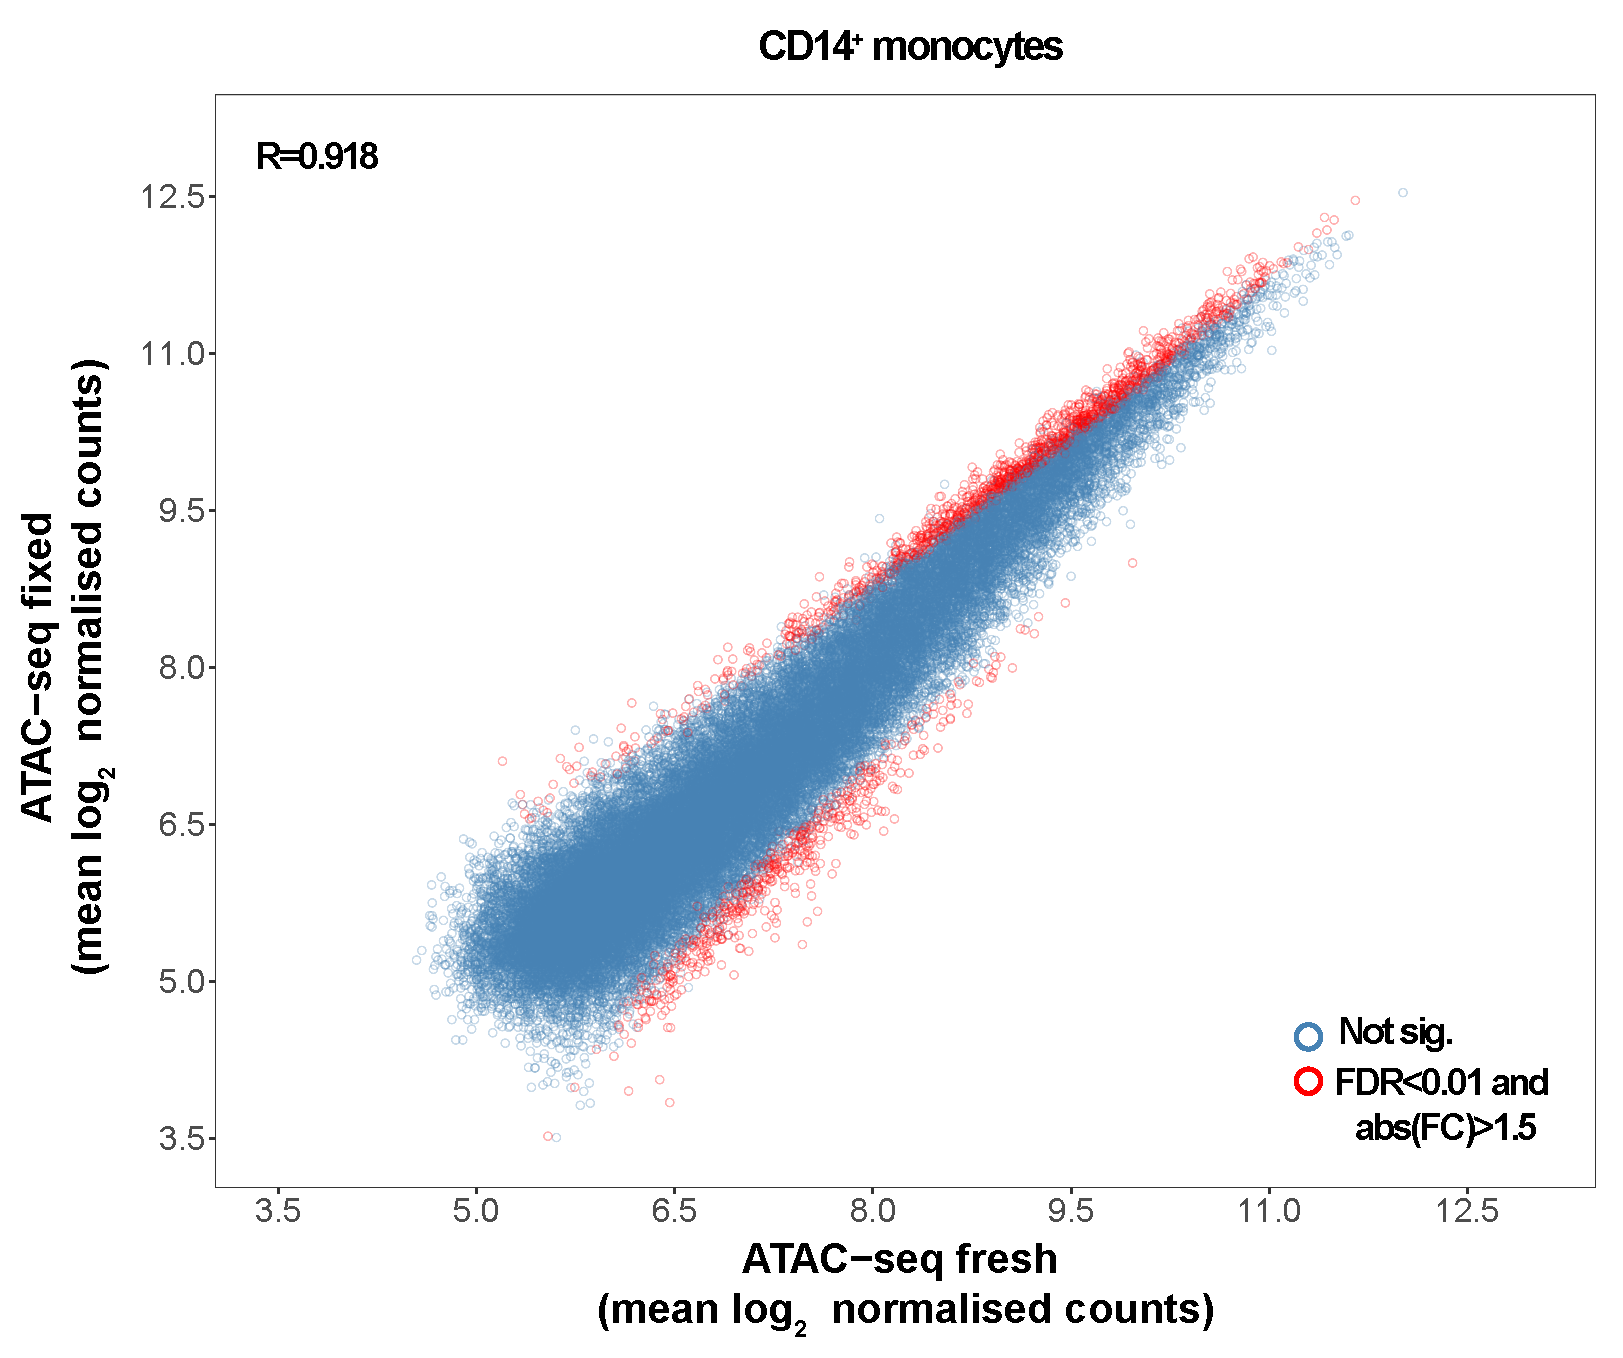
\includegraphics[width=\textwidth]{./Results1/pdfs/Core_ATAC_CD14_fresh_fixed_correlation_counts_small}
\caption{}
\end{subfigure}
~
\begin{subfigure}[b]{0.45\textwidth}
\centering 
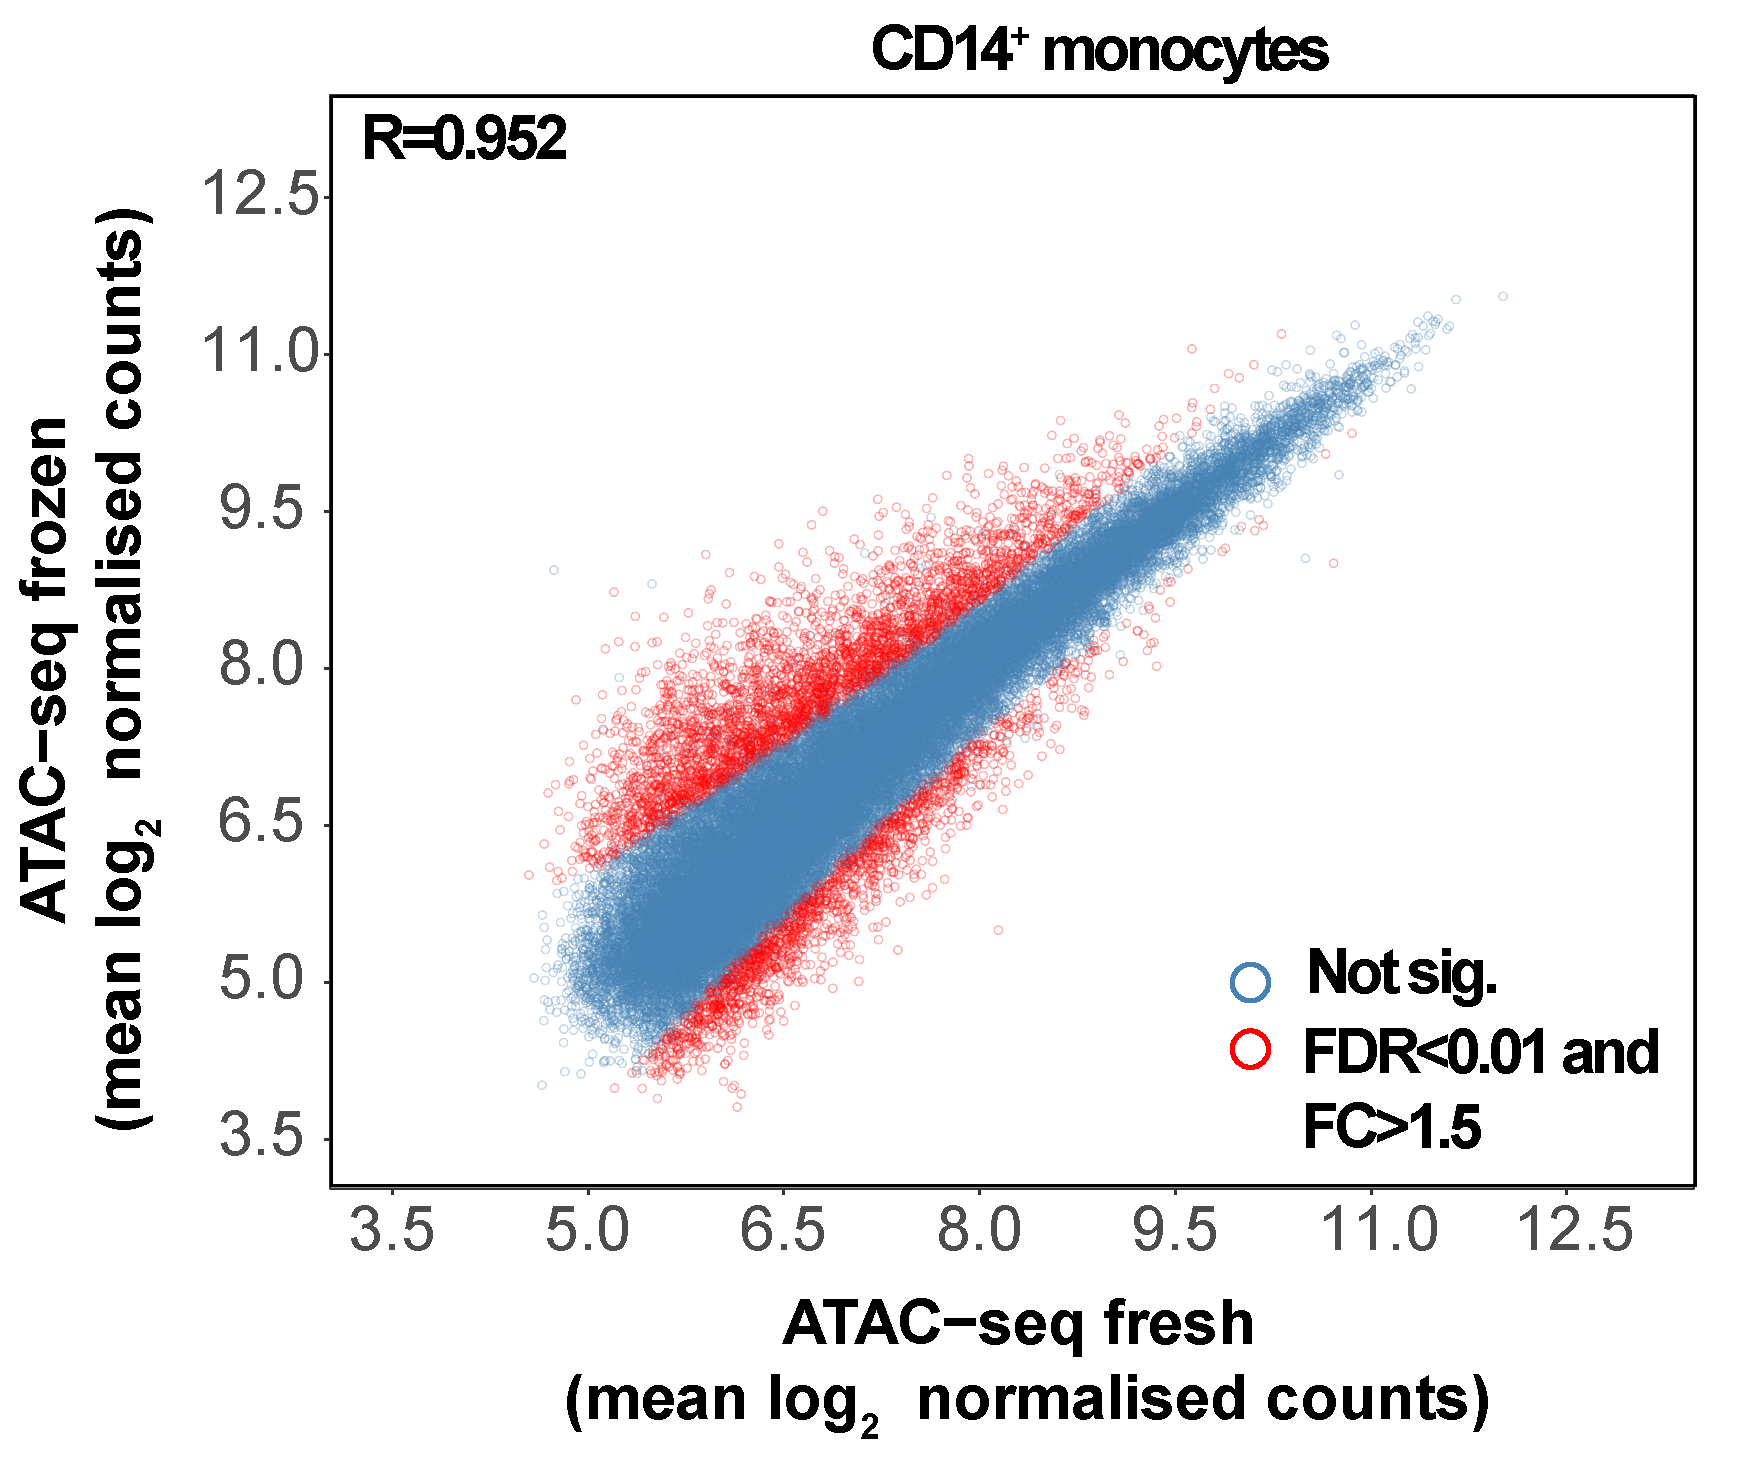
\includegraphics[width=\textwidth]{./Results1/pdfs/Core_ATAC_CD14_fresh_frozen_correlation_counts_small}
\caption{}
\end{subfigure}
~
\begin{subfigure}[b]{0.45\textwidth} 
%the [b] prevents offset in subcaptions
\centering
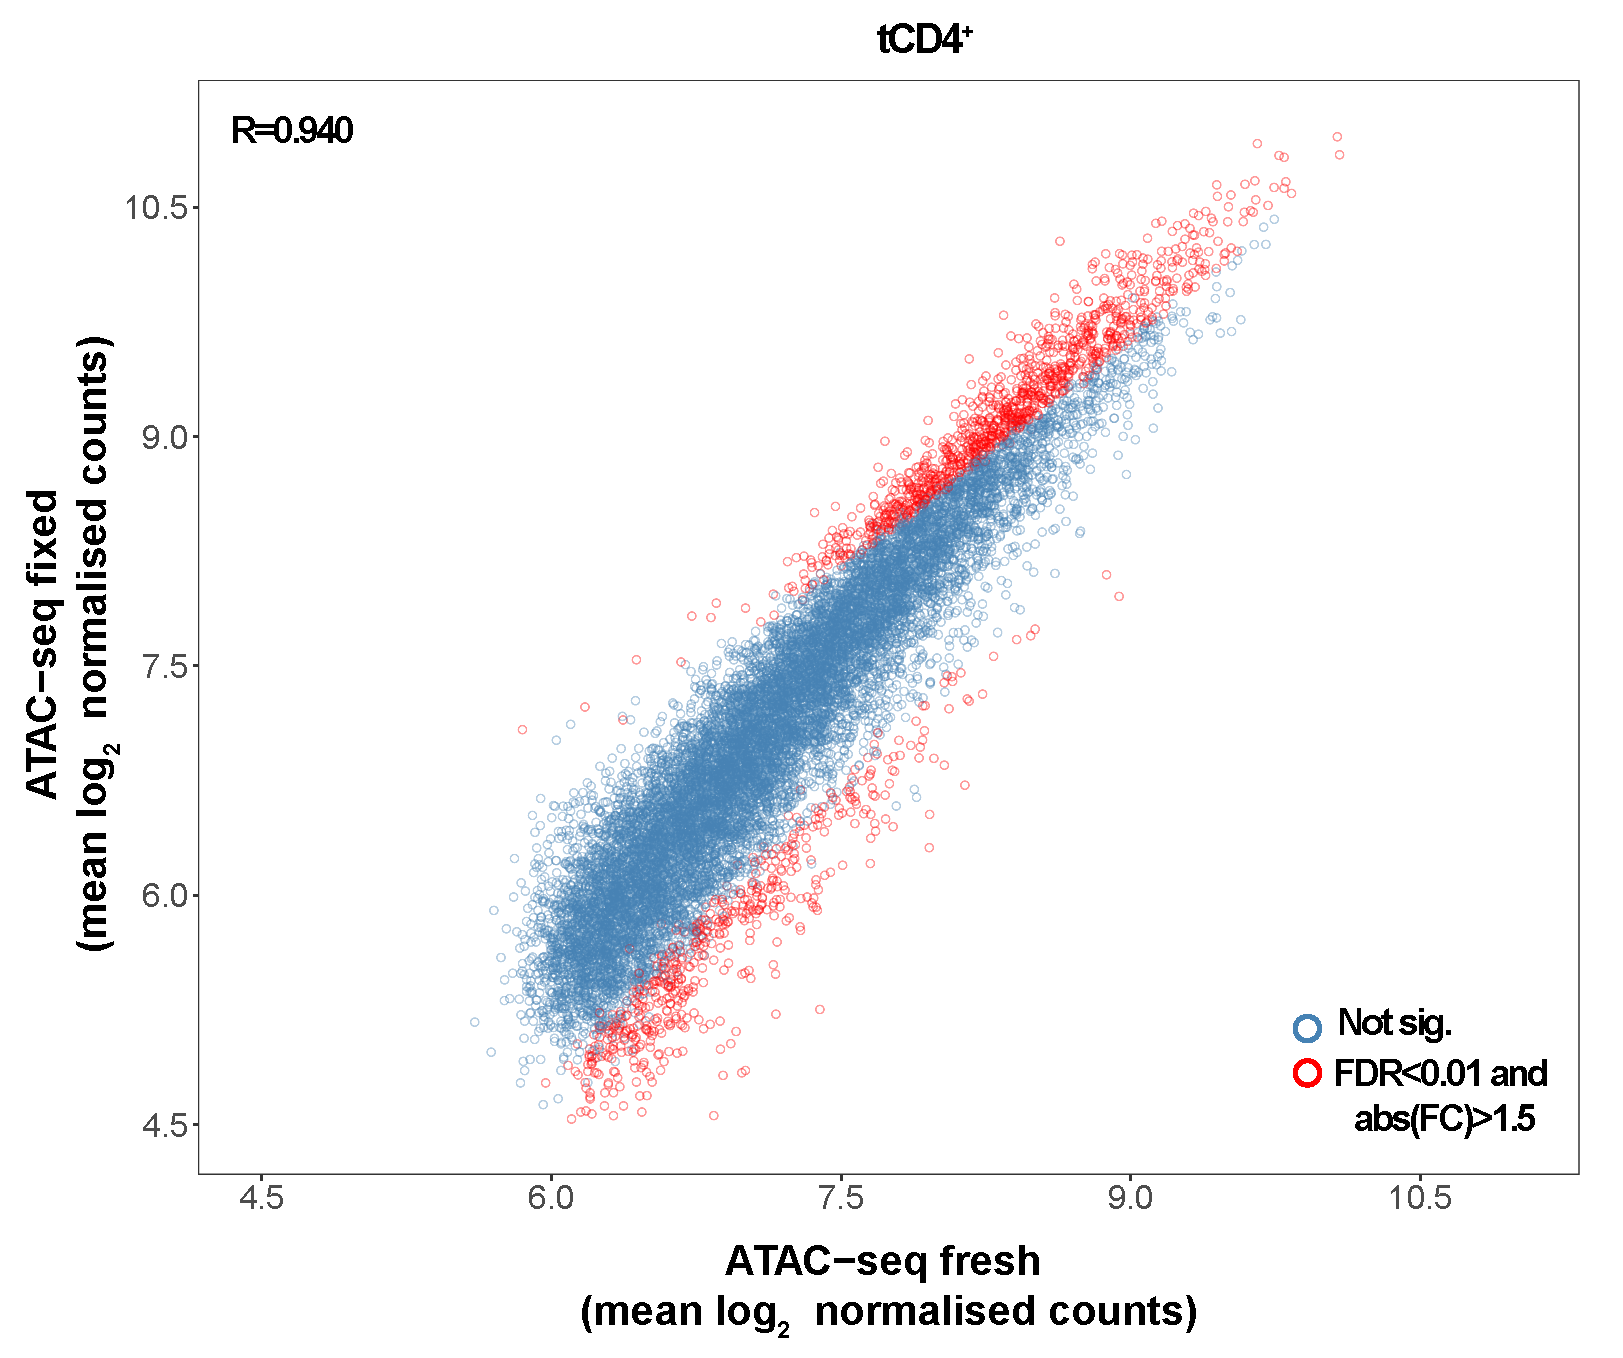
\includegraphics[width=\textwidth]{./Results1/pdfs/Core_ATAC_CD4_fresh_fixed_correlation_counts_small}%
\caption{}
\end{subfigure}
\begin{subfigure}[b]{0.45\textwidth} 
%the [b] prevents offset in subcaptions
\centering
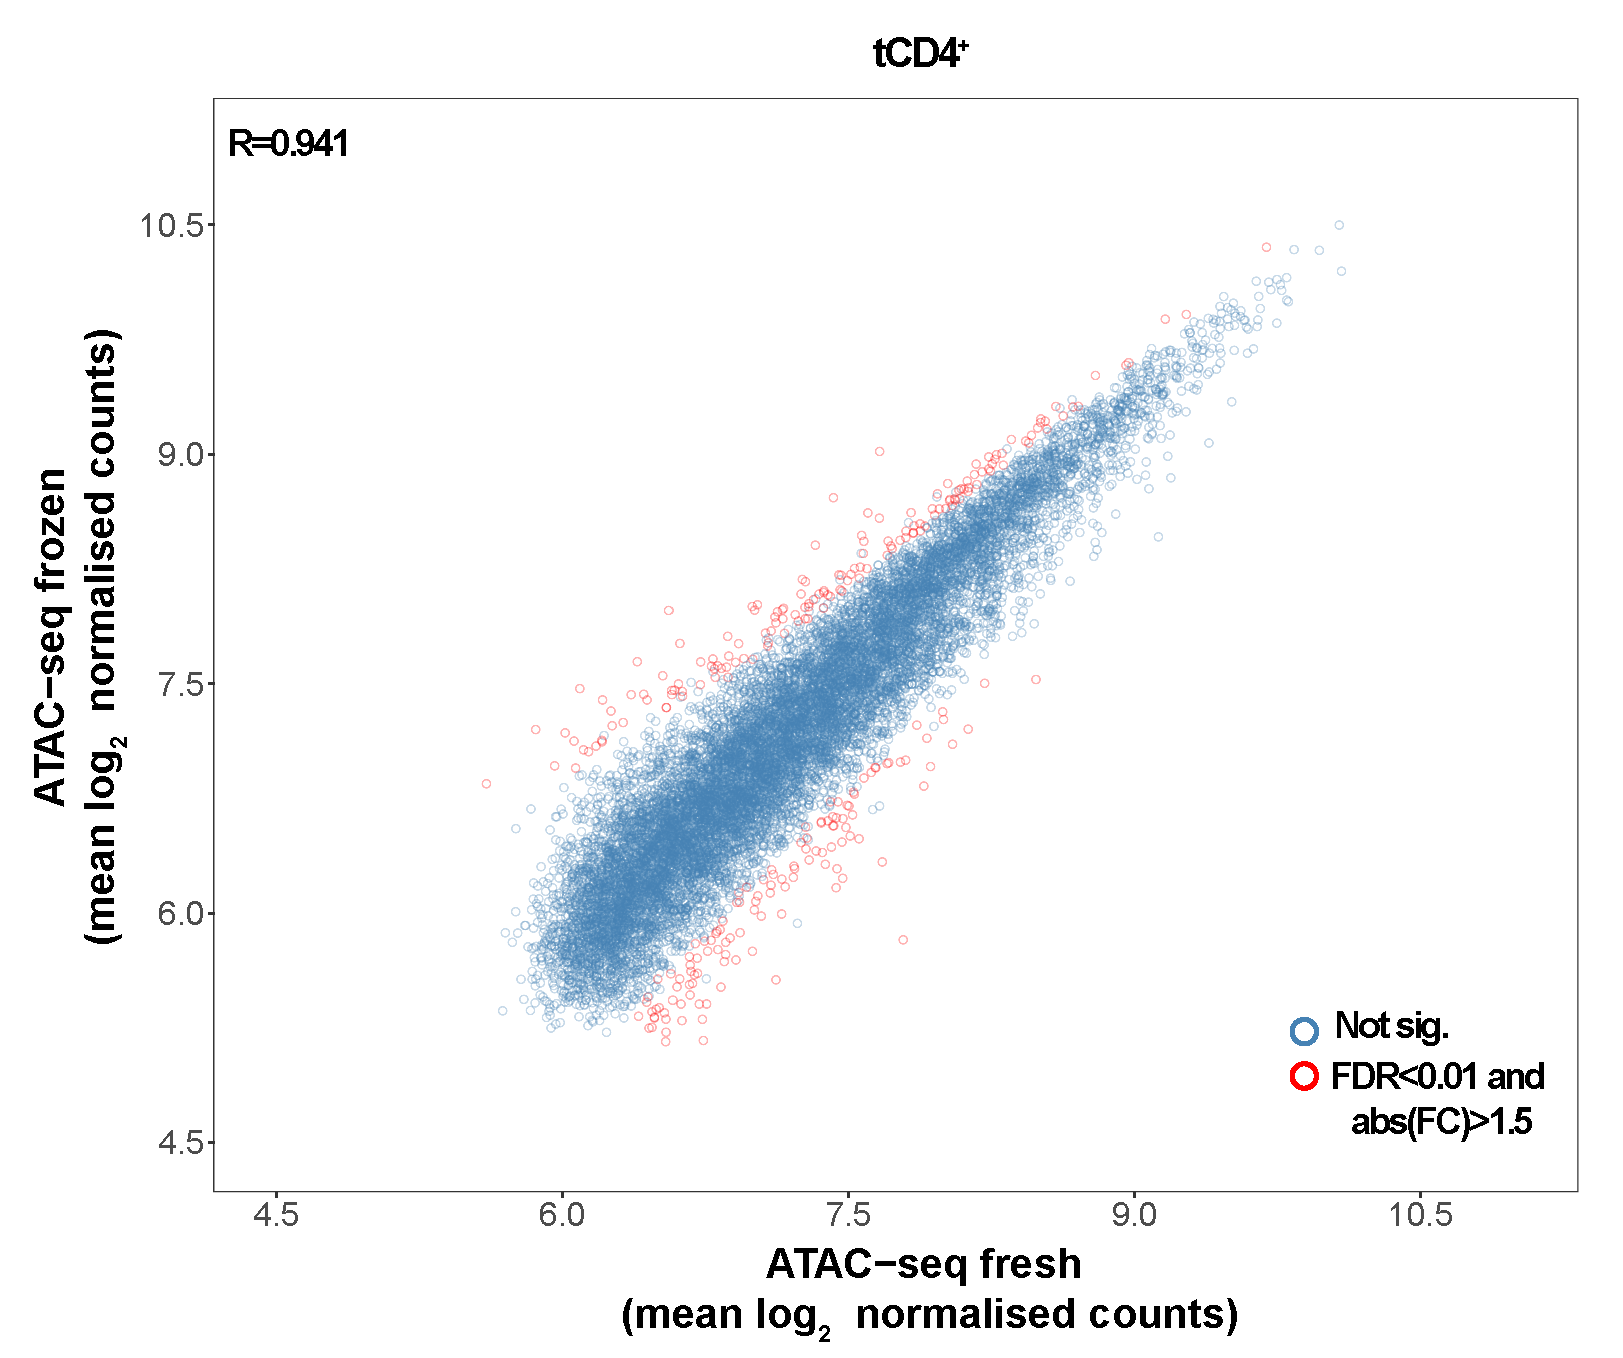
\includegraphics[width=\textwidth]{./Results1/pdfs/Core_ATAC_CD4_fresh_frozen_correlation_counts_small}
\caption{}
\end{subfigure}
\caption[Comparison of the log$_2$ normalised ATAC-seq counts at the consensus master lists peaks in fresh, fixed and frozen conditions.]{\textbf{Comparison of the log$_2$ normalised ATAC-seq counts at the consensus master lists peaks in fresh, fixed and frozen conditions.} Each plot shows the comparison of ATAC-seq log$_2$ mean normalised counts from the ML\_CD14\_all\_cond or ML\_CD4\_all\_cond filtered for background noise (80\% empirical cut-off) between (A) and (C) fresh versus fixed or (B) and (D) fresh versus frozen samples. Pearson correlation coefficient (R) is indicated.}
\label{figure:Core_ATAC_all-conditions_correlation}
\end{figure}
	
	
The regions showing lower correlation in mean counts were significant DARs (FDR$<$0.01 and fold change$>$1.5) when performing differential chromatin accessibility analysis between ATAC-seq fresh and ATAC-seq fixed or frozen at each of the ML\_CD14\_all\_cond and ML\_CD14\_all\_cond regions using DESeq2. The number of significant DARs (FDR$<$0.01 and fold change>1.5) reported in each of the comparisons mirrored the PCA analysis results (Table \ref{tab:Core_ATAC_all_conditions_DARs}). In CD14$^+$ monocytes, the largest number of DARs versus fresh were reported for the ATAC-seq frozen (5,269 regions in Figure \ref{figure:Core_ATAC_all-conditions_correlation}B). Conversely, in CD4$^+$ the greatest differences in chromatin accessibility were found between fresh and fixed ATAC-seq samples (1,564 DARs in Figure \ref{figure:Core_ATAC_all-conditions_correlation}D). In the performance of the differential analysis, the limited samples size (only two ATAC-seq fixed libraries) and the borderline quality of the ATAc-seq CD4$^+$ samples partially skewed the normalisation process, as can be observed by the location of the significant DARs in Figure \ref{figure:Core_ATAC_all-conditions_correlation} d. Altogether, the number of DARs identified in each comparison did not involve more than 14.2\% of the total ATAC-seq regions included in the analysis, representing a discrete proportion of the genome-wide accessible regions studied in this two cell types.  


%To further assess the differences in chromatin accessibility, differential chromatin accessibility analysis between ATAC-seq fresh and ATAC-seq fixed or frozen at each of the ML\_CD14\_all\_cond and ML\_CD14\_all\_cond peaks was performed using DESeq2. The number of significant DARs (FDR$<$0.01) reported for in each of the comparisons mirrored the PCA analysis results (Table \ref{tab:Core_ATAC_all_conditions_DARs}). In CD14$^+$ monocytes, the largest number of DARs (5,269) was reported when comparing ATAC-seq frozen to the fresh reference state. Conversely, in CD4$^+$ the greatest differences in chromatin accessibility were found between fresh and fixed ATAC-seq samples (1,564 DARs).  	
	
	
\begin{table}[htbp]
%\setlength{\tabcolsep}{20pt} only to stretch the columns if you want
%\renewcommand{\arraystretch}{1.5}
\centering
\begin{tabular}{@{} c c c}
\toprule
\textbf{Cell type} & \textbf{Fresh vs Frozen} & \textbf{Fresh vs Fixed} \\
\midrule
\midrule
CD14$^+$ monocytes & 5,269 (12.9\%) & 1,838 (4.5\%) \\
CD4$^+$           & 282  (2.1\%)   & 1,564 (14.2\%) \\
\bottomrule
\end{tabular}
\medskip %gap
\caption[Summary results from the differential chromatin accessibility analysis comparing ATAC-seq frozen or fixed chromatin landscape to the reference ATAC-seq fresh.]{\textbf{Summary results from the differential chromatin accessibility analysis comparing ATAC-seq frozen or fixed chromatin landscape to the reference ATAC-seq fresh.} Number of significant DARs (FDR$<$0.01 and fold change$>$1.5) identified using ML\_CD14\_all\_cond and ML\_CD14\_all\_cond filtered for background counts using 80\% cut-off (optimal cut-off identified for this analysis, data not shown). In brackets are shown the percentage of DARs over the total number of regions included in the differential analysis.}
\label{tab:Core_ATAC_all_conditions_DARs}
\end{table}
\bigskip %bigger space
	
An example of differences in chromatin accessibility between fresh and frozen ATAC-seq libraries in CD14$^+$ included four regions within and downstream of the \textit{TNFSF14} gene (Figure \ref{figure:Core_CD14_differential_TNFSF14}. TNFSF14 is the ligand for a receptor from the TNF-receptor superfamily. TNFSF14 is involved in T cell activation, induction of apoptosis and  also in bone destruction mediated by monocytes and synovial cells interactions in RA. Three of the DARs were located at the promoter, an exon and the 3'UTR of the gene (respectively) and one was found at approximately 5Kb upstream the gene. All DARs were more open in ATAC-seq frozen libraries when compared to fresh and did not show any changes between fresh and fixed conditions.%\parencite{} 
%The interaction of monocytes with rheumatoid synovial cells is a key step in LIGHT-mediated inflammatory bone destruction.

	
	
	
\begin{figure}[htbp]
\centering
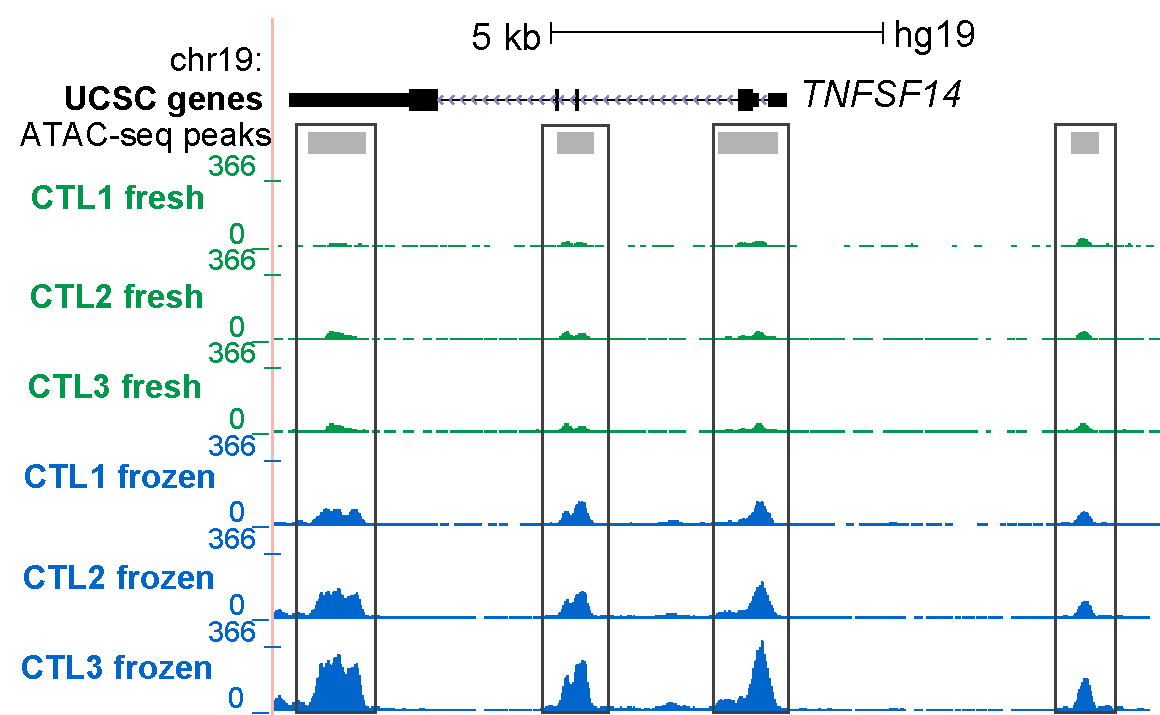
\includegraphics[width=0.65\textwidth]{./Results1/pdfs/Core_CD14_TNFSF14_track_UCSC}
\caption[Differential chromatin accessibility at the \textit{TNFSF14} gene between ATAC-seq fresh and ATAC-seq frozen in CD14$^+$ monocytes.]{\textbf{Differential chromatin accessibility at the \textit{TNFSF14} gene between ATAC-seq fresh and ATAC-seq frozen in CD14$^+$ monocytes.} UCSC Genome Browser view illustrating the normalised read density (y-axis) at four significant (FDR$<$0.01 and fold change$>$1.5) DARs (x-axis) within and upstream the \textit{TNFSF14} gene in CD14$^+$ monocytes. The four DARs were more accessible in ATAC-seq frozen when compared to ATAC-seq fresh. ATAC-seq fixed was similar to ATAC-seq fresh at these four locations. Tracks are colour-coded by condition(green=fresh, blue=frozen and red=fixed).}
\label{figure:Core_CD14_differential_TNFSF14}
\end{figure} 	



\section{Discussion}

The aim of this chapter was to establish a data analysis pipeline for ATAC and compare various experimental protocols, as this was the first time this technique was used in the research group. A particular focus was to consider appropriate methodologies for clinical studies, where sample availability and quality may be severely limiting, and a number of alternative protocols, metrics and algorithms described in early ATAC reports were evaluated in the pilot experiment presented in this chapter. This enabled the establishment of a pipeline and approach to be implemented for investigation of psoriasis and PsA chromatin landscape (Chapters \ref{ch:Results2} and \ref{ch:Results3}).

\subsection{ATAC: methodological aspects and pipeline establishment}

At the time of the first ATAC-seq publication \parencite{Buenrostro2013}, well established protocols for complete processing and data analysis of ATAC were lacking. Since then, several publications have implemented ATAC-seq and modifications of this protocol together with a wide range of data analysis strategies to answer different biological questions (Table \ref{tab:ATAC_comparative_methods}) as well as alternative protocols such as THS-seq to assess chromatin accessibility in low number of cells.

The data and analysis presented in this chapter has confirmed some limitations of the ATAC-seq and Fast-ATAC protocols. Quality assessment and variability across samples was difficult to detect through pre-sequencing library quality control based on relative abundance of the different DNA fragment sizes. Successful profiles of DNA relative abundance for the ATAC libraries, showing nucleosome patterns would still lead to libraries with high background noise when visualising read density in the UCSC Genome Browser. This required the identification and establishment of appropriate data analysis and quality control measures beyond pre-sequencing library quality assessment.

In this chapter different quality metrics were explored, including TSS enrichment and FRiP. Both correlated well with the overall differences in sample quality from the ATAC-seq libraries used as an exemplar here. Importantly, TSS and FRiP were shown to be independent of sequencing depth, and therefore can be applied in low depth sequenced samples when performing optimisation or preliminary quality control before increasing the coverage, as also recently shown in other studies \parencite{Corces2017}. Similarly to TSS, FRiP proved to be informative in evaluating signal-to-noise ratios; however it relies on peak calling and thus is more likely to be biased. In agreement with these findings, enrichment of ATAC signal across Ensembl annotated TSS is now recommended by ENCODE as the preferred means of assessing overall sample quality, and was implemented as the metric to evaluate signal-to-noise in our pipeline. 

The variability in quality of the ATAC-seq and Fast-ATAC libraries was also addressed at the peak calling level in this chapter, with the implementation of a peak filtering strategy that for each particular sample could identify good quality and reproducible peaks using IDR analysis between pseudoreplicates. This approach was demonstrated to reduce  repetitive and non meaningful regions that could be confounder for downstream analysis. In terms of sequencing depth, analysis in this chapter showed 20 to 25 million reads after filtering to be the required minimum sufficient to identify an appropriate proportion of accessible regions (peaks) as well as to obtain meaningful results in the peak filtering based on pseudoreplicate IDR analysis. These observations have also been confirmed by Qu and colleagues \parencite{Qu2017}, where IDR analysis used to evaluate consistency across replicates but not implemented for peak filtering.

Establishment of appropriate measurements for post-sequencing library quality control allowed formal testing of the effect of transposition times, one of the most critical variables in ATAC that can be cell type specific, beyond the conditions from Buenrostro's publication. At the start of the project transposition for 40 min appeared the most appropriate for all cell types according to pre-sequencing library quality control (relative abundance of DNA library fragment sizes). Assessment of three different transposition times in the ATAC-seq protocol showed heterogenous impact across cell types on the ratio of NFF/NBF and overall no major impact on signal-to noise ratios. The use of the improved Fast-ATAC protocol addressed some of the limitations identified by the ATAC-seq data generated within our group. Specifically, Fast-ATAC significantly reduced the percentage mitochondrial reads in all four cell types of interest for this thesis. In contrast, the improvement of signal-to-noise for hematopoietic cells claimed by the Fast-ATAC paper was not evident. In fact, Corces and colleagues only showed improved TSS by Fast-ATAC in CD4$^+$ T cells \parencite{Corces2016}. The publication of Omni-ATAC and a comprehensive comparison of the three ATAC protocols across a large number of cell types demonstrated that Fast-ATAC did not improve TSS fold-enrichment when compared to ATAC-seq in some of the hematopoietic cells, for example CD19$^+$ cells, consistent with the finding in the systematic comparison using pilot data in this thesis.

pre-sequencing library quality control based on relative abundance of the different DNA fragment sizes. Successful profiles of DNA relative abundance for the ATAC libraries,



\subsection{The challenges of performing differential chromatin accessibility analysis}
%Until ATAC-seq release, limited research had been performed to investigate differences in chromatin accessibility, and mainly used data from cell lines \parencite{Degner2012}. 
Studying chromatin accessibility in clinical samples first requires the definition of a consensus master list of accessible regions for which no accepted method has been agreed. In this work, a master list containing all the peaks identified in at least 30\% of the samples included in analysis has been chosen. This represents an unbiased approach to include peaks that can vary across individuals (regardless of biological subgroup) but still be differentially accessible across conditions. Other publications have preferred building condition-specific master lists or simply include all the significant peaks called in all the analysed samples \parencite{Alasoo2018, Thurner2018}. 

When used for differential analysis, an additional filtering step to account for high read counts in peaks that were absent in some of the samples (background counts) has been implemented. In terms of the algorithm to perform normalisation and differential chromatin accessibility analysis, no consensus has been reached in the literature. The majority of the studies reviewed at the time of implementing differential analysis were peak-based and relied on RNA-seq or microarray algorithms such as EdgeR, limma or DESEq2 (Table \ref{tab:ATAC_comparative_methods}). The analysis here performed, revealed DESeq2 as a more stringent method compared to quantile normalisation\&limma voom. Limma has been reported to be affected by low quality samples and that may also explain the increase in differential hits observed when compared to DESEq2 \parencite{Alasoo2018}. For both methods, the implementation of the additional filtering cut-off to control for high number of background reads has shown a reduction in the number of significant differentially accessible regions. Given the difficulties of obtaining large number of high quality samples in a clinical setting, DEseq2 in combination with the additional filtering step to control to some extent for potential false positive appeared was chosen as an appropriately stringent method at the time study. As specific tools for ATAC analysis are developed, further comparison of the outputs will be of interest in future work.


\subsection{Studying the chromatin landscape from psoriasis biopsies}
At the time of writing, only RNA-seq studies have been performed in keratinocytes from psoriasis skin biopsies. The relevance of keratinocytes in psoriasis pathophysiology and the ability to sample the tissue represented a great opportunity to investigate the chromatin accessibility landscape at the main site of inflammation using ATAC. Variations of the ATAC-seq protocol (with different NP40 and Tn5 conditions) ATAC 1, ATAC 2 and Fast-ATAC were found to perform very poorly in keratinocytes isolated from skin biopsies and also in cultured NHEKs. The fact that similar results were obtained in keratinocytes isolated through different systems as well as in NHEKS indicated that the main reason for poor performance of these protocols was intrinsic to the cell type and not driven by compromising cell viability through the system used to isolate the cells. As differentiation progresses, keratinocytes synthesis an insoluble protein structure that progressively replaces the plasma membrane, which may have been impairing appropriate cell permeabilisation and efficient transposition. Interestingly, using increased Tn5 concentration to perform appropriately in NHEKS did not appear to improve ATAC quality libraries in the data presented. Similarly, the additional optimisation of the Fast-ATAC protocol modifying the concentration of detergent and Tn5 also failed to improve the quality of the data.

Recent release of the Omni-ATAC protocol and testing here showed substantially improved performance vs ATAC-seq and Fast-ATAC in keratinocytes. The data was consistent with Corces \textit{et al.}, 2017, where consistent successful results in NHEKs were shown, and it encourages future testing of Omni-ATAC in keratinocytes from psoriasis patients biopsies processed through adherent assay to minimise the presence of dead cells. This opens a new avenue to explore the chromatin landscape in lesional and uninvolved psoriasis biopsies.


\subsection{Characterisation of the effect of preservative techniques in the chromatin landscape}
The use of clinical samples sometimes involves logistical limitations that require sample preservation. At the time of starting this thesis the Oxford Genomics Centre at the WHG had implemented the use of DSP as a compatible fixative for microfluidics-based scRNA-seq methods. It was therefore of interest to test the ability of this fixative to perform well in ATAC \parencite{Attar2018}. Alternatively cryopreservation of PBMCs had historically been used but formal assessment of the effect of this process in the chromatin landscape of different cell types had not yet been conducted.

DSP fixed samples presented overall lower abundance of NFF, when compared to the fresh and frozen libraries. DSP performed very poorly in the two cell types from CTL1, which presented extremely low abundance of NFF and predominance of NBF. Interestingly, despite the abundance of di-nucleosome fragments in these two samples, the chromatin structure across the TSS failed to reproduce the position of the TSS flanking nucleosome, which could be due to nucleosome displacement, as DSP does not cross-link DNA to proteins. Since this effect was only observed for CTL1, problems relating to inappropriate performance of the fixation protocol on that particular day may be the cause.

After removing the CTL1 samples, consideration of the chromatin accessibility landscape in all the remaining samples clearly showed that the differences by condition were greater than the differences between individuals. This was confirmed by performing differential analysis, which revealed a moderate number of DARs when comparing fixed or frozen to the fresh reference ATAC-seq. As expected, CD14$^+$monocytes appeared to be more sensitive to cryopreservation than CD4$^+$ cells and present greater differences in the chromatin accessibility landscape when compared to fresh samples. This has been previously reported in the context of cytokine response, where cryopreservation of monocytes and immunature DCs have shown a skewed profile compared to fresh counterparts \parencite{Meijerink2011}. 

The results presented here could be limited by the borderline quality of some of the libraries, as previously explained, which was due to the issues of consistency intrinsic to the ATAC-seq protocol and could be distorting the findings to some extent. Nevertheless, this study still provides some useful information regarding the effect of using DSP in sorted cell populations or cryopreserved PBMCs. Depending on the sample size foreseen in each particular study, if the aim is to perform paired ATAC and scRNA-seq based on microfluidics methods in the same samples, and the final biological question, these two preservative protocols could be considered for implementation. Additionally, as the ATAC-seq protocol has been improved, ATAC has also been successfully conducted in frozen tissues and formaldehyde samples and can be considered when establishing the experimental design \parencite{Corces2017, Chen2016}. In this thesis, since the sample size was limited and the main question was to assess the chromatin landscape as close as possible to \textit{in vivo} disease conditions, fresh cells were used to generate the results presented in the following two chapters.

\subsection{Conclusions}
The work described here has compared commonly used strategies from ATAC publications in order to establish an appropriate method to perform chromatin accessibility analysis in the context of psoriasis and PsA, maximising the use of samples in a clinical setting whilst accounting for some quality limitations and the resources and expertise in the group available at the time. A robust pipeline was established and conclusions drawn regarding optimized protocols and conditions. As ATAC has become a more commonly used technique, new methods and updates have been introduced on both in the experimental protocol and analysis side which means that data presented throughout this thesis could be revisited in the future with further optimised analytical methods. Moreover, the implementation of Omni-ATAC for future sample recruitment is likely to further improve the quality and confidence in reported differentially open regions.
